\documentclass[12pt,a4paper]{report}

\usepackage[utf8]{inputenc}
\usepackage{colortbl}
\usepackage{url}
\usepackage{fancyhdr}
\usepackage[margin=1in]{geometry}
\usepackage{lipsum}
\usepackage{times}
\usepackage{graphicx}
\usepackage{multirow}
\graphicspath{ {images/} }
\usepackage{wrapfig}
\usepackage{rotating}
\usepackage[singlelinecheck=false,justification=Centering]{caption}
\usepackage{acro}
\usepackage{subfig}
% probably a good idea for the nomenclature entries:
\acsetup{first-style=short}

% class `abbrev': abbreviations:
\DeclareAcronym{sql}{
	short = SQL ,
	long  = Standardized Query Language ,
	class = abbrev
}
\DeclareAcronym{orm}{
	short = ORM ,
	long  = Object Relational Mapper ,
	class = abbrev
}
\DeclareAcronym{ai}{
	short = AI ,
	long  = Artificial Intelligence ,
	class = abbrev
}
\DeclareAcronym{cli}{
	short = CLI ,
	long  = Command Line Interpreter ,
	class = abbrev
}
\DeclareAcronym{mvc}{
	short = MVC ,
	long  = Model View Controller ,
	class = abbrev
}
\DeclareAcronym{mvp}{
	short = MVP ,
	long  = Model View Presenter ,
	class = abbrev
}
\DeclareAcronym{mvvm}{
	short = MVVM ,
	long  = Model View View Model ,
	class = abbrev
}
\DeclareAcronym{ux}{
	short = UX ,
	long  = User Experience ,
	class = abbrev
}
\DeclareAcronym{ui}{
	short = UI ,
	long  = User Interface ,
	class = abbrev
}
\DeclareAcronym{sdk}{
	short = SDK ,
	long  = Server side rendering ,
	class = abbrev
}
\DeclareAcronym{vsc}{
	short = VSC ,
	long  = Visual Studio Code ,
	class = abbrev
}
\DeclareAcronym{rest}{
	short = REST ,
	long  = Software Development Kit,
	class = abbrev
}
\DeclareAcronym{ssr}{
	short = SSR ,
	long  = Server side rendering ,
	class = abbrev
}
\DeclareAcronym{pwa}{
	short = PWA ,
	long  = Progressive web app ,
	class = abbrev
}
\DeclareAcronym{3d}{
	short = 3D ,
	long  =Three Dimensional ,
	class = abbrev
}
\DeclareAcronym{php}{
	short = PHP ,
	long  = Hypertext Preprocessor  ,
	class = abbrev
}
\DeclareAcronym{os}{
	short = OS ,
	long  = Operating System  ,
	class = abbrev
}

\DeclareAcronym{ide}{
	short = IDE ,
	long  = Integrated Development Environment  ,
	class = abbrev
}
\DeclareAcronym{us}{
	short = U.S ,
	long  = User Story  ,
	class = abbrev
}

\DeclareAcronym{uml}{
	short = UML ,
	long  = Unified Modeling Language  ,
	class = abbrev
}
\DeclareAcronym{api}{
	short = API ,
	long  = Application Program Interface  ,
	class = abbrev
}
\DeclareAcronym{rtl}{
	short = RTL ,
	long  = Register Transfer Level  ,
	class = abbrev
}
\DeclareAcronym{gui}{
	short = GUI ,
	long  = Graphical User Interface ,
	class = abbrev
}
\DeclareAcronym{html}{
	short = HTML ,
	long  = Hypertext Markup Language  ,
	class = abbrev
}
\DeclareAcronym{ucd}{
	short = UCD ,
	long  = Use Case Diagram  ,
	class = abbrev
}

\linespread{1.5}
\setlength{\parindent}{6ex}
\usepackage{float}
\usepackage{indentfirst}
\usepackage{color, colortbl}
\usepackage{caption} 
\setcounter{secnumdepth}{3}
\setcounter{tocdepth}{3}
\usepackage{pdfpages}
\renewcommand{\contentsname}{\centering Table of Contents}
\definecolor{LightCyan}{rgb}{0.88,1,1}
\usepackage{titletoc}
%\titlecontents{section}[left]{above-code}{numbered-entry-format}{numberless-entry-format}{filler-page-format}[below-code]
\newcommand{\setupname}[1][\chaptername]{
	\titlecontents{chapter}[0pt]{\vspace{1ex}}{\bfseries#1~\thecontentslabel:\quad}{\bfseries}{\bfseries\hfill\contentspage}[]
}
\begin{document}
	
	
\includepdf[pagecommand={\thispagestyle{empty}},pages=-]{Page-de-garde.pdf}
	
	
	\pagenumbering{roman}   %set page numbering to roman%	
	\setcounter{page}{1}
	
	\chapter*{\centering Acknowledgment}
	\addcontentsline{toc}{chapter}{Acknowledgement}
	
	I would like to express my deepest appreciation to all those who aide me to complete this report.  A special gratitude is giving to my final year project  manager, Mr. \textsc{Bayrem TRIKI}, whose contribution in stimulating suggestions and encouragement,  helped me to coordinate this project especially in writing this report.\\
	
	 A special thanks goes to my supervisor Mr. \textsc{Anis Ben Bettaieb}, who guided me throughout the development of  \textbf{``Cake it up !''} application.\\
	
	Furthermore I would also like to acknowledge with much appreciation the crucial role of \textbf{Anypli} company, who gave the permission to use all required  equipment and the necessary materials to complete this project. \\
	

	Finally, I have to appreciate the guidance will be given by other supervisor, especially in my project exposition that will surely improve my presentation skills thanks to their comment and advices.
	\cleardoublepage
	\chapter*{\centering Dedication}
	This report is dedicated to my mother \textbf{Fatiha}, for her kindness and devotion, and for her endless support, thanks for always being there for me.
	I would like to express my gratitude towards my father  \textbf{Mohamed} who is my role model and mentor.\\
	
	 My sisters \textbf{Khawla}, \textbf{Imen}, \textbf{Ikhtiyar} and \textbf{Wafa} who were more than helpful morally, so proud to have them as my backup.\\
	 
	  A special thanks goes to the one who is the most helpful and supporting person I know \textbf{Ahmed}, thank you so much for being there for me.\\
	  
	  Finally I would like to thank my best friends \textbf{Sirine}, \textbf{Ons} and \textbf{Sarra} for standing by me at all costs, which made it easy for me to get past all the difficult situation. \\
	%content
	\cleardoublepage
	\tableofcontents
	\cleardoublepage
	\addcontentsline{toc}{chapter}{\listfigurename} 
	\listoffigures	
	\cleardoublepage
	\addcontentsline{toc}{chapter}{\listtablename} 
	\listoftables	
	\clearpage 
	\addcontentsline{toc}{chapter}{List of Abbreviations}
	\printacronyms[include-classes=abbrev,name=List of Abbreviations]
	\cleardoublepage
	\pagenumbering{arabic} 
	\setcounter{page}{1}
	
	
	\chapter*{\centering General introduction}
	\addcontentsline{toc}{chapter}{General introduction}
	Bakeries are a popular type of food-service establishment, and they allow you to express your culinary creativity while also serving a unique market, the problem is you can spend all day and night in the kitchen creating the next best cake, but if no one knows about it, all that hard work will go in vain.  \par 
	Evidently bakeries are facing difficulties attracting customers and handling their orders and products, in fact even clients find it difficult to find a pastry to their taste without having to go through the process of searching and asking around for opinions.\par
	In order to succeed in the bakery business,  some marketing and advertising can also make a big difference.\par
	
	Depending on all of that, we are providing as a solution an application named \textbf{``Cake it up !''} that fills in the needs of both parts the business owner and the client. It provides an easy way for the owner to promote their business and easier way for the client to find a place that matches him.\par
	This report contains six chapters;\par
	The first chapter is a quick presentation of the company \textbf{``Anypli''} where the internship took place, this chapter will also contain the preliminary Study of the project, in fact we will be analyzing the existing and explaining our solution.  \par
	The second chapter focuses on the requirements of the project and the planning of this work, where we will present the breakdown of this project needed to highlight the different modules to be developed in time.\par
	The third chapter will provide the means used to make this work possible and give a detailed description of the project's architecture.
	\par
	In the fourth, fifth and sixth chapter, we will present the three releases of this work. This step is based on the AGILE SCRUM methodology for the purpose of good project management.\par
	
	We conclude with a general conclusion that presents an analysis of the work done within \textbf{``Anypli''} company. This section highlights not only a summary of the work done throughout the period of the end-of-course project internship but also proposals from the various perspectives.\par
	
	\pagestyle{fancy}
	\fancyhf{}
	\fancyhead[LE,RO]{\leftmark}
	\fancyfoot[CE,CO]{\thepage}
	\renewcommand{\footrulewidth}{0.4pt}
	\setupname
	\chapter{Project scope }
	\section*{Introduction}
	\addcontentsline{toc}{section}{Introduction}
	This chapter will be dedicated to the presentation, in the first place, of the environment in which our project was realized while taking into account the efficiency and the quality of the work.\par
	Secondly, we will present the project itself, analyzing the existing and proposing a solution that will allow us to provide elements of response to the shortcomings identified.\par
	finally, we will give a brief and clear idea about what methodology was used to make this project.
	\section{Host organization Presentation}
	\textbf{``Anypli''} is a web and mobile development agency, founded in 2011 and located at Monastir, it has over 50 employees. it is in possession of several teams of enthusiasts each mastering their area of expertise as well as related fields. \textbf{``Anypli''} follows a methodology based on listening and consulting in order to offer quality achievements perfectly suited to the objectives of its customers and the resources they want to devote to it. \par
	\begin{figure}[H]
		\centering
		
\includegraphics[width=3in,keepaspectratio]{logo_anypli.png}
		\caption{Logo Anypli}
		
	\end{figure}
	\textbf{``Anypli''} offers multiple services such as :
	\begin{itemize}
		\item Mobile applications: IOS, Android
		\item Web sites
		\item Design
		\item \ac{ui} and \ac{ux}
		
	\end{itemize}
	\section{Project Presentation}	
	
	\subsection{Analysis of the existing}
	We are in an era where technology leads everything, there is an application for most of the people's needs, however most of these softwares lack some details that are not yet fulfilled.\par
	This section will start by listing some of the applications or ways people use to get information about pastries, then criticize every one of them to show what is missing.
	
	\subsubsection*{Social media}
	The mostly common way is using the social media such as \textbf{``FACEBOOK''} and \textbf{``INSTAGRAM''} where you can find a verity of choices and number of opinions that can guide the user to select the right place. \cite{articalefacebook}\par We can also use it to figure out the cost of the meal or get direction as shown in Figure \ref{label-facebook}.
	\par The social media also give you the ability to communicate with the manager of the place in private to either pass an order or to ask for more details regarding a specific product.  \par
	\begin{figure}[H]
		\centering
		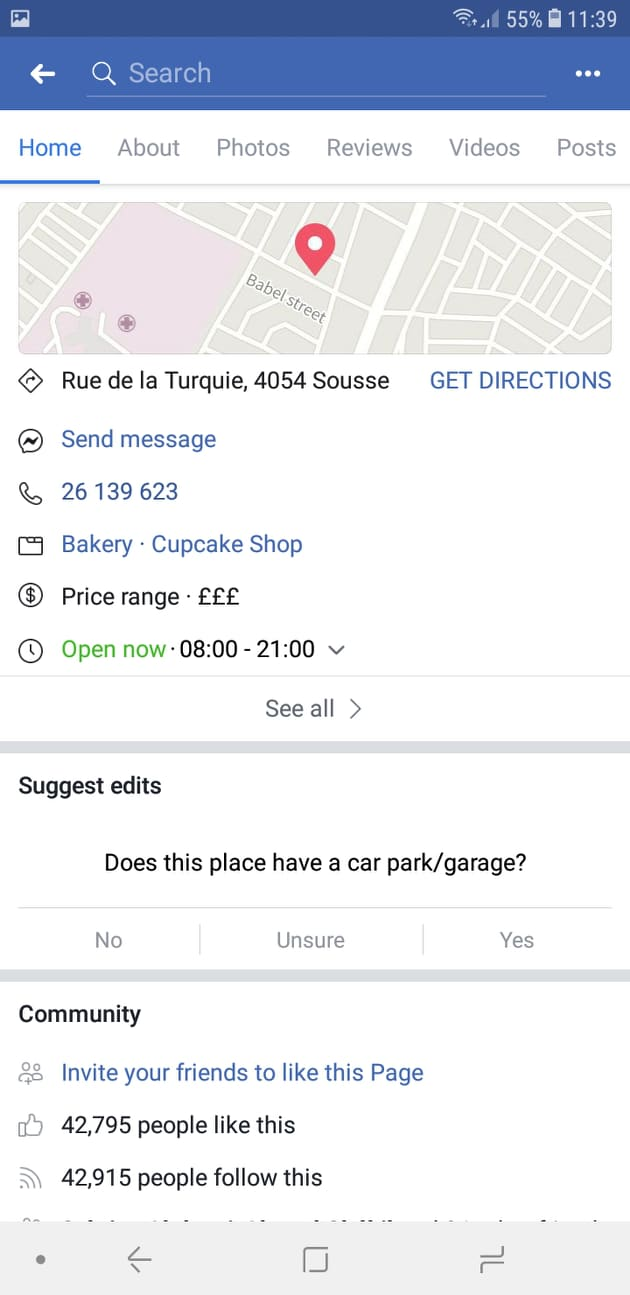
\includegraphics[width=3in,keepaspectratio]{facebook.jpg}
		\caption{Application: FACEBOOK\protect\refstepcounter{footnote}\protect\footnotemark[\thefootnote]}
		
		\label{label-facebook}
	\end{figure}
	\footnotetext[\thefootnote]{Source: https://www.facebook.com/}
	\clearpage
	\subsubsection*{Google maps}
	\textbf{``Google maps''} has been popular for quite a while now, it can be used to figure out the nearby pastries, reviewing shop and get directions as showing in Figure \ref{label-googlemaps}. \par
	\begin{figure}[H]
		\centering
		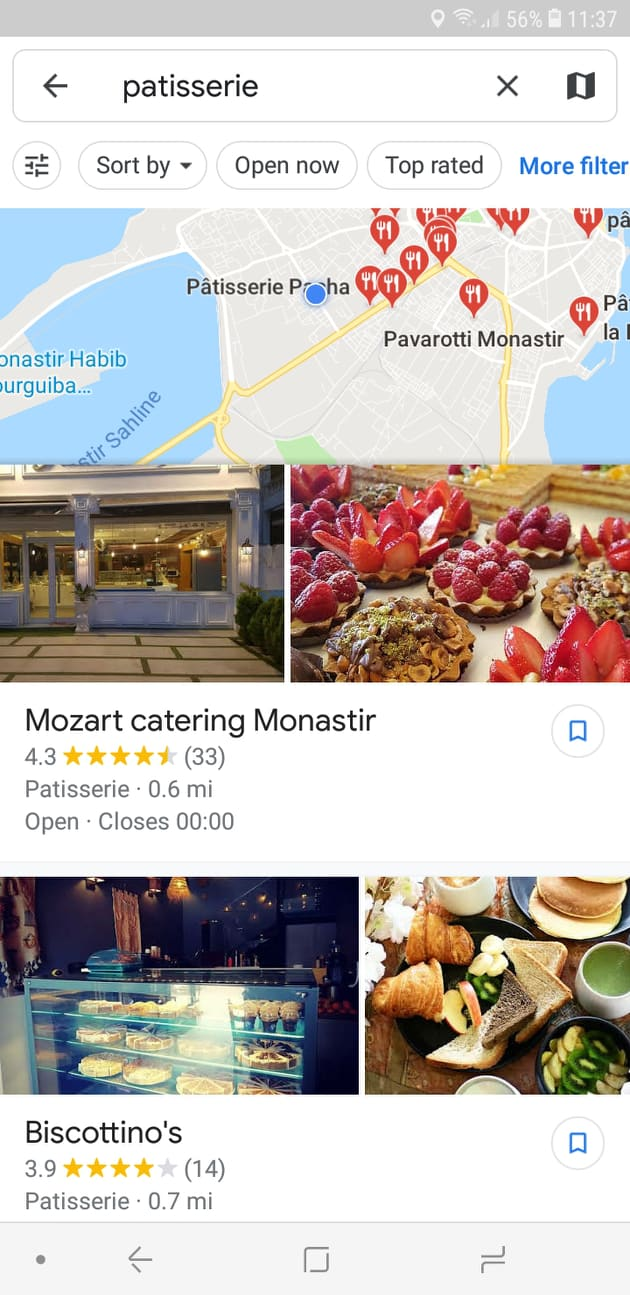
\includegraphics[width=3in,keepaspectratio]{googlemaps.jpg}
		\caption{Google maps\protect\refstepcounter{footnote}\protect\footnotemark[\thefootnote]}
		
		
		
		\label{label-googlemaps}
	\end{figure}
	\footnotetext[\thefootnote]{Source: https://www.google.com/maps}
	\clearpage
	\subsubsection*{Bakery days}
	\textbf{``Bakery days''} gives you the ability to design your cake as presented in Figure  \ref{label-zomato}:
	
	
	\begin{figure}[H]
		\centering
		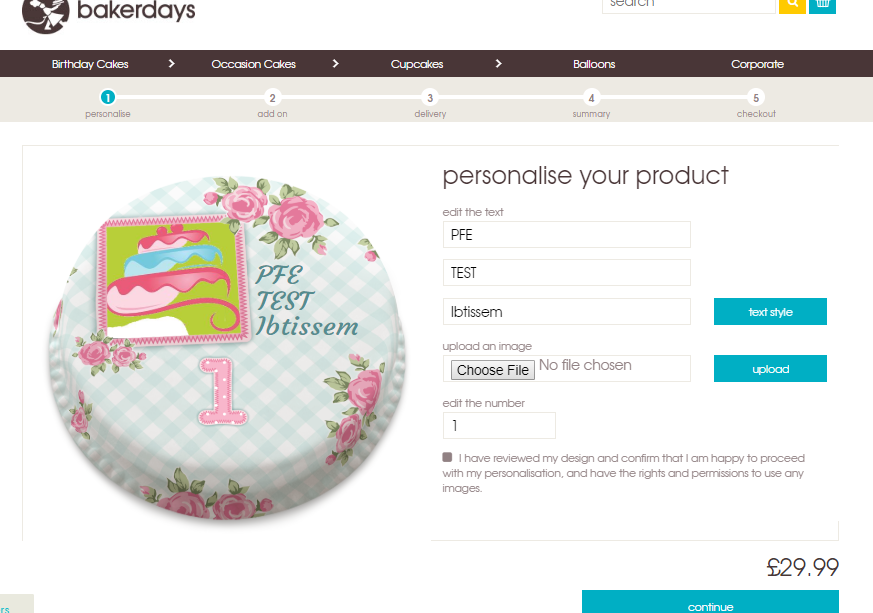
\includegraphics[width=7in,keepaspectratio]{bakerydays.png}
		\caption{Web site: Bakery days\protect\refstepcounter{footnote}\protect\footnotemark[\thefootnote]}
		
		\label{label-zomato}
	\end{figure}
	\footnotetext[\thefootnote]{Source: https://www.bakerdays.com/}
	\subsubsection*{YELP}
	\textbf{``Yelp''} has tremendous power in the pastries industry, and having a strong backing of positive Yelp reviews is like having a flock of golden geese reviews from Yelp can do wonders for any business.\par 
	Advantages of \textbf{``Yelp''}:
	\begin{itemize}
		\item The application provide two parts, the business owner's section presented in Figure \ref{label-yelp1} and the visitor in Figure \ref{label-yelp2}.
		\item  The user can add his own business by adding as many details as possible.
		\item He can respond to the reviews.
		\item Manage his shop.
		\item A visitor can rate and review a shop.
		
	\end{itemize}
	\begin{figure}[H]
		\centering
		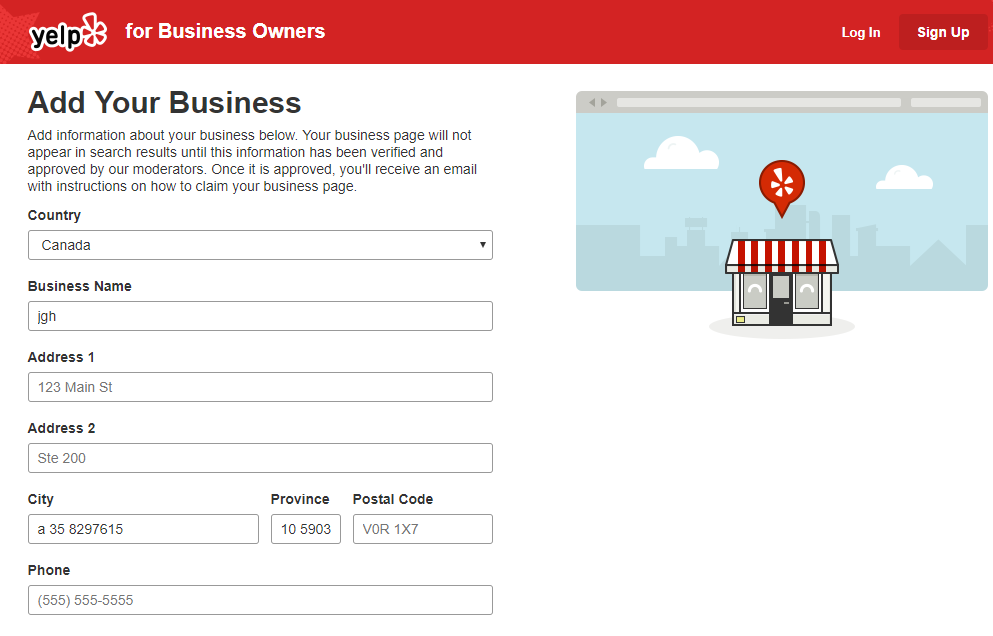
\includegraphics[width=5in,keepaspectratio]{yelp.png}
		\caption{Web application: Yelp (business owner)\protect\refstepcounter{footnote}\protect\footnotemark[\thefootnote]}
		
		
		\label{label-yelp1}
	\end{figure}
	\footnotetext[\thefootnote]{Source: https://biz.yelp.ca}
	\begin{figure}[H]
		\centering
		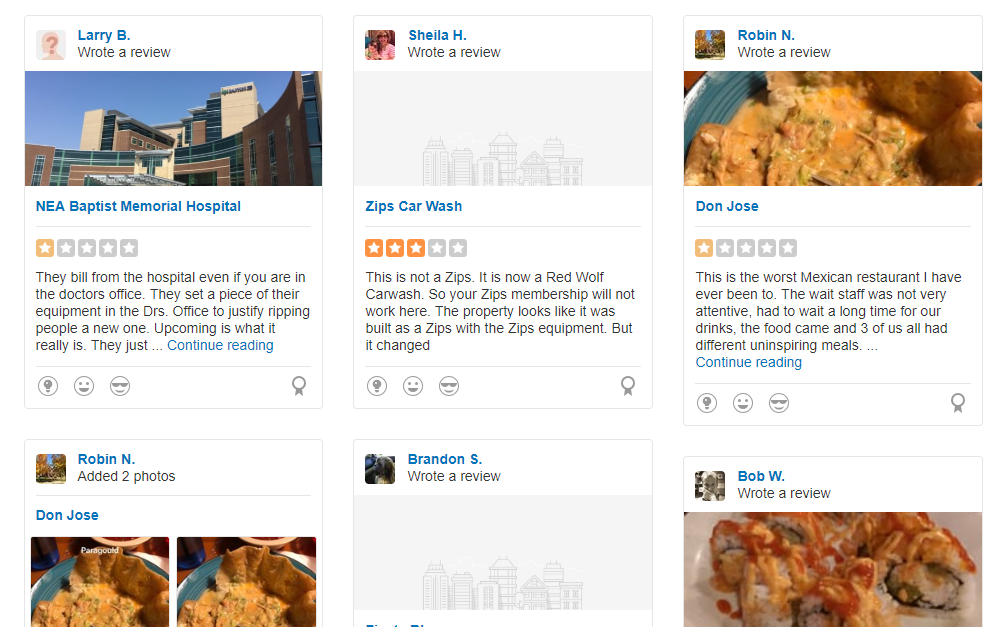
\includegraphics[width=5in,keepaspectratio]{yelp2.png}
		\caption{ Web application: Yelp (user)\protect\refstepcounter{footnote}\protect\footnotemark[\thefootnote]}
		
		
		\label{label-yelp2}
	\end{figure}
	\footnotetext[\thefootnote]{Source: https://www.yelp.com}
	\subsection{Criticism of the existing}
	As shown in Table \ref{table-criticism}, there are number of disadvantages that can not be ignored.
	\begin{table}[H]
		\begin{center}
			\captionsetup[table]{skip=10pt}
			\caption{\label{table-criticism} List of disadvantages of the existing.}
			\setlength\doublerulesep{0.5pt}
			\begin{tabular}{| l | p{13cm} |}
				\hline 
				\rowcolor{LightCyan}
				\textbf{ Existing} & \textbf{Disadvantages} \\ \hline\hline\hline
				Social media       &                        
				\vtop{\hbox{\strut Time consuming.}\hbox{\strut  Risk of being wrongly informed about the place.}\hbox{\strut 	No information about the prices.}\hbox{\strut No security in passing orders.}}
				
				\\ \hline
				Google maps        &                        
				\vtop{\hbox{\strut Places are added by anyone not the owner.}\hbox{\strut  The suggestion are only based on the location of the user.}\hbox{\strut No on-line orders.}\hbox{\strut Not enough information about the products.}}
				
				\\ \hline
				Bakery days        &                        
				\vtop{\hbox{\strut The personal design includes only the image on the cake or the writing.}\hbox{\strut The site is for one specific bakery.}
					\hbox{\strut Only available as a web site.}
					\hbox{\strut Covers only the United Kingdom.}}
				\\
				\hline
				YELP               &                        
				\vtop{\hbox{\strut The site is designed only for reviews.}\hbox{\strut Can not pass an order.}\hbox{\strut Too many types of business.}
					\hbox{\strut Not available worldwide.}}
				\\ \hline
				
				
			\end{tabular}
			
		\end{center}
		
	\end{table}
	\clearpage
	\subsection{Solution}
	This section will give a small presentation of the solution regarding previous criticism followed by the requirements for this solution.
	As a solution for the previous issues, I provided a web/mobile application named \textbf{``Cake it up !''}.\par
	In one hand, the mobile part will be dedicated to the clients everywhere. It provides an easier way to view all the pastries nearby or far away and get access to all their product's information (price, description, ...). In addition to that he can pass orders from his phone. He also has the capability to rate and give his own opinion about the bakeries or even block/report a shop. Finally, he can create his own cake design in 3D (forms, layers, colors, perfumes, ...). \par
	On the other hand, the web application is accessible for bakeries owners, so they can contribute by adding their place to the application with detailed description of their products (prices, ingredients, ...). The owner can also manage the orders of his clients or report any suspicious ones. The application gives also a daily statistic of the shop and its performance.
	
		\begin{figure}[H]
		\centering
		
\includegraphics[width=5in,keepaspectratio]{logowithtxt.png}
		\caption{ Cake It Up logo\protect\refstepcounter{footnote}\protect\footnotemark[\thefootnote]}
		
		
		\label{logo-ciu}
	\end{figure}
	
	\section{Used methodology}
	
	For this project, we used the SCRUM design methodology which is an agile project management framework used primarily for software development projects to provide a new software capability every 2 to 4 weeks , that allows us to conduct our project well while organizing our work plan. \cite{scrumBook}\par 
	The choice of the Agile method was based on five main factors that are taken into consideration to validate the applicability of this method:\par
	
	\begin{itemize}
		\item Quick need for product availability
		\item Unpredictability of customer needs
		\item Need for frequent changes
		\item Customer visibility needed on the progress of developments
		\item Presence of the user providing immediate feedback.
		
	\end{itemize}
	For the realization of the project, the Scrum methodology used is an agile methodology dedicated to project management. The specificity of the Scrum method is its flexibility, as well as the self-organization of the development team. We chose this method because it applies well to the project because of its exploratory nature.\par
	Instead of performing a complete and complete project planning from the start, the work is organized in increments (called sprints) planned as the work progresses. This makes it possible to concentrate efforts on the rapid production of testable and functional elements, while keeping a certain flexibility with respect to the hazards that may arise.\par
	\begin{figure}[H]
		\centering
		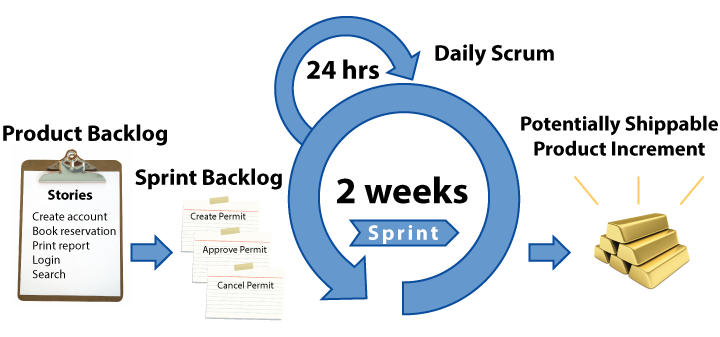
\includegraphics[width=5in,keepaspectratio]{scrum.png}
		\caption{ Scrum processes\protect\refstepcounter{footnote}\protect\footnotemark[\thefootnote]}
		
		
		\label{scrum-label}
	\end{figure}
	\footnotetext[\thefootnote]{Source: http://www.althea-groupe.com}
	Sprints can last from a few hours to a month (with a two-week preference). Each sprint has a goal and is associated with a list of features to achieve. Also each sprint begins with an estimate followed by operational planning, ends with a demonstration of what has been completed and helps to increase the business value of the product as shown in Figure \ref{scrum-label}. Before starting a new sprint, the team performs a retrospective: it analyzes what happened during this sprint, and improve for the next.
	\section*{Conclusion}
	\addcontentsline{toc}{section}{Conclusion}
	In this chapter, we have briefly presented the \textbf{``Anypli''} company and elucidated the field of study of our work. Then, an existing study was developed to describe the problematic in order to identify the deficiencies to be corrected.
	The next chapter will focus on the requirements.
	\chapter{Requirements}
	\section*{Introduction}
	\addcontentsline{toc}{section}{Introduction}
	In the previous chapter, we chose to adopt the Scrum methodology for designing our future system. In fact, Scrum is organized into three phases, the first of which is the planning and architecture phase (also known as sprint 0 in some books). This phase is the most important in the Scrum development cycle since it directly influences the success of sprints. and in particular the first.\par 
	The work done in this period of time leads to build a good vision of the product, identify the roles of users and clear the main features to produce the initial backlog and a first sprint planning. This phase will be the subject of this chapter where we start by capturing the different needs, identify the roles of the users and prepare our release plan.
	
	\section{Requirements}
	\subsection{Actors}
	\textbf{``Cake it up !''} includes two main actors and one secondary actor. They are divided into two categories web and mobile as shown in Table \ref{table-actors}.
	\\
	\newcolumntype{l}{>{\columncolor{LightCyan}}c}
	\begin{table}[H]
		\begin{center}
			\caption{\label{table-actors} List of actors.} 
			\captionsetup[table]{skip=10pt}
			\setlength\doublerulesep{0.5pt}
			\begin{tabular}{|l|p{5cm}|p{8cm}| } 
				\hline
				\rowcolor{LightCyan}
				& \textbf{Actor}   & \textbf{Role}                                                                                 \\
				\hline
				\multirow{3}{*}{\textbf{Web} }
				
				& Pastry manager   & He is the owner of the pastry, he is responsible for the managing of his own bakery.          \\
				\cline{2-3}
				& Administrator    & This is a secondary actor, he has access to all the data of both web and mobile applications. \\
				\hline
				\textbf{Mobile} & Customer/Visitor & He has only access to the mobile application.                                                 \\
				
				\hline
			\end{tabular}
		\end{center}
		
	\end{table}
	
	\subsection{Functional requirements}
	The Functional requirements are any requirement which specifies what the system should do.
	The application should be able to response to all the user’s needs:
	
	\begin{itemize}
		\item For the web application:
		\begin{itemize}
			\item  The administrator also known as the web master should be able to:
			\begin{itemize}
				\item Connect into his private space of the application,
				\item Manage reports,
				\item View statistics
				\item Activate/deactivate pastries,
				\item Block clients,
				\item Manage account,
				\item and also Receive notifications.
				
			\end{itemize}
			\item  The second actor which is the Bakery manager	or the pastry owner need to have access to the flowing functions: 
			\begin{itemize}
				\item Create an account,
				\item Connect,
				\item Manage his shop,
				\item Manage complains received from the clients,
				\item Manage orders,
				\item View statistics,
				\item Manage his own products,
				\item Manage personal events,
				\item Receive notifications.		
			\end{itemize}
		\end{itemize}
		\item As for the mobile application we can find two types of users:
		\begin{itemize}
			\item The visitor who also have multiple activities that has to be fulfilled, such as:
			\begin{itemize}
				\item The ability to create an account,
				\item To connect,
				\item Manage cart,
				\item Consult pastries and products.
			\end{itemize}
			\item Once the visitor connect his role changes to a customer, which will give him more advantages:
			\begin{itemize}
				\item he can manage his account,
				\item Manage orders,
				\item Create complains,
				\item Manage cart,
				\item Add reviews,
				\item Consult pastries and products,
				\item Create a personal order,
				\item Report a Bakery,
				\item Access to history of orders,
				\item Receive notifications,
				\item and rate a pastry shop
			\end{itemize}
			
			
		\end{itemize}
	\end{itemize}
	
	\subsection{Non-Functional requirements}
	Non-Functional requirements are any requirement which specifies how the system performs a certain function. They generally specify the system’s quality attributes or characteristics.
	\begin{itemize}
		\item Security: every account is secured by a encrypted password 
		\item Performance: quick response
		\item Reliability: fault tolerance
		\item Maintainability: easy to fix and evolve
		\item Availability: the application can be used anytime and anywhere
		
	\end{itemize}
	\section{Project management with SCRUM}
	\subsection{SCRUM}
	To manage the Scrum projects, team members use several techniques. One of these techniques, which is the most answered, is to create cards and paste them on a wall or a table visible to all members of the team. Another technique is to use an Excel file containing all the necessary information for sprints, user stories, estimates, and so on. This file must be shared in read and write (so that all members of the team can change it at any time).
	\subsection{SCRUM roles }
	Scrum defines three roles, which are:
	\begin{itemize}
		\item The Product Owner: The person with the product vision, usually an expert in the field.
		\item The Scrum Master (product manager): it is the person who must ensure the smooth running of the different sprints of the release, and who must imperatively master Scrum.
		\item Development Team: The team members who execute the work.
		
	\end{itemize}
	\section{Product Backlog}
	The backlog of the product is the most important artifact of Scrum, it is the set of functional or technical characteristics that constitute the desired product. These items can have a technical nature or can be user-centric e.g. in the form of user stories. The owner of the Scrum Product Backlog is the Scrum Product Owner. The Scrum Master, the Scrum Team and other Stakeholders contribute it to have a broad and complete To-Do list.\par
	Table \ref{table-backlog-product} summarizes the product backlog of our application.\par 
	\begin{table}[H]
		\begin{center}
			\captionsetup[table]{skip=10pt}
			\caption{\label{table-backlog-product} Product Backlog.}
			\setlength\doublerulesep{0.5pt}
			\begin{tabular}{|  p{1cm}|  p{4cm}|  p{1cm}| p{5cm}|  p{2cm}| p{2cm}|}
				\hline 
				\rowcolor{LightCyan}
				\textbf{ } & \textbf{Theme} & \textbf{ID} & \textbf{User story} & \textbf{Importance} & \textbf{Risk} 
				\\ \hline
				\multirow{2}{*}{\textbf{1} }
				&                        
				Authentification &                        
				1.1 &                        
				As an unauthorized User i want to create a new account.&                        
				High &                        
				Low
				\\
				\cline{3-6}
				&                        
				&                        
				1.2 &                        
				As an unauthorized User i want to login.&                        
				High &                        
				Low
				\\
				\cline{3-6}
				&                        
				&                        
				1.3 &                        
				As an authorized User i want to logout.&                        
				High &                        
				Low
				\\
				\cline{3-6}
				&                        
				&                        
				1.4 &                        
				As an unauthorized User i want to reset my password.&                        
				High &                        
				High
					\\
				\hline
				\multirow{2}{*}{\textbf{2} }
				&                        
				Manage account &                        
				2.1 &                        
				As an authorized user i want to edit my own account.&                        
				Medium &                        
				High
				\\
				\hline
				\multirow{2}{*}{\textbf{3} }
				&                        
				Manage pastries &                        
				3.1 &                        
				As a pastry owner i want to edit my own pastry.&                        
				High &                        
				High
				\\
				\cline{3-6}
				&                        
				&                        
				3.2 &                        
				As an Administrator i want to view the list of pastries.&                        
				High &                        
				Medium
				\\
				\cline{3-6}
				&                        
				&                        
				3.3 &                        
				As an Administrator i want to block a pastry.&                        
				Low &                        
				Low
				\\
				\cline{3-6}
				&                        
				&                        
				3.4 &                        
				As an Administrator i want activate or dis-activate a pastry.&                        
				Low &                        
				Low
				\\
				\cline{3-6}
				&                        
				&                        
				3.5 &                        
				As an client i want to view and search the list of activated pastries.&                        
				High &                        
				Low
					\\
				\cline{3-6}
				&                        
				&                        
				3.6 &                        
				As a pastry owner i want to dis-activate my own pastry if it is activated.&                        
				High &                        
				Low
				
				\\
				\hline
				
			\end{tabular}
			
		\end{center}
		
	\end{table}
	\begin{table}[H]
		\begin{center}
			\captionsetup[table]{skip=10pt}
			\setlength\doublerulesep{0.5pt}
			\begin{tabular}{|  p{1cm}|  p{4cm}|  p{1cm}| p{5cm}|  p{2cm}| p{2cm}|}
				\hline 
				\rowcolor{LightCyan}
				\textbf{ } & \textbf{Theme} & \textbf{ID} & \textbf{User story} & \textbf{Importance} & \textbf{Risk} 
				\\ \hline
				\multirow{2}{*}{\textbf{4} }
				&                        
				Manage products &                        
				4.1 &                        
				As a pastry owner i want to add a product.&                        
				High &                        
				High
				\\
				\cline{3-6}
				&                        
				&                        
				4.2 &                        
				As a pastry owner i want to edit a product.&                        
				High &                        
				High
				\\
				\cline{3-6}
				&                        
				&                        
				4.3 &                        
				As a pastry owner i want to view list of products.&                        
				High &                        
				Low
				\\
				\cline{3-6}
				&                        
				&                        
				4.4 &                        
				As a pastry owner i want to archive a product.&                        
				Low &                        
				Low
				
				\\ \hline
				\multirow{2}{*}{\textbf{5} }
				&                        
				Manage clients &                        
				5.1 &                        
				As an administrator i want to view list of all clients.&                        
				High &                        
				Low
				\\
				\cline{3-6}
				&                        
				&                        
				5.2 &                        
				As an administrator i want to block a client.&                        
				Low &                        
				Low
				\\
				\cline{3-6}
				&                        
				&                        
				5.3 &                        
				As a pastry owner i want to view list of my clients.&                        
				High &                        
				Low
				\\
				\hline
				\multirow{2}{*}{\textbf{6} }
				&                        
				Manage complains &                        
				6.1 &                        
				As a client i want to add a complain.&                        
				Medium &                        
				Low
				\\
				\cline{3-6}
				&                        
				&                        
				6.2 &                        
				As a client i want to view my list of complains.&                        
				Medium &                        
				Low
				\\
				\cline{3-6}
				&                        
				&                        
				6.2 &                        
				As a pastry owner i want to view the list of complains.&                        
				Medium &                        
				Low
				\\
				\cline{3-6}
				&                        
				&                        
				6.3 &                        
				As a pastry owner i want to reply to a complain..&                        
				Medium &                        
				Medium
				
				\\ \hline
					\multirow{2}{*}{\textbf{7} }
					&                        
				Manage Reports &                        
				7.1 &                        
				As a client i want to report a pastry.&                        
				Low &                        
				Low
				\\
				\cline{3-6}
				&                        
				&                        
				7.2 &                        
				As a pastry owner i want to report a client.&                        
				Low &                        
				Low
				\\
				\cline{3-6}
				&                        
				&                        
				7.3 &                        
				As an administrator i want to view list of reports.&                        
				Low &                        
				Low
				
				\\
				\hline
			\end{tabular}
			
		\end{center}
		
	\end{table}
	\begin{table}[H]
		\begin{center}
			\captionsetup[table]{skip=10pt}
			\setlength\doublerulesep{0.5pt}
			\begin{tabular}{|  p{1cm}|  p{4cm}|  p{1cm}| p{5cm}|  p{2cm}| p{2cm}|}
				\hline 
				\rowcolor{LightCyan}
				\textbf{ } & \textbf{Theme} & \textbf{ID} & \textbf{User story} & \textbf{Importance} & \textbf{Risk} 
				\\
				\hline
				\multirow{2}{*}{\textbf{8} }
				&                        
				Manage events &                        
				8.1 &                        
				As a pastry owner i want to add a personal event.&                        
				Low &                        
				Medium
				\\
				\cline{3-6}
				&                        
				&                        
				8.2 &                        
				As a pastry owner i want to view my calender.&                        
				Low &                        
				Low
					
				\\
				\hline
				\multirow{2}{*}{\textbf{9} }
				&                        
				Manage reviews &                        
				9.1 &                        
				As a client i want to add a review.&                        
				Low &                        
				Medium
				\\
				\cline{3-6}
				&                        
				&                        
				9.2 &                        
				As a pastry owner i want to view my pastry's reviews.&                        
				Low &                        
				Low
					
				\\
				\hline
				\multirow{2}{*}{\textbf{10} }
				&                        
				Manage ratings &                        
				10.1 &                        
				As a client i want to rate a pastry.&                        
				Low &                        
				Medium
				\\
				\cline{3-6}
				&                        
				&                        
				10.2 &                        
				As a pastry owner i want to view my pastry's rating.&                        
				Low &                        
				Low
			
			
				\\ \hline
				\multirow{2}{*}{\textbf{11} }
				&                        
				Statistics &                        
				11.1 &                        
				As an administrator or a pastry owner i want to view statistics.&                        
				Medium &                        
				Low
				
				\\ \hline
				\multirow{2}{*}{\textbf{12} }
				&                        
				Manage cart &                        
				12.1 &                        
				As a client i want to edit my cart.&                        
				High &                        
				High
				\\
				\cline{3-6}
				&                        
				&                        
				12.2 &                        
				As a client i want to view my cart.&                        
				High &                        
				Low
					\\ \hline
				\multirow{2}{*}{\textbf{13} }
				&                        
				Manage orders &                        
				13.1 &                        
				As a client i want to pass an order.&                        
				High &                        
				High
				\\
				\cline{3-6}
				&                        
				&                        
				13.2 &                        
				As a client i want to view my own orders.&                        
				High &                        
				Low
				\\
				\cline{3-6}
				&                        
				&                        
				13.3 &                        
				As a pastry owner i want to view orders.&                        
				High &                        
				Low
				\\
				\cline{3-6}
				&                        
				&                        
				13.4 &                        
				As a pastry owner i want to change the state of an order.&                        
				High &                        
				Medium
				
				\\
				\hline
				\multirow{2}{*}{\textbf{14} }
				&                        
				Manage personal orders &                        
				14.1 &                        
				As a client i want to add a personal order.&                        
				High &                        
				High
				\\
				\cline{3-6}
				&                        
				&                        
				14.2 &                        
				As a client i want to view my list of personal orders.&                        
				High &                        
				Low
				
				
				
				\\
				\hline
			\end{tabular}
			
		\end{center}
	\end{table}
	\clearpage
	\section{General use case diagram}
	The purpose of a \ac{ucd}\footnote{A use case diagram can summarize the details of your system's users (also known as actors) and their interactions with the system} in \ac{uml}\footnote{The OMG's Unified Modeling Language™ (UML®) helps you specify, visualize, and document models of software systems, including their structure and design, in a way that meets all of these requirements} is to demonstrate the different ways that a user might interact with a system.\\
	A use case helps represent: 
	
	\begin{itemize}
		\item 	Scenarios in which your system or application interacts with people, organizations, or external systems
		\item 	Goals that your system or application helps those entities (known as actors) achieve
		\item  	The scope of your system
	\end{itemize}
	
	\subsection{Use case: web}
	This section will give a detailed description of the general and detailed use cases that exists in the web application.
	\begin{figure}[H]
		\vspace*{1cm}
		
		\centering
		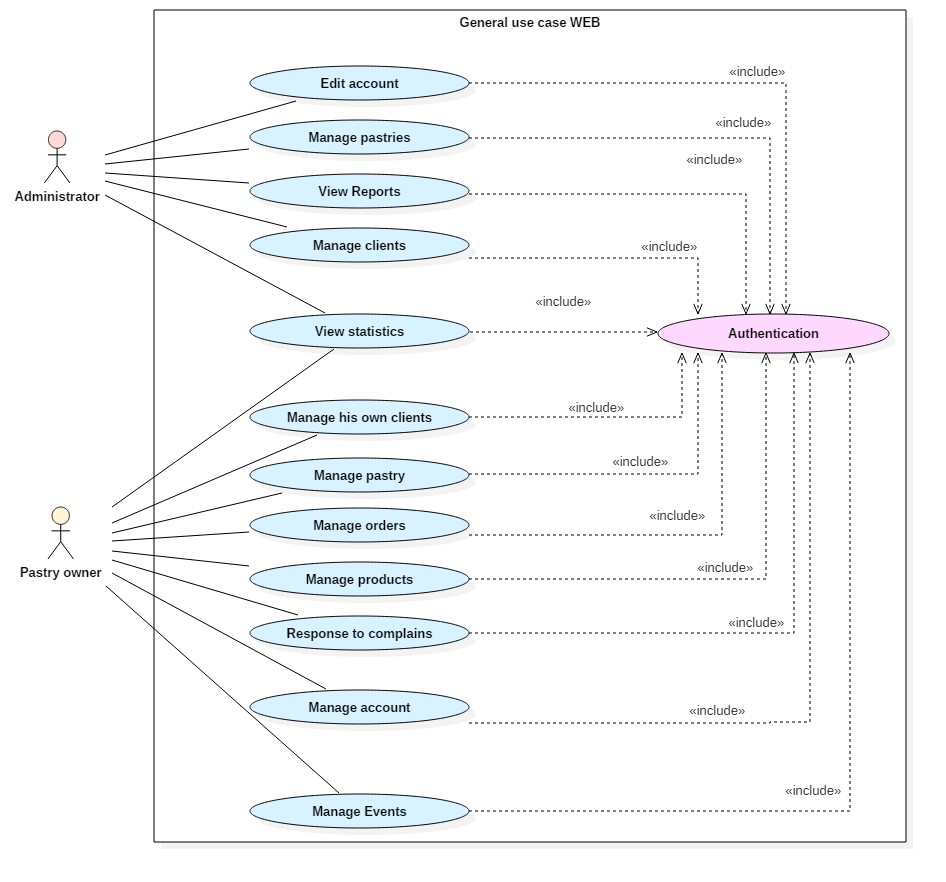
\includegraphics[width=7in,keepaspectratio]{usecaseWeb.png}
		\caption{General use case: Web}
		\label{user-case-web}
	\end{figure}
	
	\begin{table}[H]
		\begin{center}
			\caption{\label{user-case-web-explanation} General use case web explanation} 
			\captionsetup[table]{skip=10pt}
			\setlength\doublerulesep{0.5pt}
			\begin{tabular}{|l|p{5cm}|p{8cm}| } 
				\hline\hline
				\rowcolor{LightCyan}
				& \textbf{Use case}      & \textbf{Explanation}                                                                                                                                \\
				\hline
				\hline
				\multirow{5}{*}{\textbf{Administrator} }
				
				& Edit account           & The administrator has access to his own private account where he can edit his personal information,                                                 \\
				\cline{2-3}
				& Manage pastries        & He can also view the list of all the pastries and manage them but with limits,                                                                      \\
				\cline{2-3}
				& View Reports           & Viewing the reports is also an option, a report can be send from a client or a pastry,                                                              \\
				\cline{2-3}
				& Manage clients         & Managing the clients is one of the Administrator's tasks.                                                                                           \\
				
				\hline
				\hline
				\multirow{5}{*}{\textbf{Patsy owner} }
				& Manage his own clients & The second user which is the pastry's owner have access to the list of his clients (the ones who made at least one order with them),                
				\\
				\cline{2-3}
				& Manage pastry          & He can view the information of his pastry and edit or deactivate it,                                                                                
				\\
				\cline{2-3}
				& Manage orders          & All the orders made by a client can be seen by the pastry's owner, and he has multiple actions he can use on an order(accept, refuse, cancel, ...), 
				\\
				\cline{2-3}
				& Manage products        & Every pastry has a list of products that are created and managed by the pastry's owner,                                                             
				\\
				\cline{2-3}
				& Response to complains  & The complains made by the clients are only visible to this user, he has the ability to response to these complain by a message,                     
				\\
				\cline{2-3}
				& Manage account         & The pastry's owner have access to his own information (email, password)                                                                             \\
				\cline{2-3}
				& Manage events          & The pastry's owner have a secondary option which is handling his private calendar                                                                   \\
				\hline
			\end{tabular}
		\end{center}
		
		
	\end{table}
	
	
	\subsection{Use case: Mobile}
	\begin{figure}[H]
		\centering
		\includegraphics[width=7in,keepaspectratio]{UseCasemobile.png}
		\caption{General use case: Mobile}
		\label{user-case-mobile}
	\end{figure}
	\begin{table}[H]
		\begin{center}
			\caption{\label{user-case-mobile-explanation} General use case mobile explanation} 
			\captionsetup[table]{skip=10pt}
			\setlength\doublerulesep{0.5pt}
			\begin{tabular}{|l|p{5cm}|p{8cm}| } 
				\hline\hline
				\rowcolor{LightCyan}
				& \textbf{Use case}      & \textbf{Explanation}                                                                                                                                \\
				\hline
				\hline
				\multirow{5}{*}{\textbf{Administrator} }
				
				& Edit account           & The administrator has access to his own private account where he can edit his personal information,                                                 \\
				\cline{2-3}
				& Manage pastries        & He can also view the list of all the pastries and manage them but with limits,                                                                      \\
				\cline{2-3}
				& View Reports           & Viewing the reports is also an option, a report can be send from a client or a pastry,                                                              \\
				\cline{2-3}
				& Manage clients         & Managing the clients is one of the Administrator's tasks.                                                                                           \\
				
				\hline
				\hline
				\multirow{5}{*}{\textbf{Patsy owner} }
				& Manage his own clients & The second user which is the pastry's owner have access to the list of his clients (the ones who made at least one order with them),                
				\\
				\cline{2-3}
				& Manage pastry          & He can view the information of his pastry and edit or deactivate it,                                                                                
				\\
				\cline{2-3}
				& Manage orders          & All the orders made by a client can be seen by the pastry's owner, and he has multiple actions he can use on an order(accept, refuse, cancel, ...), 
				\\
				\cline{2-3}
				& Manage products        & Every pastry has a list of products that are created and managed by the pastry's owner,                                                             
				\\
				\cline{2-3}
				& Response to complains  & The complains made by the clients are only visible to this user, he has the ability to response to these complain by a message,                     
				\\
				\cline{2-3}
				& Manage account         & The pastry's owner have access to his own information (email, password)                                                                             \\
				\cline{2-3}
				& Manage events          & The pastry's owner have a secondary option which is handling his private calendar                                                                   \\
				\hline
			\end{tabular}
		\end{center}
		
		
	\end{table}
	\section{Conceptual Data Modeling}
	\subsection{Data dictionary}
	Following the conceptual modeling of UML, all the data mentioned in the dictionary are organized according to classes.\par 
	Classes are the basic modules of object-oriented programming. It is a formal description of a set of objects with common semantics and features.
	\begin{table}[H]
		\begin{center}
			\captionsetup[table]{skip=10pt}
			\caption{Pastry class}
			\setlength\doublerulesep{0.5pt}
			
			\begin{tabular}{|  p{5cm}|  p{6cm}|  p{4cm}|}
				\rowcolor{LightCyan}
				
				\hline
				\multicolumn{3}{c}{Pastry class}\\
				\hline 
				\textbf{Code} & \textbf{Meaning} & \textbf{Data type} 
				\\ \hline
				
				name &                        
				The name of the pastry &                        
				String                     
				
				\\ \hline
				
				description &                        
				the description of the pastry &                        
				String   
				\\ \hline
				
				mail &                        
				the mail address of the pastry &                        
				String 
				\\ \hline
				
				web\_site &                        
				the web site of the pastry &                        
				String   
				\\ \hline
				
				date\_open &                        
				the opening date of the pastry &                        
				DateTime  
				\\ \hline
				
				logo &                        
				the logo of the pastry &                        
				String  
				\\ \hline
				
				delivery &                        
				The pastry does deliveries or not &                        
				Boolean
				\\ \hline
				
				isActive &                        
				The pastry is activated or not &                        
				Boolean
				\\ \hline
				
				isBlocked &                        
				The pastry is blocked or not &                        
				Boolean      
				
				\\ \hline
				
			\end{tabular}
			
		\end{center}
	\end{table}
	\begin{table}[H]
		\begin{center}
			\captionsetup[table]{skip=10pt}
			\caption{User class}
			\setlength\doublerulesep{0.5pt}
			
			\begin{tabular}{|  p{5cm}|  p{6cm}|  p{4cm}|}
				\rowcolor{LightCyan}
				
				\hline
				\multicolumn{3}{c}{User class}\\
				\hline 
				\textbf{Code} & \textbf{Meanning} & \textbf{Data type} 
				\\ \hline
				
				email &                        
				The email of the user &                        
				String                     
				
				\\ \hline
				
				password &                        
				the password of the pastry &                        
				String   
				
				\\ \hline
				
			\end{tabular}
			
		\end{center}
	\end{table}
	\begin{table}[H]
		\begin{center}
			\captionsetup[table]{skip=10pt}
			\caption{Product class}
			\setlength\doublerulesep{0.5pt}
			
			\begin{tabular}{|  p{5cm}|  p{6cm}|  p{4cm}|}
				\rowcolor{LightCyan}
				
				\hline
				\multicolumn{3}{c}{Product class}\\
				\hline 
				\textbf{Code} & \textbf{Meanning} & \textbf{Data type} 
				\\ \hline
				
				ref &                        
				A unique reference for the product &                        
				String                     
				
				\\ \hline
				
				name &                        
				The product's name &                        
				String   
				\\ \hline
				
				description &                        
				The description of the product &                        
				String 
				\\ \hline
				
				price &                        
				The product's price &                        
				Decimal   
				\\ \hline
				
				stock &                        
				Quantity of products in stock &                        
				Integer  
				\\ \hline
				
				image &                        
				The image of the product &                        
				String
				
				\\ \hline
				
			\end{tabular}
			
		\end{center}
	\end{table}
	\begin{table}[H]
		\begin{center}
			\captionsetup[table]{skip=10pt}
			\caption{Order class}
			\setlength\doublerulesep{0.5pt}
			
			\begin{tabular}{|  p{5cm}|  p{6cm}|  p{4cm}|}
				\rowcolor{LightCyan}
				
				\hline
				\multicolumn{3}{c}{Order class}\\
				\hline 
				\textbf{Code} & \textbf{Meaning} & \textbf{Data type} 
				\\ \hline
				
				quantity &                        
				the number of products in the order &                        
				Integer                     
				
				\\ \hline
				
				description &                        
				The description of the order if it exist &                        
				String  
				\\ \hline
				
				status &                        
				To describe in what state is the product (waiting, done, canceled ...) &                        
				Integer
				\\ \hline
				
				total\_amount &                        
				The price of the whole order &                        
				Decimal
				\\ \hline
				
				date\_order &                        
				The date to deliver the order &                        
				DateTime    
				
				\\ \hline
				
			\end{tabular}
			
		\end{center}
	\end{table}
	\begin{table}[H]
		\begin{center}
			\captionsetup[table]{skip=10pt}
			\caption{Review class}
			\setlength\doublerulesep{0.5pt}
			
			\begin{tabular}{|  p{5cm}|  p{6cm}|  p{4cm}|}
				\rowcolor{LightCyan}
				
				\hline
				\multicolumn{3}{c}{Review class}\\
				\hline 
				\textbf{Code} & \textbf{Meanning} & \textbf{Data type} 
				\\ \hline
				
				content &                        
				The comment added with the review &                        
				String  
				\\ \hline
				
				date\_creation &                        
				The date when the review was created &                        
				DateTime                    
				
				\\ \hline
				
				
			\end{tabular}
			
		\end{center}
	\end{table}
	\begin{table}[H]
		\begin{center}
			\captionsetup[table]{skip=10pt}
			\caption{Complain class}
			\setlength\doublerulesep{0.5pt}
			
			\begin{tabular}{|  p{5cm}|  p{6cm}|  p{4cm}|}
				\rowcolor{LightCyan}
				
				\hline
				\multicolumn{3}{c}{Complain class}\\
				\hline 
				\textbf{Code} & \textbf{Meaning} & \textbf{Data type} 
				\\ \hline
				
				description &                        
				Every complain has a description &                        
				String  
				\\ \hline
				
				date\_creation &                        
				The date when the complain was created &                        
				DateTime                    
				
				\\ \hline
				
				
			\end{tabular}
			
		\end{center}
	\end{table}
	\begin{table}[H]
		\begin{center}
			\captionsetup[table]{skip=10pt}
			\caption{Schedule class}
			\setlength\doublerulesep{0.5pt}
			
			\begin{tabular}{|  p{5cm}|  p{6cm}|  p{4cm}|}
				\rowcolor{LightCyan}
				
				\hline
				\multicolumn{3}{c}{Schedule class}\\
				\hline 
				\textbf{Code} & \textbf{Meaning} & \textbf{Data type} 
				\\ \hline
				
				day &                        
				The day of the week &                        
				String  
				\\ \hline
				
				open\_time &                        
				Opennigng time &                        
				Time 
				\\ \hline
				
				close\_time &                        
				Closing time &                        
				Time                   
				
				\\ \hline
				
				
			\end{tabular}
			
		\end{center}
	\end{table}
	\begin{table}[H]
		\begin{center}
			\captionsetup[table]{skip=10pt}
			\caption{event class}
			\setlength\doublerulesep{0.5pt}
			
			\begin{tabular}{|  p{5cm}|  p{6cm}|  p{4cm}|}
				\rowcolor{LightCyan}
				
				\hline
				\multicolumn{3}{c}{event class}\\
				\hline 
				\textbf{Code} & \textbf{Meaning} & \textbf{Data type} 
				\\ \hline
				
				title &                        
				The title of the event &                        
				String  
				\\ \hline
				
				date &                        
				The date of the event &                        
				Date            
				
				\\ \hline
				
				
			\end{tabular}
			
		\end{center}
	\end{table}
	\begin{table}[H]
		\begin{center}
			\captionsetup[table]{skip=10pt}
			\caption{Address class}
			\setlength\doublerulesep{0.5pt}
			
			\begin{tabular}{|  p{5cm}|  p{6cm}|  p{4cm}|}
				\rowcolor{LightCyan}
				
				\hline
				\multicolumn{3}{c}{Address class}\\
				\hline 
				\textbf{Code} & \textbf{Meaning} & \textbf{Data type} 
				\\ \hline
				
				longitude &                        
				The longitude of the address &                        
				Decimal  
				\\ \hline
				
				latitude &                        
				The latitude of the address &                        
				Decimal            
				
				\\ \hline
				
				
			\end{tabular}
			
		\end{center}
	\end{table}
	\begin{table}[H]
		\begin{center}
			\captionsetup[table]{skip=10pt}
			\caption{Personal\_product class}
			\setlength\doublerulesep{0.5pt}
			
			\begin{tabular}{|  p{5cm}|  p{6cm}|  p{4cm}|}
				\rowcolor{LightCyan}
				
				\hline
				\multicolumn{3}{c}{Personal\_product class}\\
				\hline 
				\textbf{Code} & \textbf{Meaning} & \textbf{Data type} 
				\\ \hline
				
				allergy &                        
				List of allergies the client might have &                        
				String  
				\\ \hline
				
				plus &                        
				A comment added by the client &                        
				Decimal            
				
				\\ \hline
				
				
			\end{tabular}
			
		\end{center}
	\end{table}
	\subsection{Class diagram}
	Class diagrams are one of the most useful types of diagrams in \ac{uml} \cite{umlBook} as they clearly map out the structure of a particular system by modeling its classes, attributes, operations, and relationships between objects.
	
	
	
	\vspace*{2cm}
	\begin{figure}[H]
		\centering
		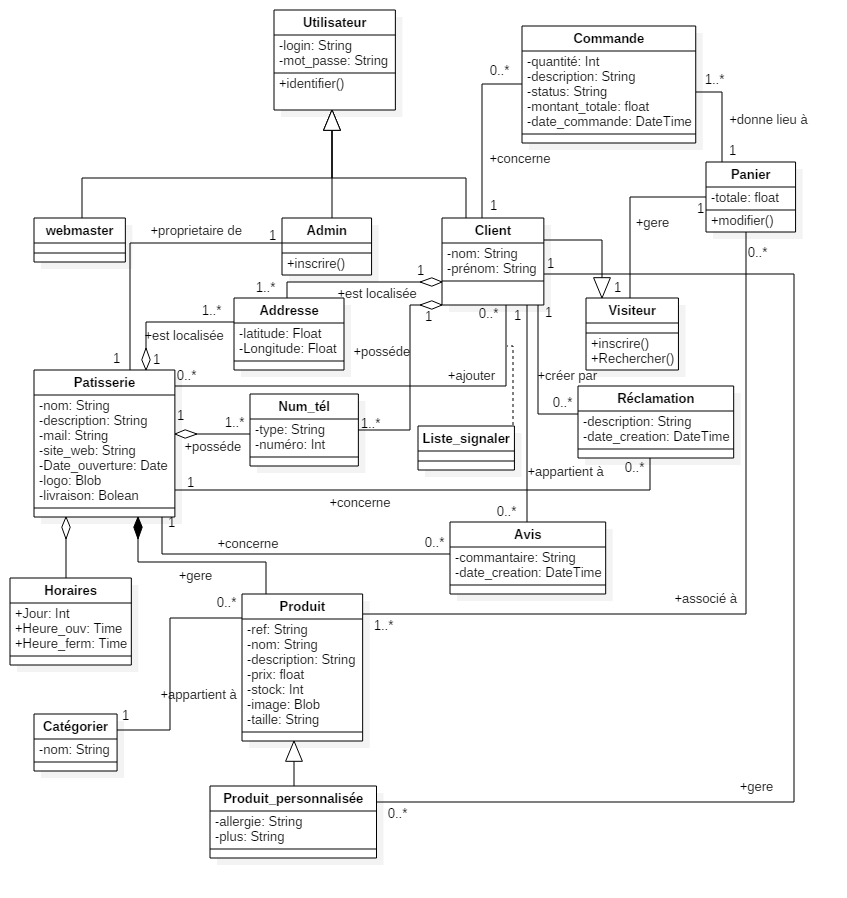
\includegraphics[width=7.7in,keepaspectratio]{class.png}
		\caption{Class Diagram}
	\end{figure}
	
	\begin{table}[H]
		\begin{center}
			
			\caption{\label{Class_explanation} Class diagram explanation}
			\captionsetup[table]{skip=10pt}
			\setlength\doublerulesep{0.5pt}
			\begin{tabular}{| l | p{12cm} |}
				\hline \hline\hline
				\rowcolor{LightCyan}
				\textbf{ Entities} & \textbf{Definition} \\ \hline\hline\hline
				User               &                     
				\vtop{\hbox{\strut The user can be the administrator, the pastry owner, the visitor oe the client}}
				
				\\ \hline
				Pastry owner      &                     
				\vtop{\hbox{\strut The person who manges the pastry.}}
				
				\\ \hline
				Administrator       &                     
				\vtop{\hbox{\strut The person who manage the application.}}
				\\
				\hline
				Client             &                     
				\vtop{\hbox{\strut The person who will be passing orders.}}
				\\ \hline
				Visitor             &                     
				\vtop{\hbox{\strut Is a client who does not have an account}}
				\\ \hline
				Pastry              &                     
				\vtop{\hbox{\strut The pastry added by the owner}}
				\\ \hline
				History        &                     
				\vtop{\hbox{\strut Any order or complain or a block done by a client is saved in this table.}}
				\\ \hline
				Review               &                     
				\vtop{\hbox{\strut The client have an option a write a review about a pastry.}}
				\\ \hline
				Product               &                     
				\vtop{\hbox{\strut Every pastry has a number of products.}}
				\\ \hline
				Event         &                     
				\vtop{\hbox{\strut An event can be created by a pastry owner.}}
				\\ \hline
				Favorites    &                     
				\vtop{\hbox{\strut The client can add a pastry to his favorite list}}
				\\ \hline
				Address           &                     
				\vtop{\hbox{\strut Both the client and a pastry have an address.}}
				\\ \hline
				Personal\_products             &                     
				\vtop{\hbox{\strut The client can create his own personal product.}}
				\\ \hline
				Complains              &                     
				\vtop{\hbox{\strut A complain can be send from a client to a pastry owner.}}
			
				
				
				
			\end{tabular}
			
		\end{center}
		
	\end{table}
\begin{table}[H]
	\begin{center}
		
		\setlength\doublerulesep{0.5pt}
		\begin{tabular}{| l | p{12cm} |}
			\hline 
			Cart           &                     
			\vtop{\hbox{\strut Is where the orders are saved.}}
			\\ \hline
			Category           &                     
			\vtop{\hbox{\strut Each product belongs to a specific category.}}
			\\ \hline
			Schedule           &                     
			\vtop{\hbox{\strut The pastry have an opening and closing time.}}
			\\ \hline
			Report           &                     
			\vtop{\hbox{\strut Both pastry owners and clients can report each other.}}
			\\ \hline
			Phone           &                     
			\vtop{\hbox{\strut A phone number can belong to a pastry or a client.}}
			\\ \hline
			
			
			
		\end{tabular}
		
	\end{center}
	
\end{table}
	\section{Sprint Planning}
	The planning stage is very important for better organization and management of the project.
	\begin{table}[H]
		\begin{center}
			\captionsetup[table]{skip=10pt}
			\caption{Sprint planning}
			\setlength\doublerulesep{0.5pt}
			
			\begin{tabular}{|  p{5cm}|  p{5cm}|  p{5cm}|}
				\rowcolor{LightCyan}
				
				\hline 
				\textbf{Release 1} & \textbf{Release 2} & \textbf{Release 3} 
				\\ \hline
				
				18 February - 22 March &                        
				23 March - 05 April &                        
				06 April - 31 May  
				\\ \hline
				\vtop{\hbox{\strut Authentication}\hbox{\strut Manage account}\hbox{\strut Manage pastries}\hbox{\strut Manage products}}				
				&             
				\vtop{\hbox{\strut Manage clients}\hbox{\strut Manage Complains}\hbox{\strut Manage reports}\hbox{\strut Manage events}}  
				&                        
				\vtop{\hbox{\strut Manage reviews}
					\hbox{\strut Manage rating}
					\hbox{\strut Statistics}
				\hbox{\strut Manage cart}
				\hbox{\strut Mange orders}
				\hbox{\strut Manage Personal orders}}  
				
				\\ \hline
				
				
			\end{tabular}
			
		\end{center}
	\end{table}
	\section*{Conclusion}
	\addcontentsline{toc}{section}{Conclusion}
	This chapter allowed us to cover the different functional and non-functional needs of the actors of our application. We provided a representation of a use case diagram for actors reacting with the application and the sprint planning. The next chapter will deal with the realase 1.
	\chapter{Project Initialization}
	\section*{Introduction}
	\addcontentsline{toc}{section}{Introduction}
	We dedicate this chapter to initializing the project and setting up the development environment. The architecture as well as the software and technologies will be explained
	thereafter.
	\section{Choice of the architecture}
	The definition of the application architecture is an important step in the design process. It depends on a number of factors including performance requirements, prospects and scalability. Figure \ref{label-archi} illustrates a representation of the software architecture of the project.\par 
	The choice of the architecture of the application is considered as an important step
	in the process of making the application. Our application
	consists of three parts that are, the front-end part, the back-end part and the mobile app. The first part
	is done with the VueJS framework which consumes the REST API implied by the second
	part that is done with Laravel, Also the the third part consumes the REST API implied by the second part also.\par
	
	We chose to split the application architecture into two major parts,
	one layer as a the back-office that contain Laravel app and VueJS app, and the other part as the front-office contains the Android mobile application which also uses the Laravel app as a backe-end. 
	That of Laravel communicates
	with the MYSQL database using the ELOQUENT
	\ac{orm} that is to say everything in the database has a
	representation as manipulable objects to simplify access and operations
	On the base.
	With the Eloquent principle, a table is represented by a PHP class that extends the class
	Model. And the controller contains the logic concerning the actions performed by the user. It
	defines all the methods that represent the actions.
	In the Laravel part (Server side), we have implemented our API. The latter will specify all the logic that will be exploited by
	the VueJS part and the mobile Android app (Client side) using AXIOS in VueJS and Retrofit in Android. Quite simply, we tell them the method
	HTTP that we would like to use (eg GET / POST / etc.) and to which URL the request
	must be called.\par
	Axios is a popular HTTP client based on promises that sports an API `a
	use. It allows you to make HTTP requests to retrieve or save data that
	is one of the tasks that a client-side JavaScript application will need to perform.
	As well as Retrofit for the Android Rest client.\par
	
	In the
	VueJS part, we chose to use the VUEX State Management Library whose purpose
	to manage the state of the components of our application, and to facilitate their sharing.
	it separates the logic within the application to ensure better structuring and maintenance.
	\par

All these elements are grouped in the figure: \ref{label-archi} store of Vuex. The possibility of spreading
the state in several modules allows to manage several different states in the single store of
the application. For the android part, we have decided to go with MVP along with Retrofit.\par
\begin{figure}[H]
	\centering
	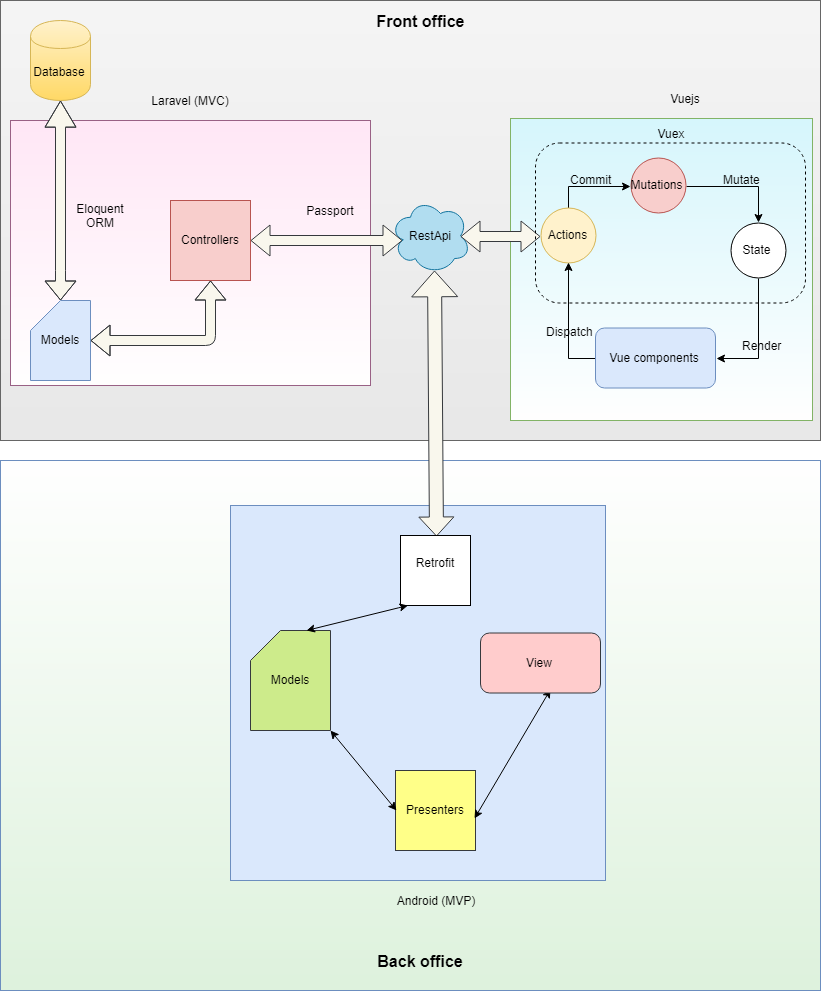
\includegraphics[width=5.5in,height=4.9in]{archi.png}
	\caption{Project architecture}
	\label{label-archi}
\end{figure}
 We will be explaining each and every design pattern used in this application:\par
\textbf{MVC}: This pattern was used for the back-end of the application, this pattern is actually used in Laravel which we will be using to create our APIs. MVC stands for Model-View-Controller as shown in Figure \ref{mvc}. \cite{mvc}\par 
\begin{itemize}
	\item \textbf{Model:} is the object carrying the data.
	\item \textbf{View:} the data in the model will be visible to the user via this pasrt.
	\item \textbf{Controller:} as for the controller is where we can find all the updates done on the model and sends them to the view.
\end{itemize}
\begin{figure}[H]
	\centering
	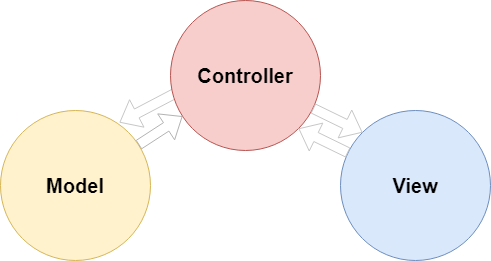
\includegraphics[width=4in,keepaspectratio]{mvc_pattern.png}
	\caption{MVC pattern}
	\label{mvc}
\end{figure}
\textbf{MVP}: For the android application we decided on using the MVP pattern to make our code cleaner and easier to understand. \par 
\begin{itemize}
	\item \textbf{Model:} Model is where the business logic and application data is stored.
	\item \textbf{View:} View is basically a passive interface cum UI which is responsible for routing user’s action to the presenter. In Android, View can be your Activity, fragment or RecyclerView Adapters.
	\item \textbf{Presenter:} Is the middleman or mediator between View and Model which hold responsibilities of everything which has to deal with presentation logic in your application.
\end{itemize}
\begin{figure}[H]
	\centering
	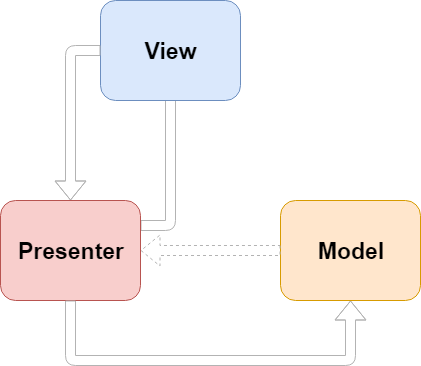
\includegraphics[width=4in,keepaspectratio]{mvp-patern.png}
	\caption{MVP pattern}
	\label{mvp}
\end{figure}
\textbf{MVVM}:The MVVM design pattern (model, view, view-style) is a derivative of the MVC design model. The principle of this design pattern is to separate into three layers (model, view, view-style) where the view always receives the actions of the user and only interacts with the ViewModel, and the model communicates with the server and notifies the View-Model of the changes made.\cite{Mvvm} \par 
\begin{itemize}
	\item \textbf{Model:} The model contains the data. Typically, this data comes from a database or an external service such as an API.
	\item \textbf{View (Vue):} he view corresponds to what is displayed (the web interface). The view contains the different graphic components (buttons, links, lists) as well as the text.
	\item \textbf{ViewModel (Model View):}  This component is the link between the model and the view. It takes care of managing data links and eventual conversions. This is where the binding comes in.
\end{itemize}
\begin{figure}[H]
	\centering
	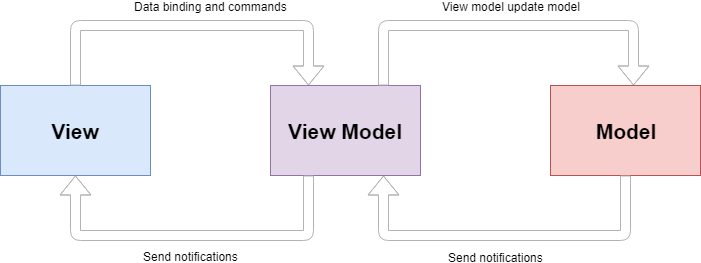
\includegraphics[width=6in,keepaspectratio]{mvvm-pettern.png}
	\caption{MVVM pattern}
	\label{mvvm}
\end{figure}

	
	\section{Programming languages}
	\subsection{Kotlin}
	\begin{wrapfigure}{L}{0.2\linewidth}
		\centering
		
\includegraphics[width=0.8in]{kotlin-logo.png}	
	\end{wrapfigure}
	We decided on using \textbf{``kotlin''} as an Android development language, seen it is the a perfect fit and considering the multiple advantages \textbf{``Kotlin''} has to offer.\par 
	\textbf{``Kotlin''} is the new open source programming language supported by Google. Its main goal is to improve the productivity of developers, while remaining compatible with the existing code. It is an object-oriented and functional programming language that can also be called a multi-paradigm language.\cite{kotlinbook}\par 
	As we can see in Figure \ref{kotlin-label}, \textbf{``Kotlin''} has experienced strong growth in Android application development since May, after Google announced its official support in Android Studio. This is revealed by the Realm barometer, as part of its latest quarterly report.
	\begin{figure}[H]
		\centering
		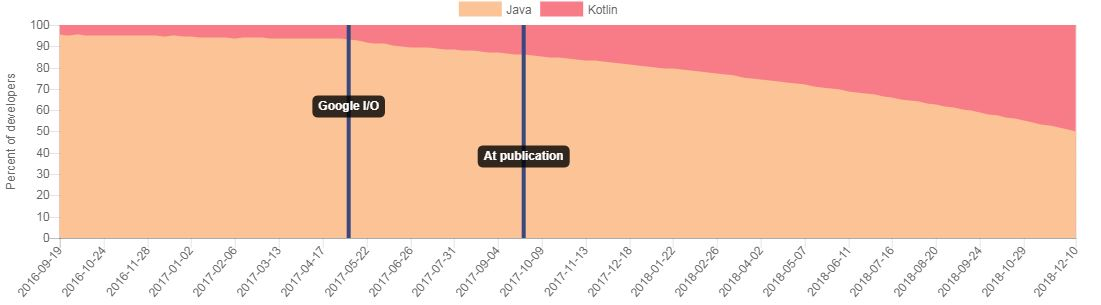
\includegraphics[width=7in,keepaspectratio]{kotlinjava.jpg}
		\caption{ Kotlin vs Java\protect\refstepcounter{footnote}\protect\footnotemark[\thefootnote]}
		
		\label{kotlin-label}
	\end{figure}
	\footnotetext[\thefootnote]{Source: Rapport Realm}
	\subsection{PHP}
	\begin{wrapfigure}{L}{0.2\linewidth}
		\centering
		
\includegraphics[width=0.8in]{PHP-logo.png}	
	\end{wrapfigure}
	As for backend it is natural that we will be working with \textbf{``\ac{php}''} since we chose Laravel as our backend framework. \cite{phpbook}\par 
	\textbf{``PHP''} is a server scripting language, specially designed for the development of web applications. It can be easily integrated with HTML. \par 
	It is common for this language to be associated with a database, such as My\ac{sql}. Executed on the server side there is no need for visitors to have particular software or plugins.
	\subsection{JavaScript}
	\begin{wrapfigure}{L}{0.2\linewidth}
		\centering
		
\includegraphics[width=0.8in]{JavaScript-logo.png}	
	\end{wrapfigure}
	We gonna be using Vuejs ergo \textbf{``JavaScript''} will be one of the programming languages we are using.\par 
	Javascript is an object-oriented scripting language mainly used in HTML pages. Unlike server languages that run on the site, \textbf{``JavaScript''} is executed on the user's computer by the browser itself. Thus, this language allows interaction with the user according to his actions.
	\section{Used technologies and frameworks}
	
	\subsection{Android}
	\begin{wrapfigure}{L}{0.2\linewidth}
		\centering
		
\includegraphics[width=0.8in]{android-logo.jpg}	
	\end{wrapfigure}
	\textbf{``Android''} is a mobile Operating \ac{os} developed by GOOGLE, Written primarily in Java and based on the Linux operating system~\cite{phillips2013android}.\par
	Native Android apps are developed using the Java programming language, and can easily be ported to other mobile operating systems like Blackberry, Symbian and Ubuntu.\par
	\textit{``The Android platform enables device makers to compete and innovate. App developers can reach huge audiences and build strong businesses. Consumers now have unprecedented choice in devices, at ever-lower prices.''}-Hiroshi Lockheimer, SVP, Android, Chrome \ac{os} and Play.
	\subsubsection*{Retrofit Android}
	\textbf{``Retrofit''} is type-safe REST client for Android and Java which aims to make it easier to consume Representational State Transfer (\ac{rest}ful) web services. \par 
	It will save our development time, And also we can keep our code in developer friendly. Retrofit has given almost all the \ac{api}'s to make server call and to receive response.

	\subsection{Laravel}
	\begin{wrapfigure}{L}{0.2\linewidth}
		\centering
		
\includegraphics[width=0.8in]{LaravelLogo.png}
	\end{wrapfigure}
	\textbf{``Laravel''} is a framework that has existed since 2011 but has exploded recently and seems to attract a lot of developers, is a PHP framework that offers tools to build a web application. Laravel's creator, Taylor Otwel, has simply grouped together the best libraries for every feature needed to create a website. \cite{laravelBook}
	\subsection{VueJS}
	\begin{wrapfigure}{L}{0.2\linewidth}
		\centering
		
\includegraphics[width=0.8in]{vue-logo.png}	
	\end{wrapfigure}
	\textbf{``VueJS''} was our chose for the front end of the we application, since it is Flexible and easy to use. \cite{vuejsbook}\par 
	\textbf{``VueJS''} is a JavaScript UI library. The core library is focused on the view layer only, and is easy to pick up and integrate with other libraries or existing projects. On the other hand, Vue is also perfectly capable of powering sophisticated Single-Page Applications when used in combination with modern tooling and supporting libraries. 
	\par 
	When comparing it with its competitors, including Angular, React, Ember, Aurelia, etc., Vue boasts of beating some of them in certain aspects. These aspects include simple \ac{api}, size, performance, learning curve, etc.
	\clearpage
	\subsubsection*{Vuetify}
	\begin{wrapfigure}{L}{0.2\linewidth}
		\centering
		
\includegraphics[width=0.8in]{vuetify-logo.png}	
		
	\end{wrapfigure}
	We can find multiple frameworks hat can be used with VueJs but we decided on one which is   \textbf{``Vuetify''}.\par 
	\textbf{``Vuetify''} is a progressive framework that attempts to push web development to the next level. It complies with the Material Design specification. This means the core features of both Vue and Material will be available by default and can be improved by both communities. In addition, Vuetify offers:
	\begin{itemize}
		\item Compatibility with Vue \ac{cli}-3 and \ac{rtl} 
		\item Templates for various frameworks (Cordova, webpack, etc.)
		\item Internationalization
		\item  \ac{ssr} and  \ac{pwa} 
		
	\end{itemize}
	\subsubsection*{Vuex}
	\begin{wrapfigure}{L}{0.2\linewidth}
		\centering
		
\includegraphics[width=0.8in]{vuex-logo.png}	
		
	\end{wrapfigure}
	\textbf{``Vuex''} is our chose to use as a state management pattern and library for Vuejs. It serves as a centralized store for all the components in an application, with rules ensuring that the state can only be mutated in a predictable fashion.\par 
	It helps us deal with shared state management with the cost of more concepts and boilerplate. It's a trade-off between short term and long term productivity.\par
	As showing in Figure \ref{label-vuex} it is a self-contained app with the following parts:
	\begin{itemize}
		\item The state, the source of truth that drives our app
		\item The view, a declarative mapping of the state
		\item The actions, the possible ways the state could change in reaction to user inputs from the view.
		
	\end{itemize}
	\begin{figure}[H]
		\centering
		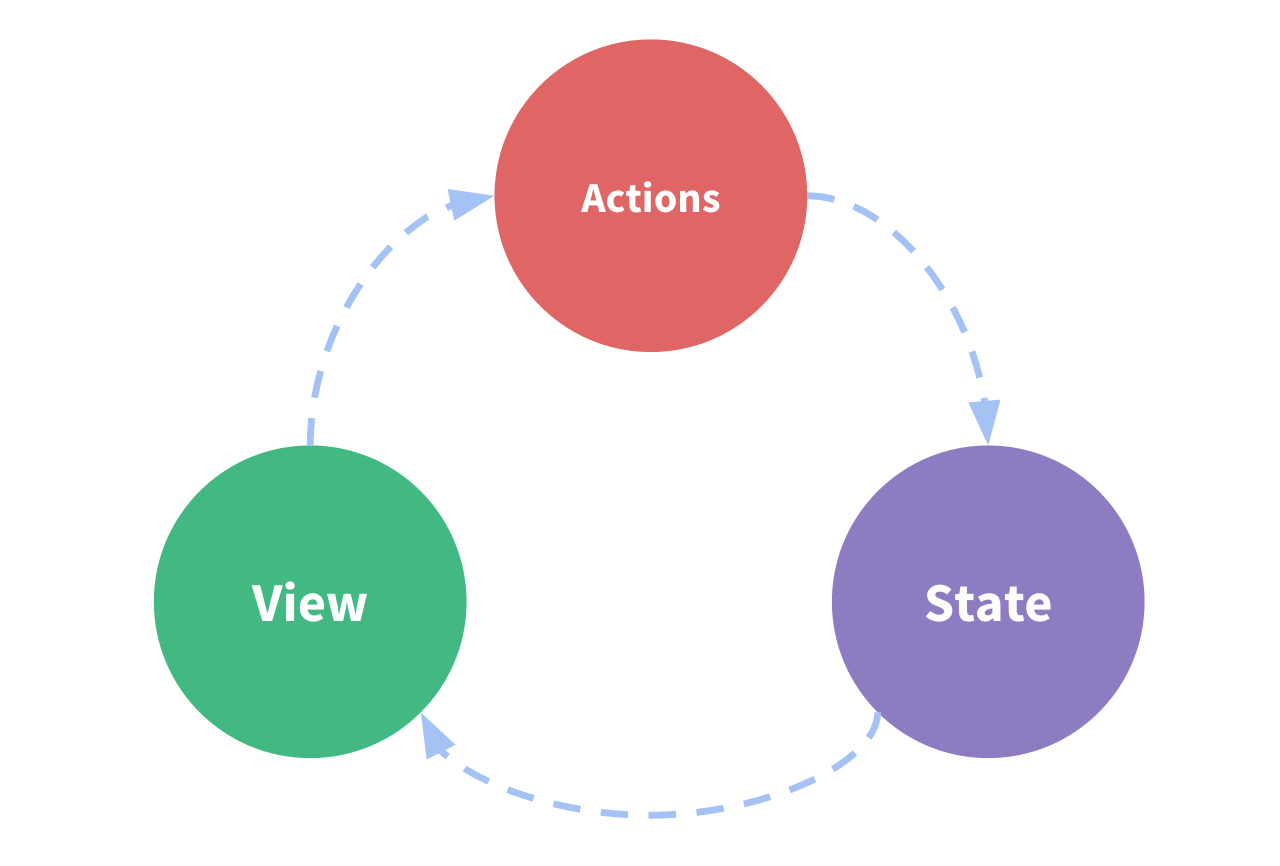
\includegraphics[width=4in,keepaspectratio]{flow-vuex.png}
		\caption{Vuex work flow}
		\label{label-vuex}
	\end{figure}
	\subsection{Swagger}
		\begin{wrapfigure}{L}{0.2\linewidth}
		\centering
		
\includegraphics[width=0.8in]{Swagger-logo.png}	
		
	\end{wrapfigure}
	\textbf{``Swagger''} tools were used to document the APIs of our application, which made it easier to test our APIs before using them. \textbf{``Swagger''} is a specification for documenting REST API. It specifies the format (URL, method, and representation) to describe REST web services. The methods, parameters, and models description are tightly integrated into the server code, thereby maintaining the synchronization in APIs and its documentation.\cite{swaggerArticle}
	\section{Used software}
	\subsection{Android studio}
	\begin{wrapfigure}{L}{0.2\linewidth}
		\centering
		
\includegraphics[width=0.8in]{aslogo.png}	
		
	\end{wrapfigure}
	We chose \textbf{``Android Studio''}; also developed by \textbf{``JETBRAINS''} for GOOGLE's operating system, as an IDE to develop our android application. Android Studio is fully featured \ac{ide} designed specifically for Android development. Automatically, it integrates the \ac{sdk} that enables developers to create applications for the Android platform\footnote{https://developer.android.com/studio/}.\par
	\clearpage
	\subsection{Visual studio code}
	\begin{wrapfigure}{L}{0.2\linewidth}
		\centering
		
\includegraphics[width=0.8in]{vsc-logo.png}	
		
	\end{wrapfigure}
	For the back-office code we decided on visual studio code as an \ac{ide}.\par 
	\textbf{``\ac{vsc}''} is a code editor redefined and optimized for building and debugging modern web and cloud applications.\par 
	Visual Studio Code combines the simplicity of a code editor with what developers need for their core edit-build-debug cycle. It provides comprehensive code editing, navigation, and understanding support along with lightweight debugging, a rich extensibility model, and lightweight integration with existing tools.
	\subsection{Laragon}
	\begin{wrapfigure}{L}{0.2\linewidth}
		\centering
		
\includegraphics[width=0.8in]{laragonlogo.png}	
		
	\end{wrapfigure}
	\textbf{``Laragon''} is a software that proposes to solve these problems by grouping all the tools you need for your development in a single installer.\par 
	The decision on using \textbf{``Laragon''} as a development server depend on various reasons, it is easy to use, it is  a modern, maintained and rich-featured local development environment.

	\subsection{Star UML}
	\begin{wrapfigure}{l}{0.1\linewidth}
		\centering
		
\includegraphics[width=0.6in]{staruml.png}
	\end{wrapfigure}
	We used \textbf{``Star UML''} to concept our different application's diagrams. Star UML is developed by \textbf{``MKLAB''}. It is an open source project to develop fast, flexible, and extensible UML conceptions' diagrams\footnote{staruml.io/}.\\
	\clearpage
	\subsection{TexStudio}
	\begin{wrapfigure}{l}{0.1\linewidth}
		\centering
		
\includegraphics[width=0.6in]{texstudio.png}
	\end{wrapfigure}
	We used \textbf{``TexStudio''}\footnote{https://www.texstudio.org/} as an IDE for creating our \textbf{``Latex''} report. As we used \textbf{``JABREF''}\footnote{http://www.jabref.org/} to include the bibliography in our document. \LaTeX~is a high-quality typesetting system; it includes features designed for the production of technical and scientific documentation as it is the de facto standard for the communication and publication of scientific documents.\cite{latexBook}
	
	\subsection{SourceTree}
	\begin{wrapfigure}{l}{0.1\linewidth}
		\centering
		
\includegraphics[width=0.6in]{sourcetreelogo.png}
	\end{wrapfigure}
	A Git GUI that offers a visual representation of your repositories.\textbf{``Sourcetree''}  is a free Git client.\par 
	It simplifies how we interact with the Git repositories which offers an easy and fast way for us to save our progress in the code.
	\section*{Conclusion}
	\addcontentsline{toc}{section}{Conclusion}
	We have detailed the general architecture detailing the used technologies and framework to make this work possible.
	In the next chapter we will pass part 1 of the SCRUM methodology, the release 1 which will detail and present its user story.
	\chapter{Release 1}
	\section*{Introduction}
	\addcontentsline{toc}{section}{Introduction}
	In the previous chapter, we discussed in detail the architecture of the \textbf{``CakeitUp''} application followed by all the used technologies to make this work.\par 
	This chapter is concerned with the presentation of the release 1, where we will detail the different stages of creation of this system.
	\section{Backlog}

	\begin{table}[H]
		\begin{center}
			\captionsetup[table]{skip=10pt}
			\caption{Backlog: Release 1}
			\setlength\doublerulesep{0.5pt}
			\begin{tabular}{|  p{3cm}|  p{1cm}| p{4cm}|  p{1cm}| p{6cm}|}
				\hline 
				\rowcolor{LightCyan}
				 \textbf{Sprint} & \textbf{ID \ac{us}} & \textbf{User story} & \textbf{ID task} & \textbf{Task} 
				\\ \hline
				\multirow{5}{3cm}{\textbf{Sprint 1} \textbf{Authentication} }
				&                       
				1.1  &  
				\multirow{2}{4cm}{As an unauthorized User i want to create a new account.}
				              
				&				                      
				1.1.A &                        
				Make the diagrams needed for this \ac{us} (use case diagram, class diagram, sequence diagram).
				\\ 
				\cline{4-5}    
				&                   
			      &                                 
				&                        
				1.1.B &                        
				Develop the inscription model.
				\\ 
				\cline{4-5}    
				&                   
				&                                 
				&                        
				1.1.C &                        
				Test the inscription model.
			
				
				
			\end{tabular}
			
		\end{center}
		
	\end{table}
	\begin{table}[H]
	\begin{center}
		\setlength\doublerulesep{0.5pt}
		\begin{tabular}{|  p{3cm}|  p{1cm}| p{4cm}|  p{1cm}| p{6cm}|}
			 \cline{2-5}  
			
			&                       
			1.2  &  
			\multirow{2}{4cm}{As an unauthorized User i want to login.}
			
			&				                      
			1.2.A &                        
				Make the diagrams needed for this \ac{us}.
			\\ 
			\cline{4-5}    
			&                   
			&                                 
			&                        
			1.2.B &                        
			Develop the login model.
				\\ 
			\cline{4-5}    
			&                   
			&                                 
			&                        
			1.2.C &                        
			Test the login model.
			\\
			\cline{2-5}  
			
			&                       
			1.3  &  
			\multirow{2}{4cm}{As an 
				authorized User i want to logout.}
			
			&				                      
			1.3.A &                        
			Make the diagrams needed for this \ac{us}.
			\\ 
			\cline{4-5}    
			&                   
			&                                 
			&                        
			1.3.B &                        
			Develop the logout model.
			\\ 
			\cline{4-5}    
			&                   
			&                                 
			&                        
			1.3.C &                        
			Test the logout model.
			\\
			\cline{2-5}  
			
			&                       
			1.4  &  
			\multirow{2}{4cm}{As an 
				unauthorized User i want to reset my password.}
			
			&				                      
			1.4.A &                        
			Make the diagrams needed for this \ac{us}.
			\\ 
			\cline{4-5}    
			&                   
			&                                 
			&                        
			1.4.B &                        
			Develop the reset password model.
			\\ 
			\cline{4-5}    
			&                   
			&                                 
			&                        
			1.4.C &                        
			Test the reset password model.
			\\ \hline
			\multirow{5}{3cm}{\textbf{Sprint 2} \textbf{Manage account} }
			&                       
			2.1  &  
			\multirow{2}{4cm}{As a authorizer user i want to edit my account.}
			
			&				                      
			2.1.A &                        
			Make the diagrams needed for this \ac{us} (use case diagram, class diagram, sequence diagram).
			\\ 
			\cline{4-5}    
			&                   
			&                                 
			&                        
			2.1.B &                        
			Develop the edit pastry model.
			\\ 
			\cline{4-5}    
			&                   
			&                                 
			&                        
			2.1.C &                        
			Test the edit pastry model.
			\\ \hline
			\multirow{5}{3cm}{\textbf{Sprint 3} \textbf{Manage pastries} }
			&                       
			3.1  &  
			\multirow{2}{4cm}{As a pastry owner i want to edit my own pastry.}
			
			&				                      
			3.1.A &                        
			Make the diagrams needed for this \ac{us} (use case diagram, class diagram, sequence diagram).
			\\ 
			\cline{4-5}    
			&                   
			&                                 
			&                        
			3.1.B &                        
			Develop the edit pastry model.
			\\ 
			\cline{4-5}    
			&                   
			&                                 
			&                        
			3.1.C &                        
			Test the edit pastry model.
			\\
			\cline{2-5}  
			
			&                       
			3.2  &  
			\multirow{2}{4cm}{As an administrator i want to block pastries.}
			
			&				                      
			3.2.A &                        
			Make the diagrams needed for this \ac{us}.
			\\ 
			\cline{4-5}    
			&                   
			&                                 
			&                        
			3.2.B &                        
			Develop the block pastry model.
			\\ 
			\cline{4-5}    
			&                   
			&                                 
			&                        
			3.2.C &                        
			Test the block pastry model.
			\\
			\cline{2-5}  
			
			&                       
			3.3  &  
			\multirow{2}{4cm}{As an administrator i want to view list of pastries.}
			
			&				                      
			3.3.A &                        
			Make the diagrams needed for this \ac{us}.
			\\ 
			\cline{4-5}    
			&                   
			&                                 
			&                        
			3.3.B &                        
			Develop the list of pastries model.
			\\ 
			\cline{4-5}    
			&                   
			&                                 
			&                        
			3.3.C &                        
			Test the list of pastries model.
			
			
			
			
			
			
			
		\end{tabular}
		
	\end{center}
	
\end{table}
	\begin{table}[H]
		\begin{center}
			\setlength\doublerulesep{0.5pt}
			\begin{tabular}{|  p{3cm}|  p{1cm}| p{4cm}|  p{1cm}| p{6cm}|}
			
				\cline{2-5}  
				
				&                       
				3.4  &  
				\multirow{2}{4cm}{As an administrator i want to activate or dis-activate a pastry.}
				
				&				                      
				3.4.A &                        
				Make the diagrams needed for this \ac{us}.
				\\ 
				\cline{4-5}    
				&                   
				&                                 
				&                        
				3.4.B &                        
				Develop the activation/dis-activation pastry model.
				\\
				\cline{4-5}    
				&                   
				&                                 
				&                        
				3.4.C &                        
				Test the activation/dis-activation pastry model.
				\\
				\cline{2-5}  
				
				&                       
				3.5  &  
				\multirow{2}{4cm}{As a client i want to view and search list of activated pastries.}
				
				&				                      
				3.5.A &                        
				Make the diagrams needed for this \ac{us}.
				\\ 
				\cline{4-5}    
				&                   
				&                                 
				&                        
				3.5.B &                        
				Develop the list of pastries for the client.
				\\ 
				\cline{4-5}    
				&                   
				&                                 
				&                        
				3.5.C & 
				Test the list of pastries.                       
				\\
				\cline{2-5}  
				
				&                       
				3.6  &  
				\multirow{2}{4cm}{As a pastry owner i want dis-activate my own pastry if it is activated.}
				
				&				                      
				3.6.A &                        
				Make the diagrams needed for this \ac{us}.
				\\ 
				\cline{4-5}    
				&                   
				&                                 
				&                        
				3.6.B &                        
				Develop the pastry dis-activation model.
				\\ 
				\cline{4-5}    
				&                   
				&                                 
				&                        
				3.6.C &                        
				Test the pastry dis-activation model.
			
				\\
				 \hline
				\multirow{5}{3cm}{\textbf{Sprint 4} \textbf{Manage products} }
				&                       
				4.1  &  
				\multirow{2}{4cm}{As a pastry owner i want to add a product.}
				
				&				                      
				4.1.A &                        
				Make the diagrams needed for this \ac{us} (use case diagram, class diagram, sequence diagram).
				\\ 
				\cline{4-5}    
				&                   
				&                                 
				&                        
				4.1.B &                        
				Develop the add product model.
				\\ 
				\cline{4-5}    
				&                   
				&                                 
				&                        
				4.1.C &                        
				Test the add product model.
				\\
				\cline{2-5}  
				
				&                       
				4.2  &  
				\multirow{2}{4cm}{As a pastry owner i want to edit a product.}
				
				&				                      
				4.2.A &                        
				Make the diagrams needed for this \ac{us}.
				\\ 
				\cline{4-5}    
				&                   
				&                                 
				&                        
				4.2.B &                        
				Develop the edit product model.
				\\ 
				\cline{4-5}    
				&                   
				&                                 
				&                        
				4.2.C &                        
				Test the edit product model.
				\\
				\cline{2-5}  
				
				&                       
				4.3  &  
				\multirow{2}{4cm}{As a pastry owner i want to view list of products.}
				
				&				                      
				4.3.A &                        
				Make the diagrams needed for this \ac{us}.
				\\ 
				\cline{4-5}    
				&                   
				&                                 
				&                        
				4.3.B &                        
				Develop the list of products model.
				\\ 
				\cline{4-5}    
				&                   
				&                                 
				&                        
				4.3.C &                        
				Test the list of products model.
			
				
				
				
			\end{tabular}
			
		\end{center}
		
	\end{table}
	\begin{table}[H]
	\begin{center}
		\setlength\doublerulesep{0.5pt}
		\begin{tabular}{|  p{3cm}|  p{1cm}| p{4cm}|  p{1cm}| p{6cm}|}
			
		
		\cline{2-5}  
		
		&                       
		4.4  &  
		\multirow{2}{4cm}{As a pastry owner i want to archive a product.}
		
		&				                      
		4.4.A &                        
		Make the diagrams needed for this \ac{us}.
		\\ 
		\cline{4-5}    
		&                   
		&                                 
		&                        
		4.4.B &                        
		Develop the archive a product model.
		\\ 
		\cline{4-5}    
		&                   
		&                                 
		&                        
		4.4.C &                        
		Test the archive a product model.
		
		\\
		\hline
			
		\end{tabular}
		
	\end{center}
	
\end{table}
\section{Use case}
\subsection{Use case diagram}
We will be deviding the use case of the release 1 depending on each sprint, starting by the first sprint \textbf{``Authentication''} presented in Figure \ref{auth-diag}.
\begin{figure}[H]
	\centering
	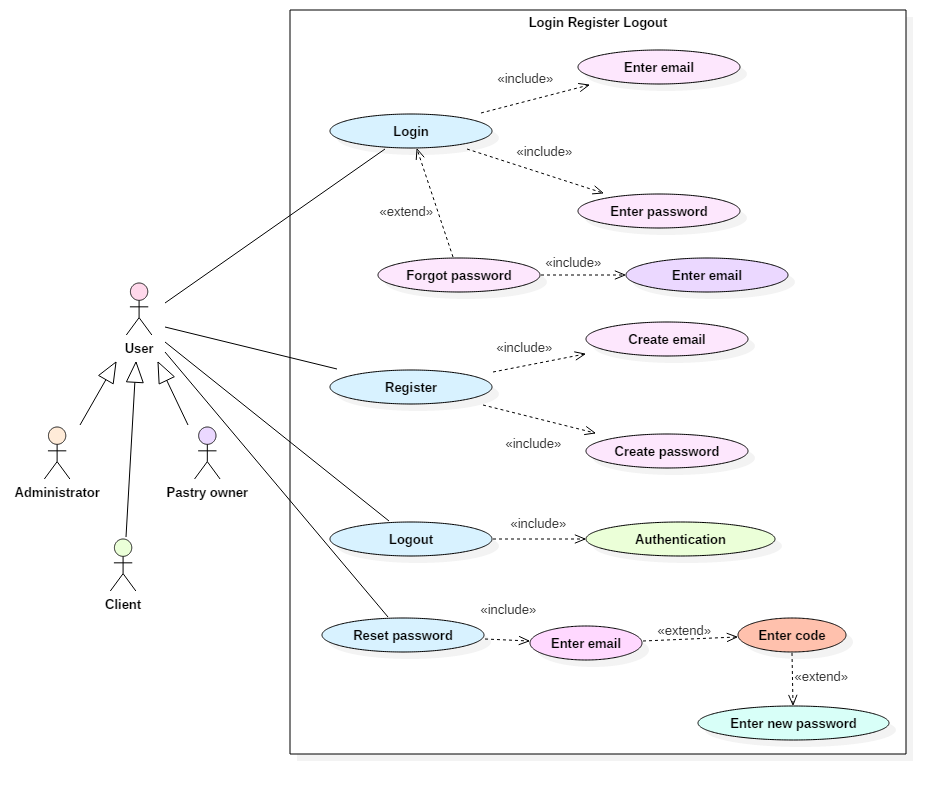
\includegraphics[width=6in,keepaspectratio]{auth.png}
	\caption{Use case Authentication}
	\label{auth-diag}
\end{figure}
\clearpage
In Figure \ref{edit-account} we introduce the different use case of the sprint 2 \textbf{``Manage account''}.
\begin{figure}[H]
	\vspace*{3cm}
	\centering
	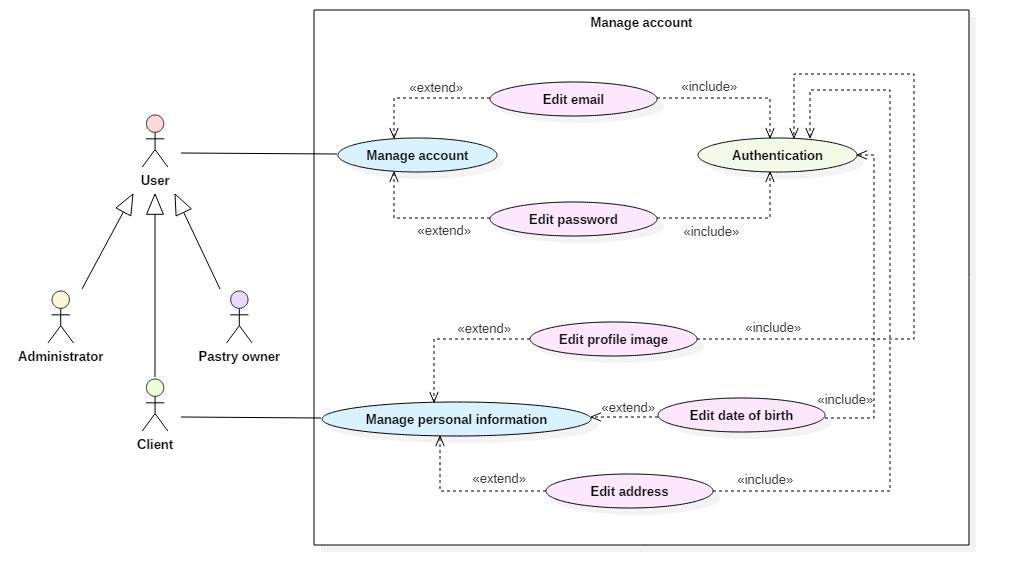
\includegraphics[width=7.2in,keepaspectratio]{manageAccount.png}
	\caption{Use case edit account}
	\label{edit-account}
\end{figure}
We will be giving an idea about the sprint 3 \textbf{``Manage pastries''} via Figure \ref{edit-pastry}.
\begin{figure}[H]
	\centering
	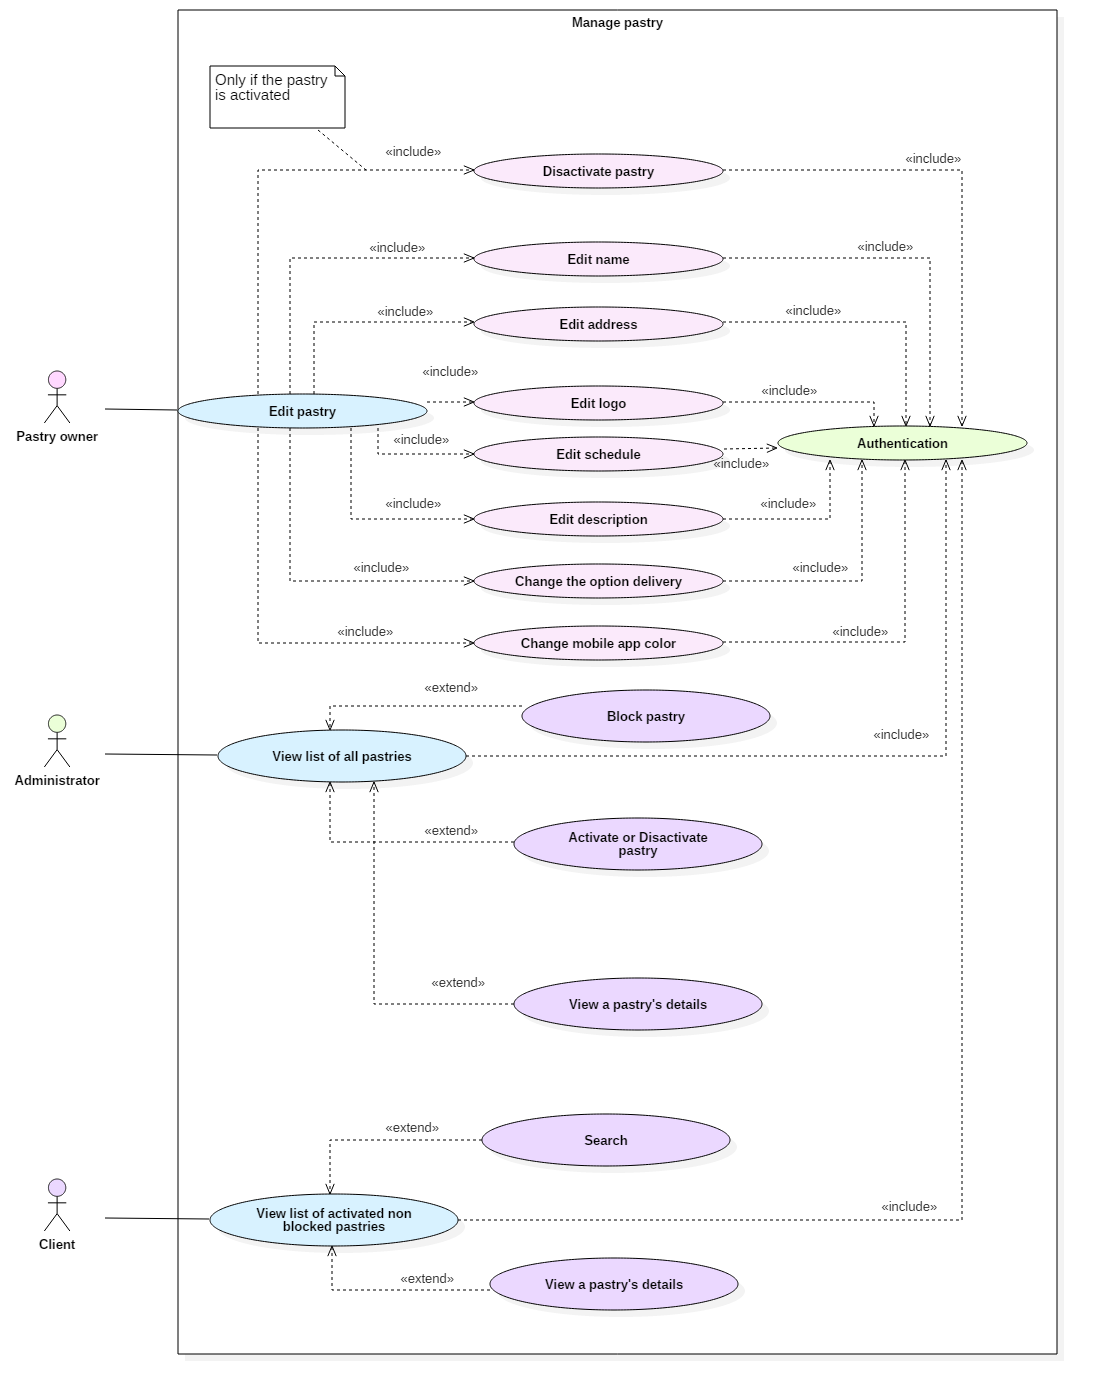
\includegraphics[width=7.2in,keepaspectratio]{editPastry.png}
	\caption{Use case manage pastries}
	\label{edit-pastry}
\end{figure}
Figure \ref{edit-product} is a graphic presentation of sprint 4 \textbf{``Manage products''}.
\begin{figure}[H]
	\vspace*{2cm}
	\centering
	\includegraphics[width=7.2in,keepaspectratio]{ManageProducts.png}
	\caption{Use case manage products}
	\label{edit-product}
\end{figure}
\subsection{Use case description}
\subsubsection*{Use case "Authentication" description}
\begin{table}[H]
	\begin{center}
		\captionsetup[table]{skip=10pt}
		\caption{Use case "Authentication" description}
		\setlength\doublerulesep{0.5pt}
\begin{tabular}{|  p{5cm}|  p{9cm}|}
	\rowcolor{LightCyan}
	
	\hline
	\multicolumn{2}{c}{Use case "Authentication"}\\
	\hline
	
	\textbf{Actors} &                        
	User 
	\\ \hline
	
	\textbf{Precondition} &                        
	Have or will create an account 
\\ \hline
	\textbf{Postcondition} &                        
	The user have ,will create an account or is already logged in 
	\\ \hline
	
	\textbf{Main scenario} &                        
	\begin{itemize}
		\item The user does not have an account
		\begin{itemize}
			\item The system will require the used to fill in the email, password and confirm password,
			\item The user fill in the form,
			\item The system verify the information,
			\item the system shows the home of the application whether it is the web or mobile.
		\end{itemize}
		\item The user have an account and is not logged in
		\begin{itemize}
			\item The system will require the used to fill in the email and password,
			\item The user fill in the form,
			\item The system verify the information,
			\item the system shows the home of the application whether it is the web or mobile.
		\end{itemize}

		
		
	\end{itemize} 

	
	
\end{tabular}
\end{center}

\end{table}
\begin{table}[H]
	\begin{center}

		\setlength\doublerulesep{0.5pt}
\begin{tabular}{|  p{5cm}|  p{9cm}|}
	
	 &                        
	\begin{itemize}
	
		\item The user have an account and is logged in
		\begin{itemize}
			\item The system will ask for logout confirmation,
			\item The user will confirm,
			\item The system will log out the user and show the login page.
		\end{itemize}
		
		
	\end{itemize} 
	\\ \hline
	
	\textbf{Alternative scenario} &                        
	In case of an error the system will show an error message.
	\\ \hline
	
	

\end{tabular}

\end{center}

\end{table}
\subsubsection*{Use case "Manage account" description}
\begin{table}[H]
	\begin{center}
		\captionsetup[table]{skip=10pt}
		\caption{Use case "Manage account" description}
		\setlength\doublerulesep{0.5pt}
\begin{tabular}{|  p{5cm}|  p{9cm}|}
	\rowcolor{LightCyan}
	
	\hline
	\multicolumn{2}{c}{Use case "Manage account"}\\
	\hline
	
	\textbf{Actors} &                        
	User 
	\\ \hline
	
	\textbf{Precondition} &                        
	The user is authenticated
	\\ \hline
	\textbf{Postcondition} &                        
	account edited
	\\ \hline
	
	\textbf{Main scenario} &                   
	\begin{itemize}
		\item The user access his account ,
		\item The user his account,
		\item The system will save the changes.
	\end{itemize}
	
	 
	\\ \hline
	
	\textbf{Alternative scenario} &                        
	In case of an error the system will show an error message.
	\\ \hline
	
	
\end{tabular}

\end{center}

\end{table}
\subsubsection*{Use case "Manage pastries" description}
\begin{table}[H]
	\begin{center}
		\captionsetup[table]{skip=10pt}
		\caption{Use case "Manage pastries" description}
		\setlength\doublerulesep{0.5pt}
		\begin{tabular}{|  p{5cm}|  p{9cm}|}
			\rowcolor{LightCyan}
			
			\hline
			\multicolumn{2}{c}{Use case "Manage pastries"}\\
			\hline
			
			\textbf{Actors} &                        
			User 
			\\ \hline
			
			\textbf{Precondition} &                        
			Pastry exists ,user connected and authorized
			\\ \hline
			\textbf{Postcondition} &                        
			Pastry edited
			\\ \hline
			
			\textbf{Main scenario} &                        
			
				\begin{itemize}
					\item The user access the specific pastry to edit, dis-activate, activate or block,
					\item The user edit the pastry,
					\item The system will save the changes.
				\end{itemize}
				
			\\ \hline
			
			\textbf{Alternative scenario} &                        
			In case of an error the system will show an error message.
			\\ \hline
			
			
		\end{tabular}
		
	\end{center}
	
\end{table}
\subsubsection*{Use case "Manage products" description}
\begin{table}[H]
	\begin{center}
		\captionsetup[table]{skip=10pt}
		\caption{Use case "Manage products" description}
		\setlength\doublerulesep{0.5pt}
		\begin{tabular}{|  p{5cm}|  p{9cm}|}
			\rowcolor{LightCyan}
			
			\hline
			\multicolumn{2}{c}{Use case "Manage products"}\\
			\hline
			
			\textbf{Actors} &                        
			User 
			\\ \hline
			
			\textbf{Precondition} &                        
			The user is authenticated and authorized
			\\ \hline
			\textbf{Postcondition} &                        
			Product added or edited
			\\ \hline
			
			\textbf{Main scenario} &                   
			\begin{itemize}
				\item The user access the list of products,
				\item The user make changes,
				\item The system will save the changes.
			\end{itemize}
			
			
			\\ \hline
			
			\textbf{Alternative scenario} &                        
			In case of an error the system will show an error message.
			\\ \hline
			
			
		\end{tabular}
		
	\end{center}
	
\end{table}
\section{Sequence diagram}
We will be presenting multiple sequence diagrams for some of the sprints we have in this release.\par
\subsubsection*{Sequence diagram "Authentication"}
Starting by the first sprint \textbf{Authentication} showing in Figure \ref{auth-sequence}. The use whether it is an administrator, pastry owner or even a client if he is not logged in he has two option either create an account or login in he already have an account, To create an account all he has to do is to enter the required information (email, password and password confirmation) if all is good the controller will ask the database for the information needed to create the session such as a token and also send a notification and a mail to the administrator and will redirect the use to the home interface, else if the is any kind of an error the system will show an error message describing the error and ask the user to try again.\par 
In case the user already have an account he can login by giving the email and password on condition they are valid and match a record on the database, if not the user will receive an error message.\par 
Last but not least, the user is logged in and wants to end his visit, he can simply logout.
\begin{figure}[H]
	\centering
	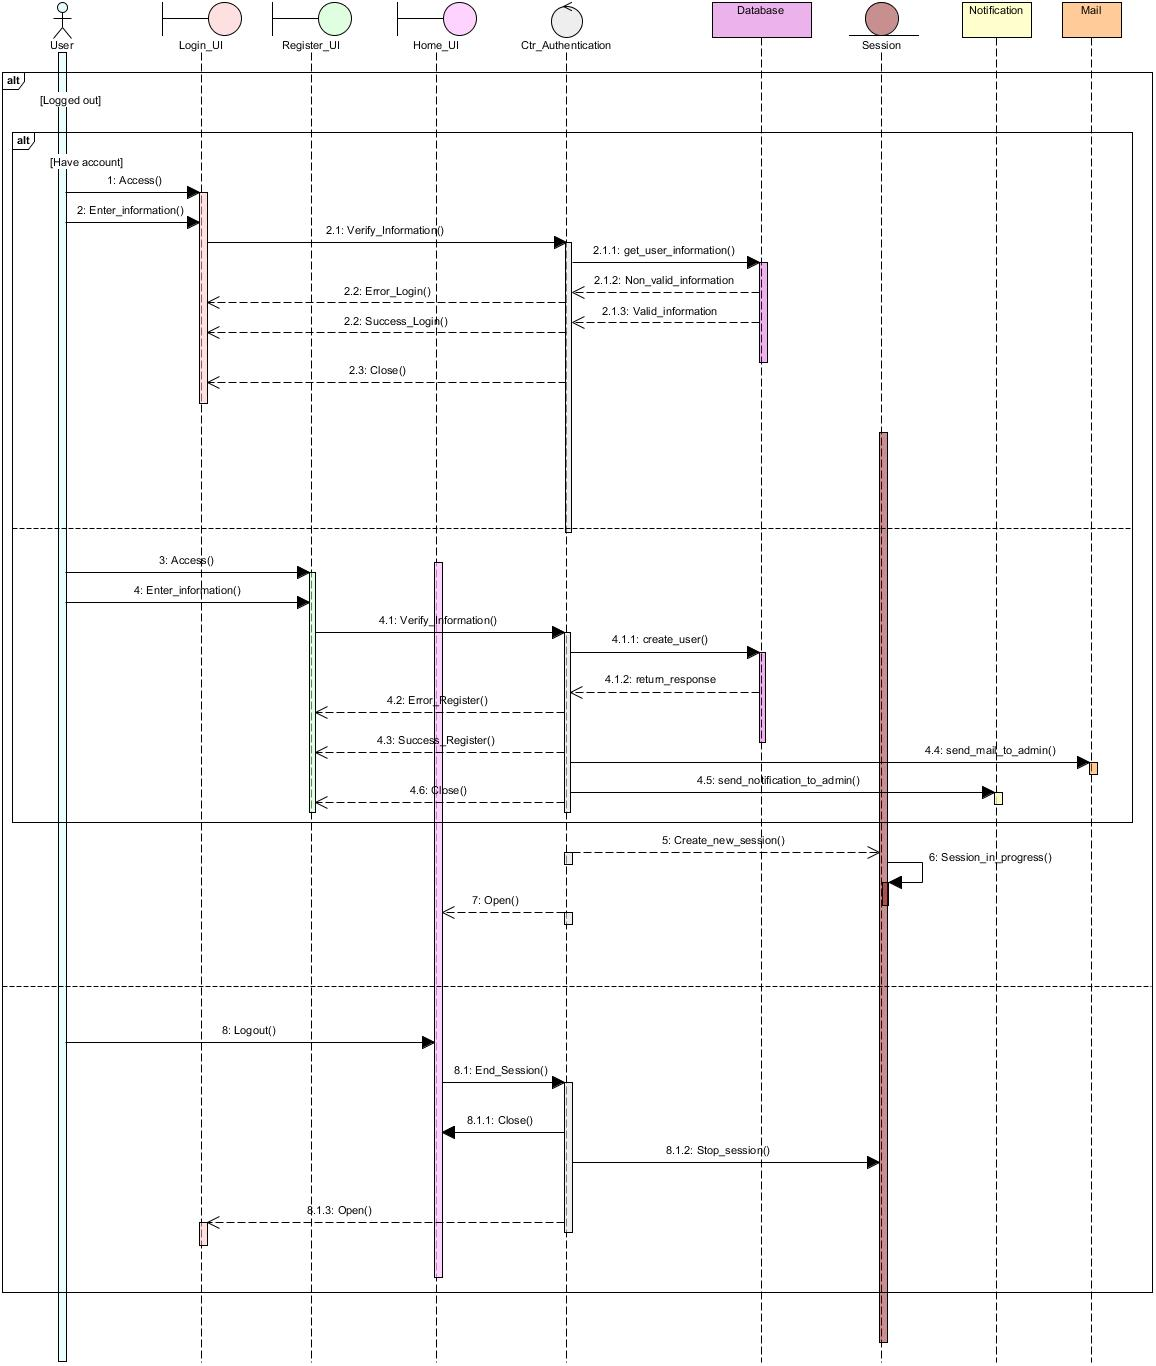
\includegraphics[width=7in,keepaspectratio]{authSequence.jpg}
	\caption{Authentication sequence diagram}
	\label{auth-sequence}
\end{figure}

\subsubsection*{Sequence diagram "Manage product"}
Figure \ref{product-sequence} represent the sequence diagram for the last sprint of this release \textbf{Manage product}.\par 
As we descried before this sprint has four U.S:
\begin{itemize}
	\item Add product: \par 
	To add a product the pastry owner should access the add product interface and fill in the required data for the it (name; image, description, price, ingredients ...), the next step is to confirm his addition, the controller will receive the data and verify them, in case all is good, the product is saved to the database and the controller will wait for a response from it, after that the user will be redirected the list of products including the new product that was just added.
	\item Edit product: \par 
	Editing a product will take basically the same steps as adding one, first of all the user will access the edit interface of a specific product, he will make the changes that he wants to make and confirm them. The controller will receive those changes and verify every one of them, if the verification is a success, the controller will update the requested product and redirect the user to the show product interface.
	\item View list of products: \par 
	As for viewing the list of products, the pastry owner just needs to navigate to the list of products interface, and the controller will request the list from the database and send it back to the view.
	\item Archive a product: \par 
	In order to archive a product the user needs to access the list of products list first and select the archive button, the controller will make a request to the database to add this product to the archived list then it will show a success message or an error message depending on the database response. 
\end{itemize}
\begin{figure}[H]
	\centering
	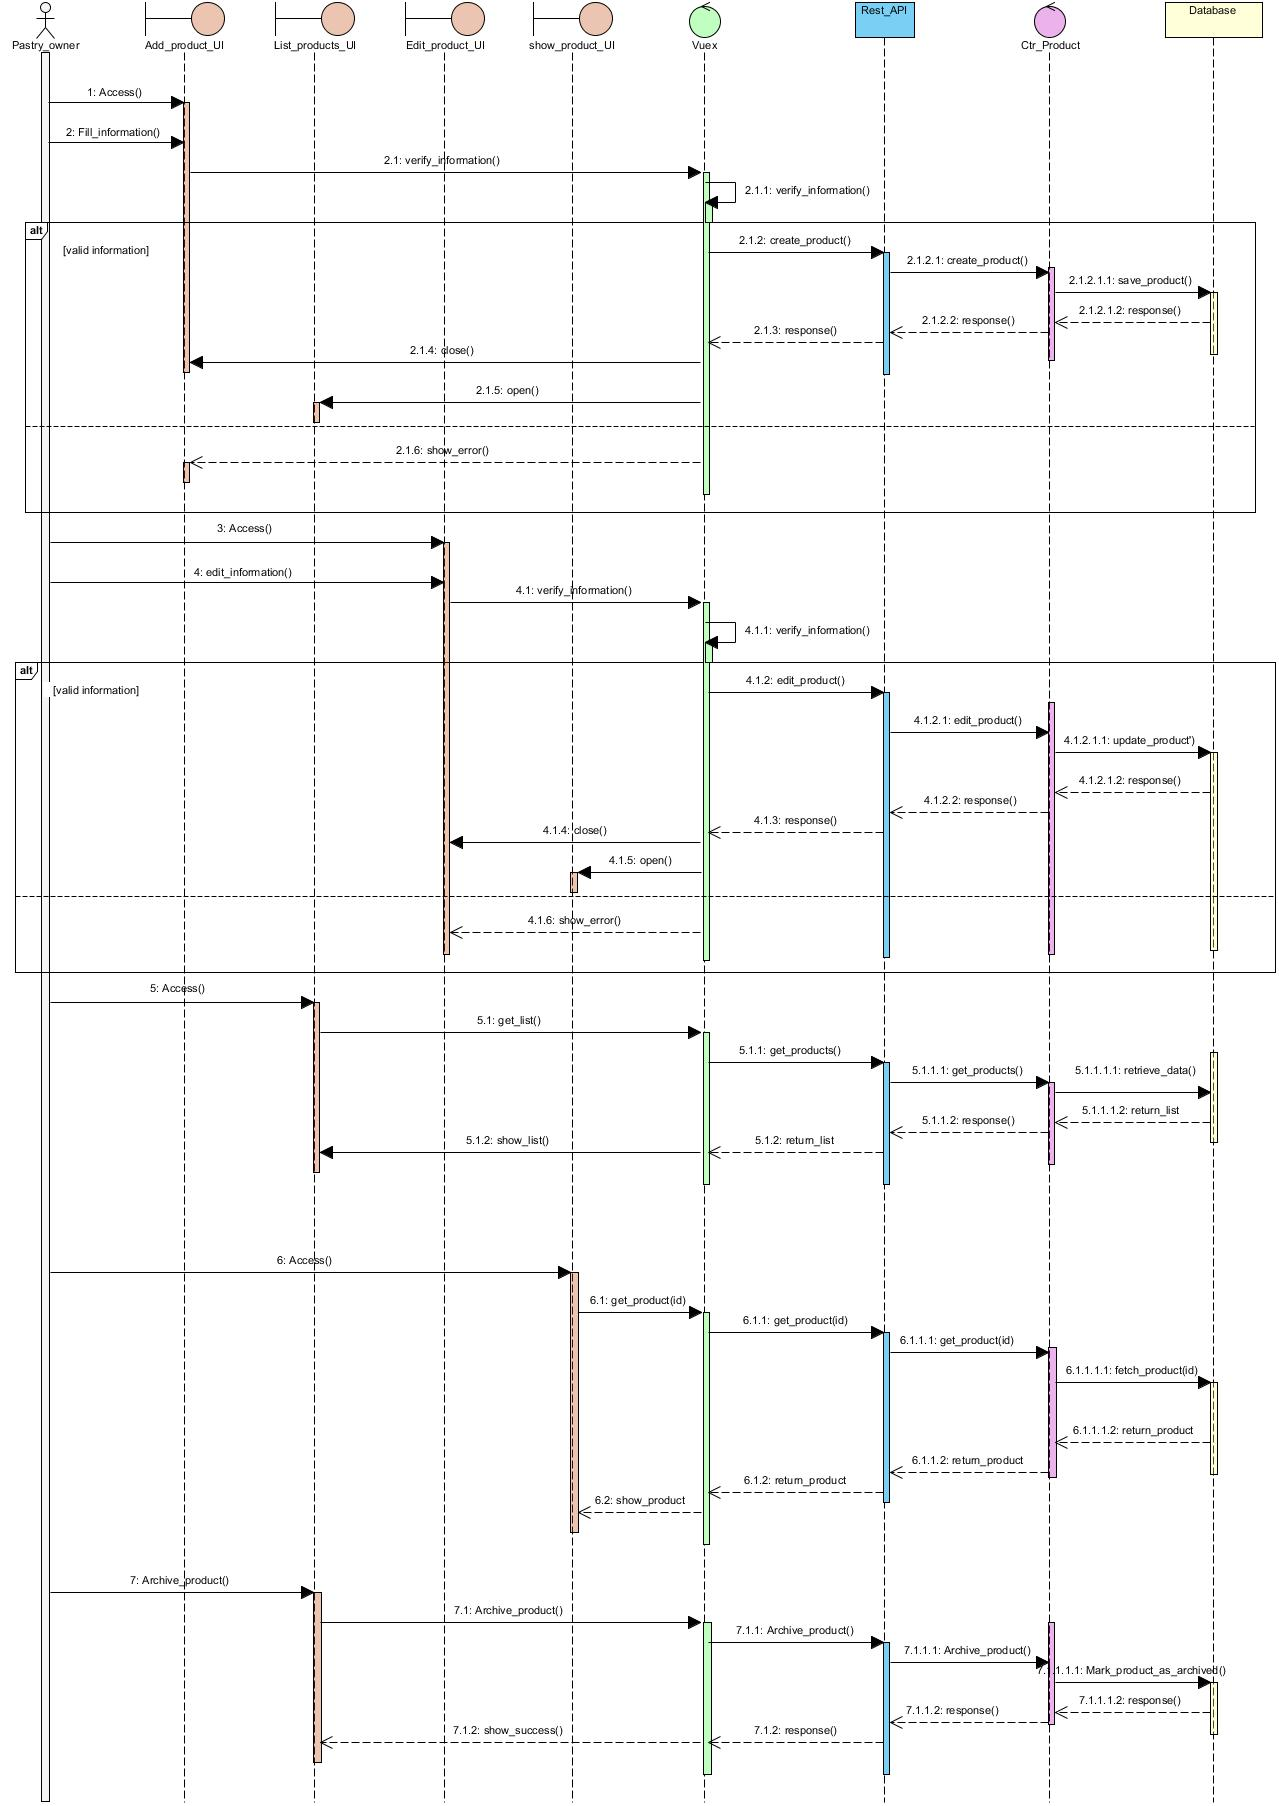
\includegraphics[width=6.7in,keepaspectratio]{manageproduct.jpg}
	\caption{Manage product sequence diagram}
	\label{product-sequence}
\end{figure}
\section{Implementation}
	We will be presenting the different interface of our mobile and web application for this release.\par
\subsection{Web}
\subsubsection*{Sprint "Authentication"}
Starting by the authentication (login, register, reset password, logout), Figure \ref{register-interface} shows the interface for the register task for the web application where the use have to fill in the form in order to create a pastry owner account, all the entered data has to be valid, in case of an error the system will show the user where is the mistake.
\begin{figure}[H]
	\vspace*{2cm}
	\centering
	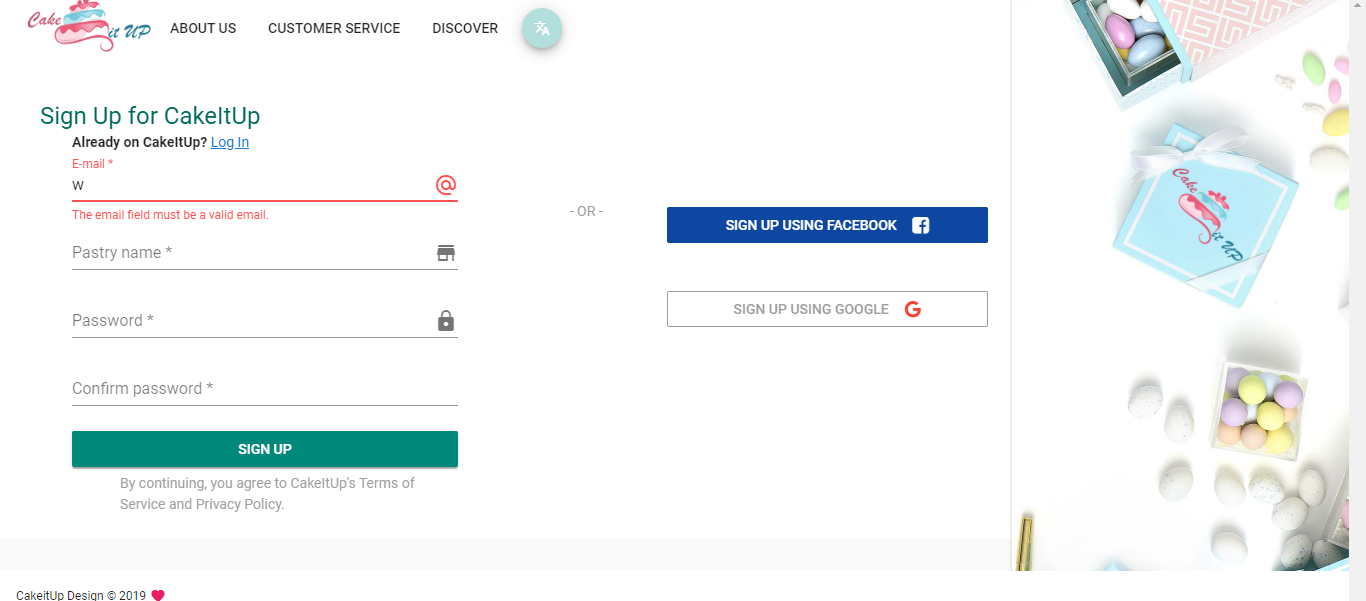
\includegraphics[width=7in,keepaspectratio]{register.png}
	\caption{Register interface web}
	\label{register-interface}
\end{figure}
\clearpage
As shown in Figure \ref{login-interface}, the interface of login is simple and elegant, the user will fill in the data and login if no error has been displayed.
\begin{figure}[H]
	\centering
	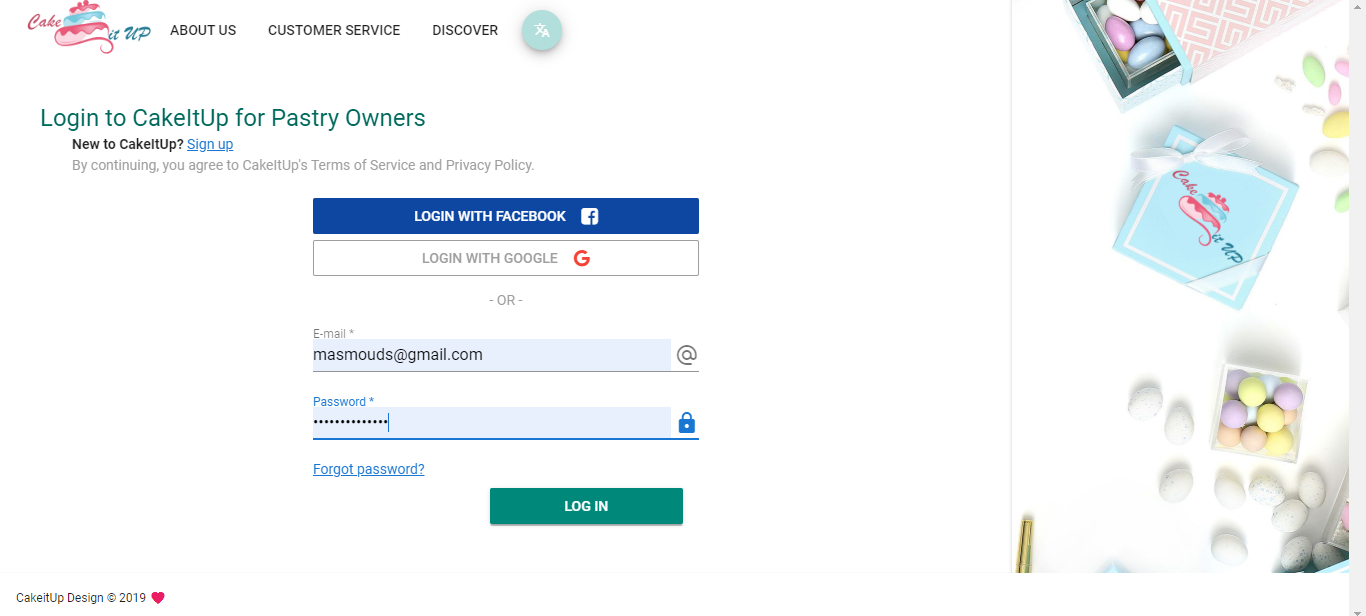
\includegraphics[width=6.5in,keepaspectratio]{login.png}
	\caption{Login interface web}
	\label{login-interface}
\end{figure}
In case the used forgot his password, he can rest it by entering his email as shown in Figure \ref{resetpassword-interface}, a mail bill be send to him with the code needed to reset the password, once he entered the code, it will be verified if it is the right one the system will show the next step which is resetting the password.
\begin{figure}[H]
	\centering
	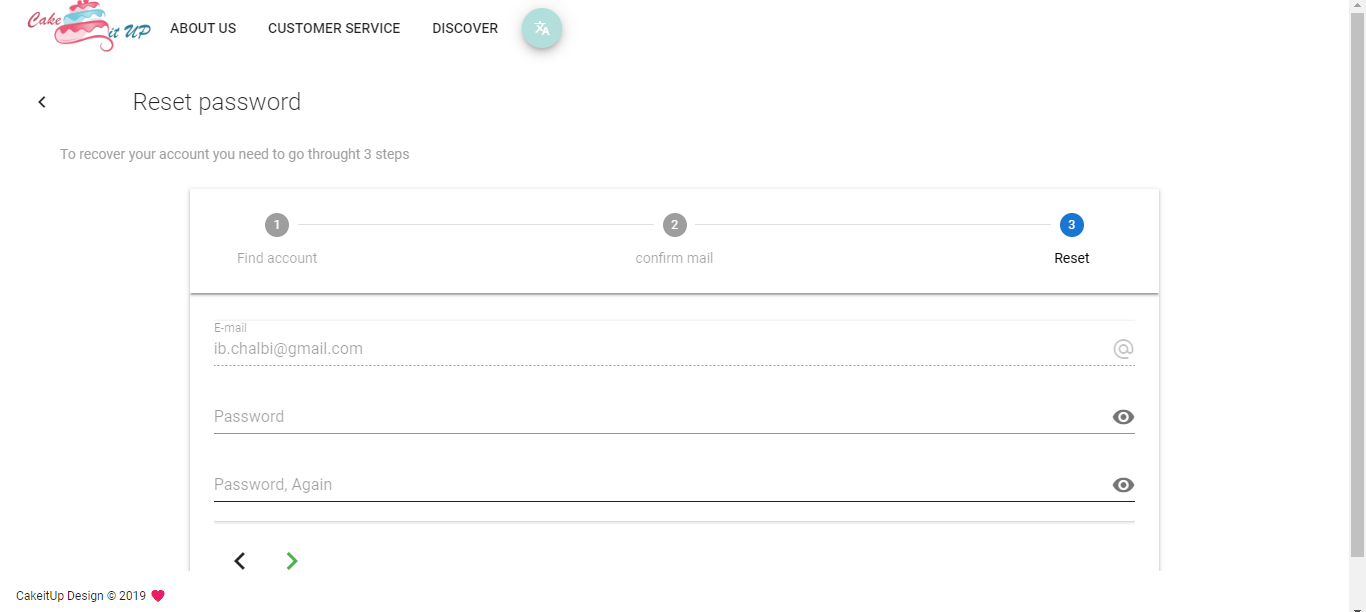
\includegraphics[width=6.5in,keepaspectratio]{reset-password.png}
	\caption{Reset password interface web}
	\label{resetpassword-interface}
\end{figure}
\clearpage
Once the use has been logged in he has the ability to logout by a simple click as presented in Figure \ref{logout-interface}.
\begin{figure}[H]
	\centering
	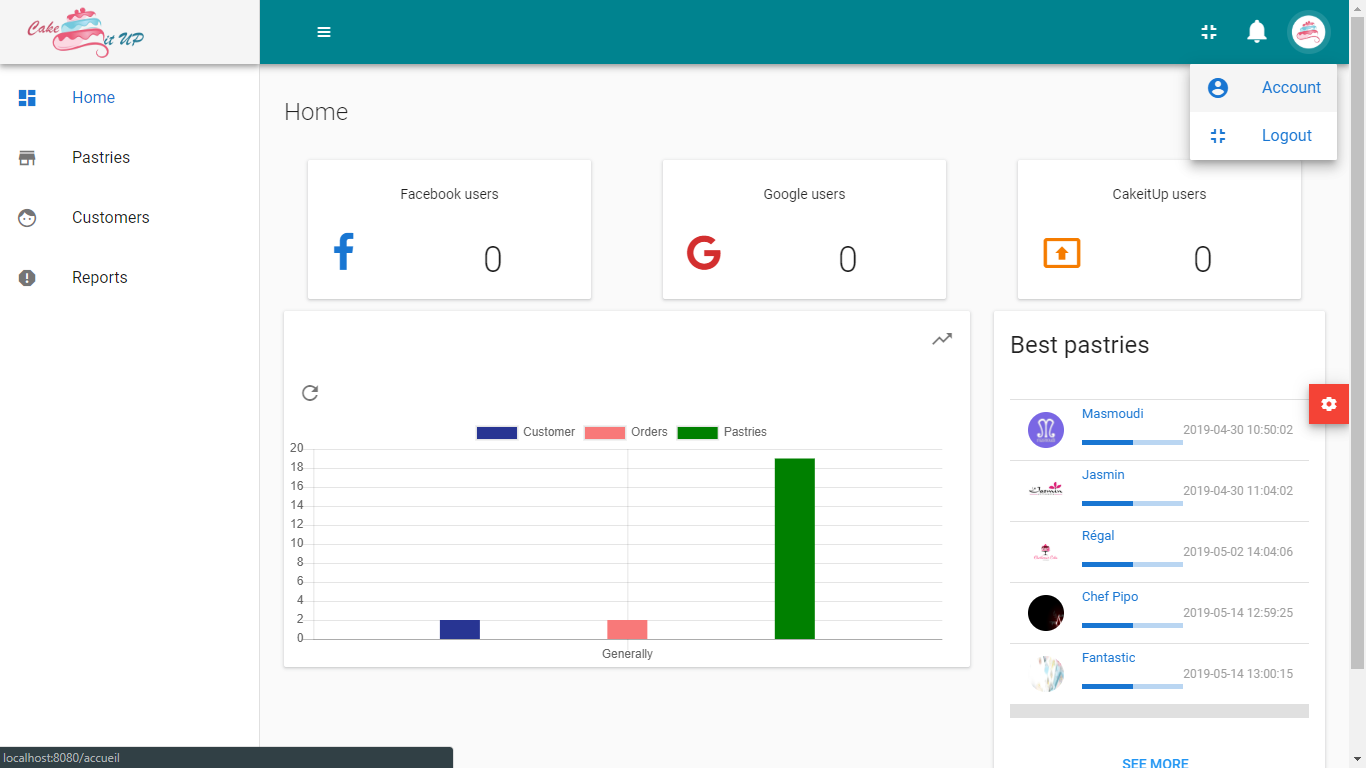
\includegraphics[width=5.5in,keepaspectratio]{logout.png}
	\caption{Logout interface web}
	\label{logout-interface}
\end{figure}
\subsubsection*{Sprint "Manage account"}
Both the web users (Administrator and pastry owner) have the permission to edit their account, they can change the email and their password as well.
\begin{figure}[H]
	\centering
	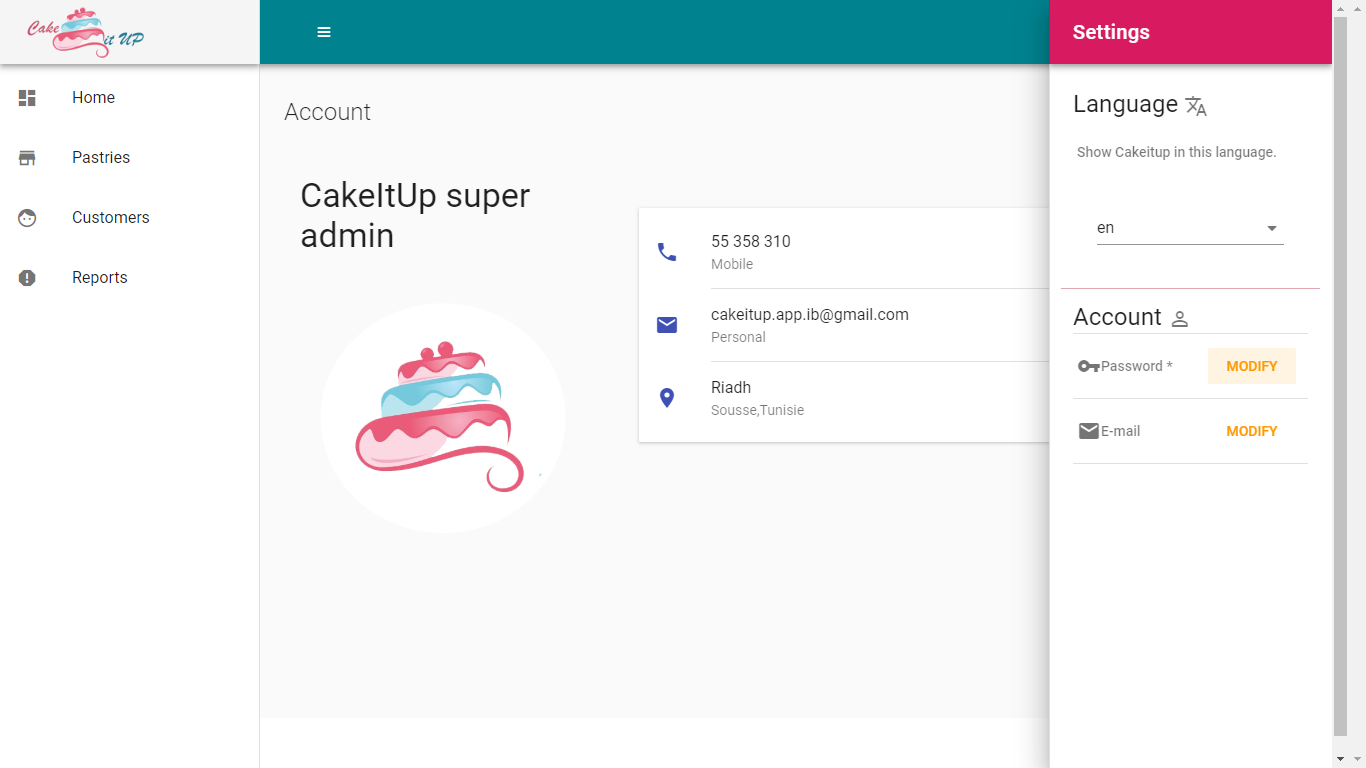
\includegraphics[width=6in,keepaspectratio]{manageaccountAdmin.png}
	\caption{Edit account interface web}
	\label{editaccountadmin-interface}
\end{figure} 
\subsubsection*{Sprint "Manage pastries"}
The administrator can view the list of all pastries where he can access to just one of them, block them, activate or dis-activate them as we can see in Figure \ref{pastrylist-interface}.
\begin{figure}[H]
	\centering
	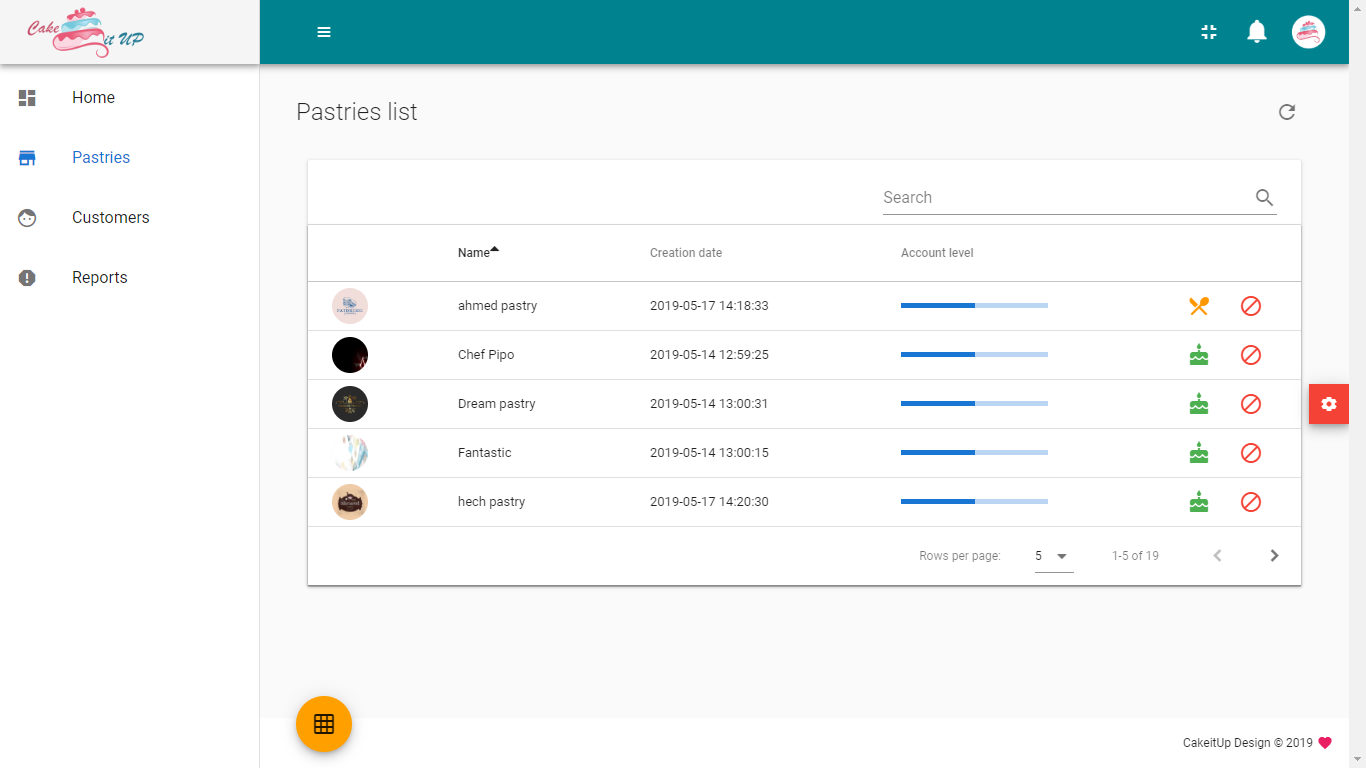
\includegraphics[width=5.6in,keepaspectratio]{pastry-list.png}
	\caption{List of pastries interface web}
	\label{pastrylist-interface}
\end{figure} 

We have already gave a detailed description of the task edit pastry, only the pastry owner can edit his own pastry, as shown in Figure \ref{editpastry-interface} the user can make a lot of changes depending on his choice.
\begin{figure}[H]
	\centering
	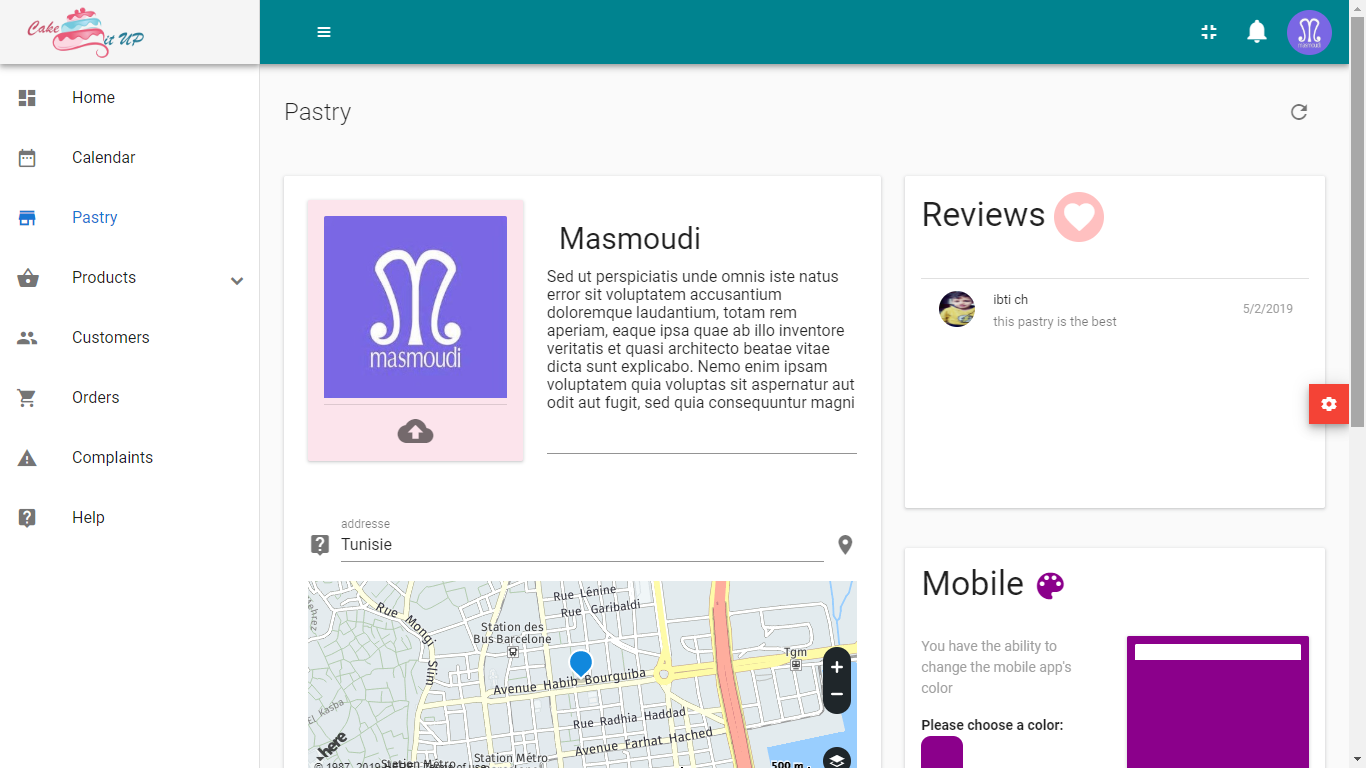
\includegraphics[width=6in,keepaspectratio]{edit-pastry.png}
	\caption{Edit pastry interface web}
	\label{editpastry-interface}
\end{figure} 

\subsubsection*{Sprint "Manage products"}
Figure \ref{productlist-interface} gives us an idea about what the list of product look like in the web application, the list is click-able, a click will take you to the specific product, you can also access the edit mode and archive a product from it.
\begin{figure}[H]
	\centering
	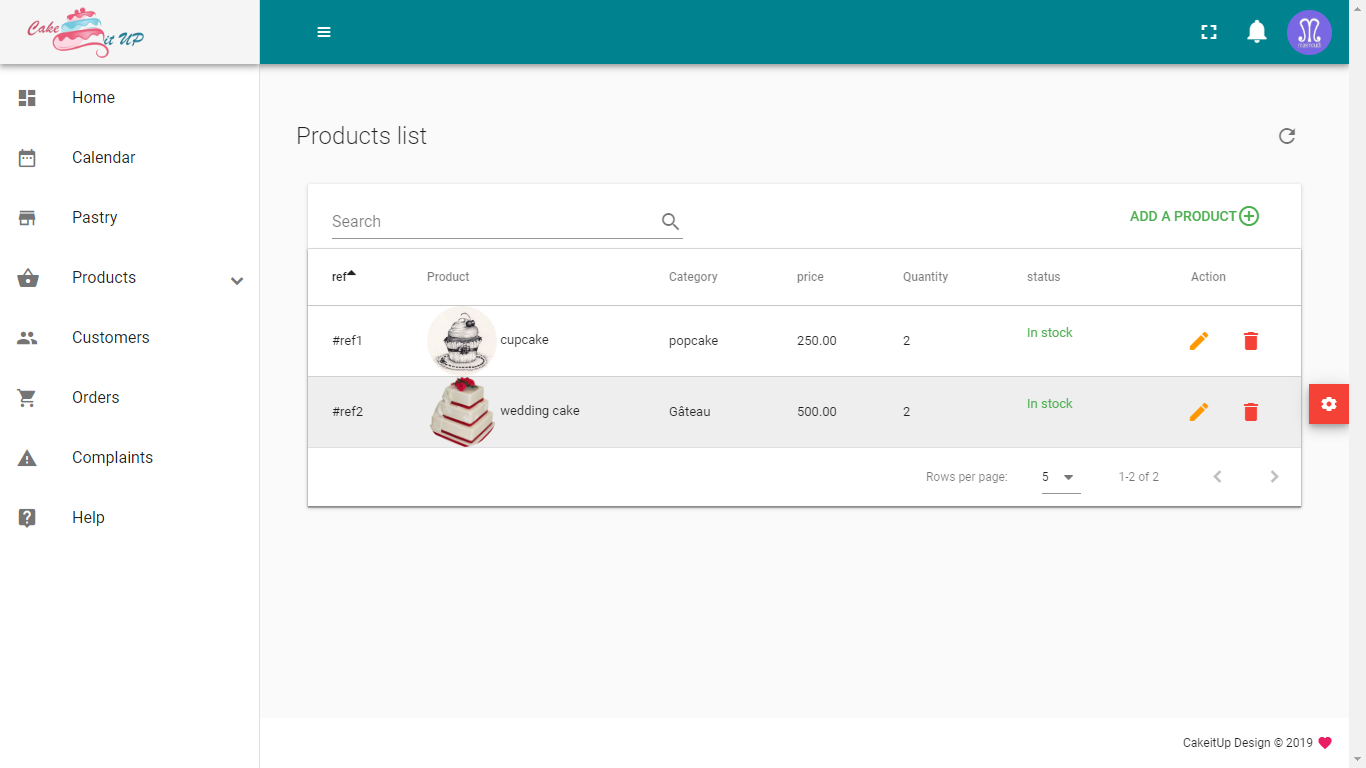
\includegraphics[width=6in,keepaspectratio]{productlist.png}
	\caption{Product list interface web}
	\label{productlist-interface}
\end{figure} 
Adding a product can be found only on the web side where a pastry owner can describe his product and fill in all the forms.
\begin{figure}[H]
	\centering
	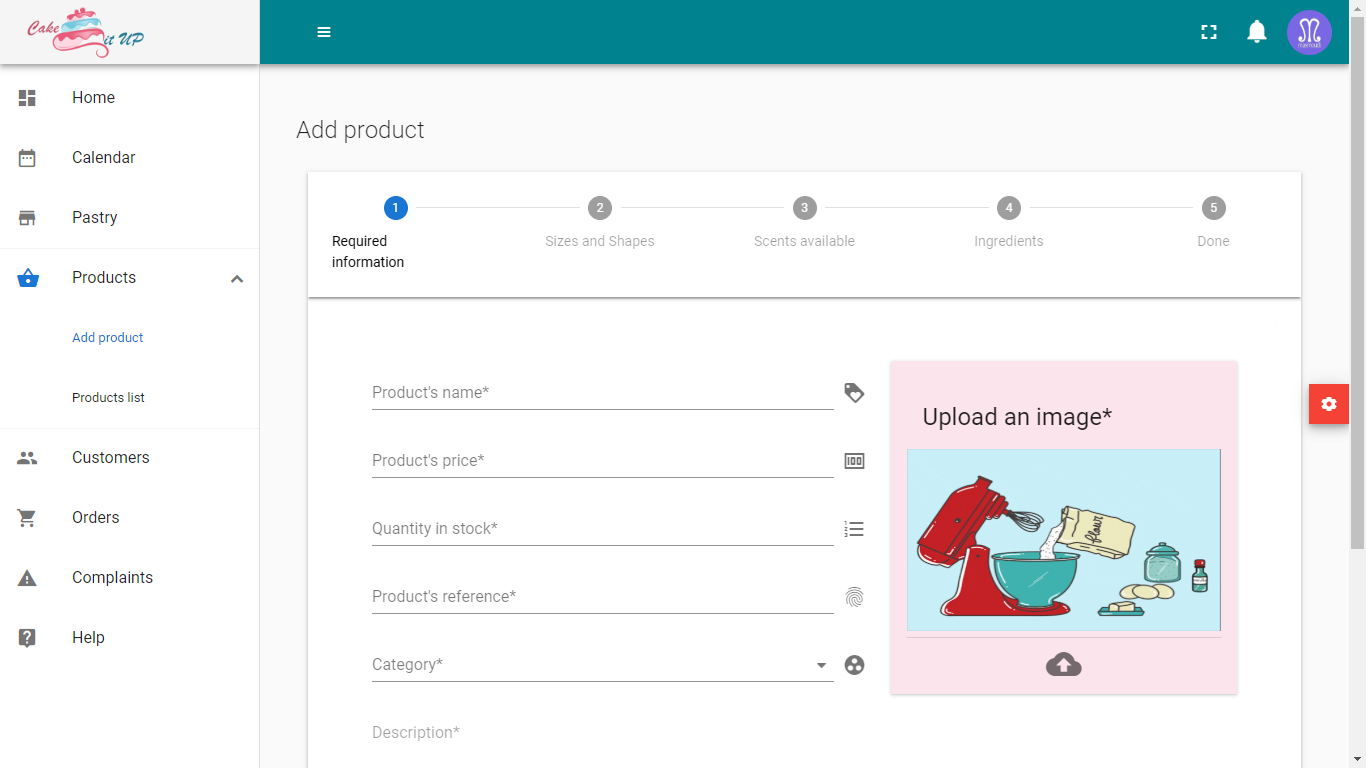
\includegraphics[width=5.5in,keepaspectratio]{addproduct.png}
	\caption{Add product interface}
	\label{addproduct-interface}
\end{figure} 
The pastry owner can edit his product and change any information he wants as long as it is valid.
\begin{figure}[H]
	\vspace*{1in}
	\centering
	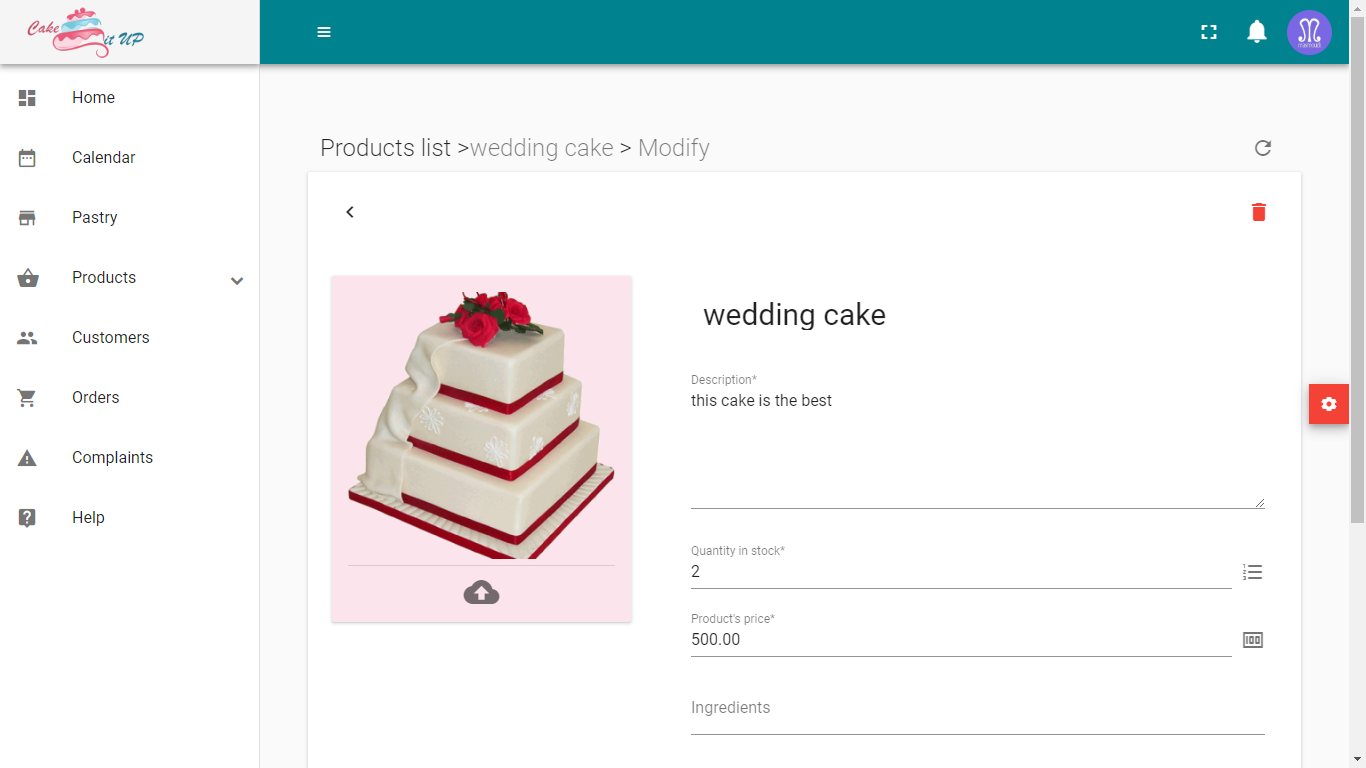
\includegraphics[width=7in,keepaspectratio]{editproduct.png}
	\caption{Edit product interface}
	\label{editproduct-interface}
\end{figure} 
\clearpage
\subsection{mobile}
\subsubsection*{Sprint "Authentication"}
The client won't have access to his profile unless he loges in, the interface shown in Figure \ref{accountnonconnect-mobile-interface} presents the layout showed when the user is a visitor.

\begin{figure}[H]
	\vspace*{1in}
	\centering
	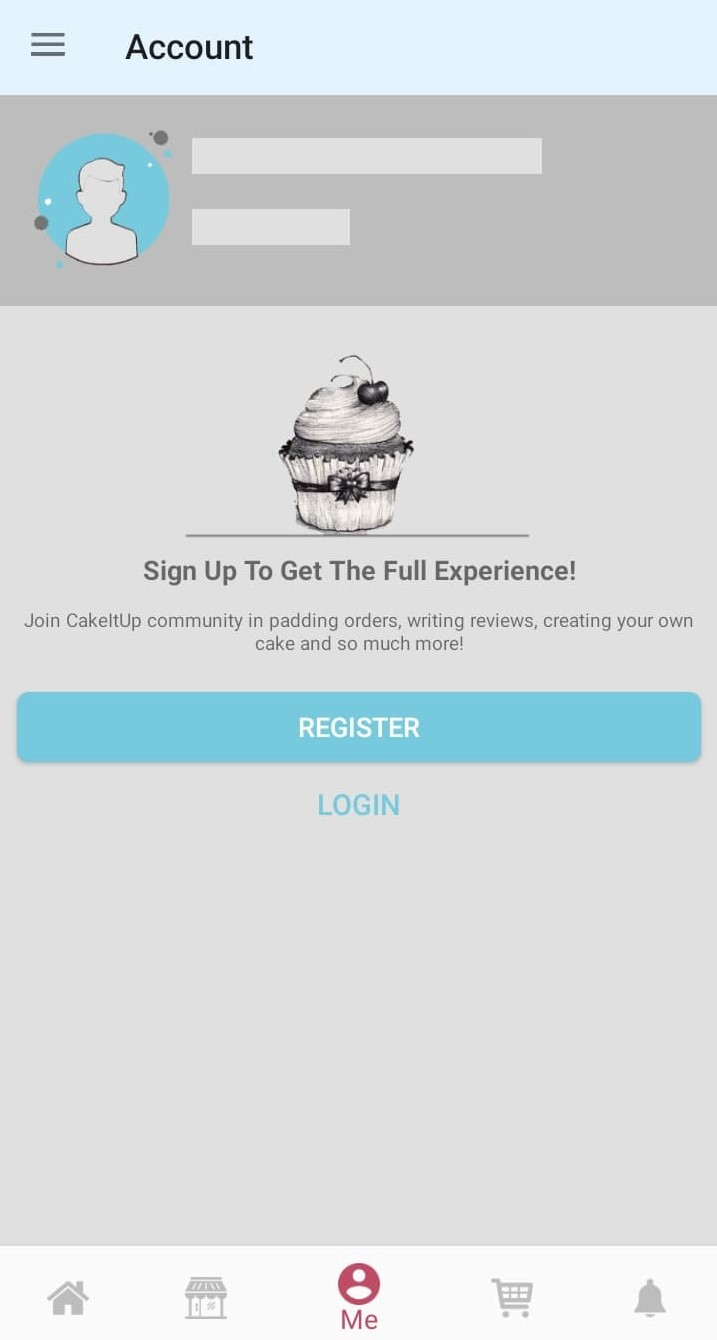
\includegraphics[width=3in,keepaspectratio]{accountnotconnectedlogin.jpg}
	\caption{Profile non connected mobile interface}
	\label{accountnonconnect-mobile-interface}
\end{figure} 

\clearpage
To create an account, the client just needs to fill in the form show in Figure \ref{auth-label}.\par 
Once the account is created, the client can login by filling in the valid information.
\begin{figure}[H]
	\centering
	\vspace*{1in}
	\subfloat[Register interface]{{\includegraphics[width=7cm]{registermobile.jpg} }}%
	\qquad
	\subfloat[Login interface]{{\includegraphics[width=7cm]{loginmobile.jpg} }}%
	\caption{Register and login mobile interface}%
	\label{auth-label}%
\end{figure}
\clearpage
\subsubsection*{Sprint "Manage account"}
Once the use is logged in he have access to his own profile where he can find his personal information.\par
The client can edit his profile as shown in Figure \ref{manageaccount-label}.
\begin{figure}[H]
	\centering
	\vspace*{1in}
	\subfloat[Register interface]{{\includegraphics[width=7cm]{profilemobile.jpg} }}%
	\qquad
	\subfloat[Login interface]{{\includegraphics[width=7cm]{editprofilemobile.jpg} }}%
	\caption{Register and login mobile interface}%
	\label{manageaccount-label}%
\end{figure}

\clearpage
Resetting a password has the same process as the web application.
\begin{figure}[H]
			\vspace*{1in}
	\centering
	\includegraphics[width=3in,keepaspectratio]{resetpasswordmobile.jpg}
	\caption{Reset password mobile interface}
	\label{resetpasswordmobile-interface}
\end{figure}
\clearpage
\subsubsection*{Sprint "Manage pastries"}
The list of pastries is accessible to all users the only difference is that some function are not allowed if you are not logged in.\par 
A single pastry can be viewed by clicking on one of the pastries in the list.
\begin{figure}[H]
	\centering
	\vspace*{1in}
	\subfloat[Register interface]{{\includegraphics[width=7cm]{pastriesListmobile.jpg} }}%
	\qquad
	\subfloat[Login interface]{{\includegraphics[width=7cm]{showpastrymobile.jpg} }}%
	\caption{Register and login mobile interface}%
	\label{managepastries-label}%
\end{figure}


\section{Release retrospective}
	After the first sprint, we did the tests to see if
	we were able to achieve the goals set out. And for that, we rely on the
	sprint retrospective:\\
	\begin{itemize}
		\item	What went well:
	\begin{itemize}
		\item The tasks of this module went well. There were no problems
		in this sprint.
	\end{itemize}
\end{itemize}
\begin{itemize}
	\item	What went wrong:
	\begin{itemize}
		\item Nothing.
	\end{itemize}
\end{itemize}
\begin{itemize}
	\item	What was not realized:
	\begin{itemize}
		\item Nothing.
	\end{itemize}
\end{itemize}
	\begin{itemize}
	\item	What can be improved:
	\begin{itemize}
		\item the presentation of the interfaces can be improved,
		\item the validation of the form authentication can be enriched more.
	\end{itemize}
	\end{itemize}
 
	\section*{Conclusion}
	\addcontentsline{toc}{section}{Conclusion}
	At the end of this chapter, we have managed to produce a work with sufficient value for the customer and can be used in a production environment. In the following chapter, our effort will be devoted to the production of a new release.
	\chapter{Release 2}
	\section*{Introduction}
	\addcontentsline{toc}{section}{Introduction}
	According to the established plan, the second Sprint focuses on the use cases: "Manage clients", "Manage complains", "Manage reports" and "Manage events".
	\section{Backlog}
	\begin{table}[H]
		\begin{center}
			\captionsetup[table]{skip=10pt}
			\caption{Backlog: Release 2}
			\setlength\doublerulesep{0.5pt}
			\begin{tabular}{|  p{3cm}|  p{1cm}| p{4cm}|  p{1cm}| p{6cm}|}
				\hline 
				\rowcolor{LightCyan}
				\textbf{Sprint} & \textbf{ID \ac{us}} & \textbf{User story} & \textbf{ID task} & \textbf{Task} 
				\\
				\hline
				\multirow{5}{3cm}{\textbf{Sprint 9} \textbf{Manage clients} }
				&                       
				9.1  &  
				\multirow{2}{4cm}{As an administrator i want to view list of all clients.}
				
				&				                      
				9.1.A &                        
				Make the diagrams needed for this \ac{us} (use case diagram, class diagram, sequence diagram).
				\\ 
				\cline{4-5}    
				&                   
				&                                 
				&                        
				9.1.B &                        
				Develop the view list of clients model for the administrator.
				\\ 
				\cline{4-5}    
				&                   
				&                                 
				&                        
				9.1.C &                        
				Test the list of clients model.
				\\
				\cline{2-5}  
				
				&                       
				5.2  &  
				\multirow{2}{4cm}{As an administrator i want to block a client.}
				
				&				                      
				9.2.A &                        
				Make the diagrams needed for this \ac{us}.
				\\ 
				\cline{4-5}    
				&                   
				&                                 
				&                        
				9.2.B &                        
				Develop the block client model.
				
				
				
				
				
			\end{tabular}
			
		\end{center}
		
	\end{table}
	\begin{table}[H]
	\begin{center}
		\setlength\doublerulesep{0.5pt}
		\begin{tabular}{|  p{3cm}|  p{1cm}| p{4cm}|  p{1cm}| p{6cm}|}
	
			\cline{4-5}    
			&                   
			&                                 
			&                        
			5.2.C &                        
			Test the block client model.
			\\
			\cline{2-5}  
			
			&                       
			5.3  &  
			\multirow{2}{4cm}{As a pastry owner i want to view list of my clients.}
			
			&				                      
			5.3.A &                        
			Make the diagrams needed for this \ac{us}.
			\\ 
			\cline{4-5}    
			&                   
			&                                 
			&                        
			5.3.B &                        
			Develop the list of clients model for the pastry owner.
			\\ 
			\cline{4-5}    
			&                   
			&                                 
			&                        
			5.3.C &                        
			Test the list of clients model.
				\\
			\hline
			\multirow{5}{3cm}{\textbf{Sprint 6} \textbf{Manage Complains} }
			&                       
			6.1  &  
			\multirow{2}{4cm}{As a client i want to add a complain.}
			
			&				                      
			6.1.A &                        
			Make the diagrams needed for this \ac{us} (use case diagram, class diagram, sequence diagram).
			\\ 
			\cline{4-5}    
			&                   
			&                                 
			&                        
			6.1.B &                        
			Develop the add complain model.
			\\ 
			\cline{4-5}    
			&                   
			&                                 
			&                        
			6.1.C &                        
			Test the add complain model.
			\\
			\cline{2-5}  
			
			&                       
			6.2  &  
			\multirow{2}{4cm}{As a client i wnat to view my list of complains.}
			
			&				                      
			6.2.A &                        
			Make the diagrams needed for this \ac{us}.
			\\ 
			\cline{4-5}    
			&                   
			&                                 
			&                        
			6.2.B &                        
			Develop the complains list model.
			\\ 
			\cline{4-5}    
			&                   
			&                                 
			&                        
			6.2.C &                        
			Test the complains list model.
			\\
			\cline{2-5}  
			
			&                       
			6.3  &  
			\multirow{2}{4cm}{As a pastry owner i want to view the list of complains.}
			
			&				                      
			6.3.A &                        
			Make the diagrams needed for this \ac{us}.
			\\ 
			\cline{4-5}    
			&                   
			&                                 
			&                        
			6.3.B &                        
			Develop the list of complains model.
			\\ 
			\cline{4-5}    
			&                   
			&                                 
			&                        
			6.3.C &                        
			Test the complains list model.
			\\
			\cline{2-5}  
			
			&                       
			6.4  &  
			\multirow{2}{4cm}{As a pastry owner i want to reply to a complain.}
			
			&				                      
			6.4.A &                        
			Make the diagrams needed for this \ac{us}.
			\\ 
			\cline{4-5}    
			&                   
			&                                 
			&                        
			6.4.B &                        
			Develop the reply model.
			\\ 
			\cline{4-5}    
			&                   
			&                                 
			&                        
			6.4.C &                        
			Test the reply to complain model.
				\\
			\hline
			\multirow{5}{3cm}{\textbf{Sprint 7} \textbf{Manage reports} }
			&                       
			7.1  &  
			\multirow{2}{4cm}{As a client i want to report a pastry.}
			
			&				                      
			7.1.A &                        
			Make the diagrams needed for this \ac{us} (use case diagram, class diagram, sequence diagram).
			\\ 
			\cline{4-5}    
			&                   
			&                                 
			&                        
			7.1.B &                        
			Develop the add report model.
			\\ 
			\cline{4-5}    
			&                   
			&                                 
			&                        
			7.1.C &                        
			Test the add report model.
			
			
			
		\end{tabular}
		
	\end{center}
	
\end{table}
	\begin{table}[H]
	\begin{center}
		\setlength\doublerulesep{0.5pt}
		\begin{tabular}{|  p{3cm}|  p{1cm}| p{4cm}|  p{1cm}| p{6cm}|}
		
			\cline{2-5}  
			
			&                       
			7.2  &  
			\multirow{2}{4cm}{As a pastry owner i want to report a client.}
			
			&				                      
			7.2.A &                        
			Make the diagrams needed for this \ac{us}.
			\\ 
			\cline{4-5}    
			&                   
			&                                 
			&                        
			7.2.B &                        
			Develop the add report model.
			\\ 
			\cline{4-5}    
			&                   
			&                                 
			&                        
			7.2.C &                        
			Test the add report model.
			\\
			\cline{2-5}  
			
			&                       
			7.3  &  
			\multirow{2}{4cm}{As an administrator i want to view list of reports.}
			
			&				                      
			7.3.A &                        
			Make the diagrams needed for this \ac{us}.
			\\ 
			\cline{4-5}    
			&                   
			&                                 
			&                        
			7.3.B &                        
			Develop the list of reports model.
			\\ 
			\cline{4-5}    
			&                   
			&                                 
			&                        
			7.3.C &                        
			Test the reports list model.
			\\
			\hline
			\multirow{5}{3cm}{\textbf{Sprint 8} \textbf{Manage events} }
			&                       
			8.1  &  
			\multirow{2}{4cm}{As a pastry owner i want to add a personal event.}
			
			&				                      
			8.1.A &                        
			Make the diagrams needed for this \ac{us} (use case diagram, class diagram, sequence diagram).
			\\ 
			\cline{4-5}    
			&                   
			&                                 
			&                        
			8.1.B &                        
			Develop the add event model.
			\\ 
			\cline{4-5}    
			&                   
			&                                 
			&                        
			8.1.C &                        
			Test the add event model.
			\\
			\cline{2-5}  
			
			&                       
			8.2  &  
			\multirow{2}{4cm}{As a pastry owner i want to view my calender.}
			
			&				                      
			8.2.A &                        
			Make the diagrams needed for this \ac{us}.
			\\ 
			\cline{4-5}    
			&                   
			&                                 
			&                        
			8.2.B &                        
			Develop the calender model.
			\\ 
			\cline{4-5}    
			&                   
			&                                 
			&                        
			8.2.C &                        
			Test the calender model.
			
			\\
			\hline
		\end{tabular}
		
	\end{center}
	
\end{table}
\clearpage
	\section{Use case}
	\subsection{Use case diagram}
	We will be following the same steps as the previous release, starting by the use case of the first sprint of this release \textbf{``Manage clients''} presented in Figure \ref{clients-diag}.
	\begin{figure}[H]
		\vspace*{1cm}
		\centering
		\includegraphics[width=7.2in,keepaspectratio]{manageClients.png}
		\caption{Use case Manage clients}
		\label{clients-diag}
	\end{figure}
As for the second sprint \textbf{``Manage complains''}, we created another use case diagram showing in Figure \ref{complains-diag}
\begin{figure}[H]
	\vspace*{2cm}
	\centering
	\includegraphics[width=7in,keepaspectratio]{manageComplains.png}
	\caption{Use case Manage complains}
	\label{complains-diag}
\end{figure}
\clearpage
 Sprint \textbf{``Manage complains''} which is the third sprint this this release is presented in Figure \ref{reports-diag}.
 
\begin{figure}[H]
	\centering
	\includegraphics[width=5.4in,keepaspectratio]{manageReports.png}
	\caption{Use case Manage reports}
	\label{reports-diag}
\end{figure}

The last sprint in this release is \textbf{``Manage events''}, Figure \ref{events-diag} is a use case diagram that describes the different cases of this sprint.
\begin{figure}[H]
	\centering
	\includegraphics[width=5.4in,keepaspectratio]{manageEvents.png}
	\caption{Use case Manage events}
	\label{events-diag}
\end{figure}
	\subsection{Use case description}
	We will be description each and every use case of this release in this section.
	\subsubsection*{Use case "Manage clients" description}
	\begin{table}[H]
		\begin{center}
			\captionsetup[table]{skip=10pt}
			\caption{Use case "Manage clients" description}
			\setlength\doublerulesep{0.5pt}
			\begin{tabular}{|  p{5cm}|  p{9cm}|}
				\rowcolor{LightCyan}
				
				\hline
				\multicolumn{2}{c}{Use case "Manage clients"}\\
				\hline
				
				\textbf{Actors} &                        
				Administrator and pastry owner 
				\\ \hline
				
				\textbf{Precondition} &                        
				Clients exists and the actors are authenticated and authorized
				\\ \hline
				\textbf{Postcondition} &                        
				Clients viewed or blocked
				\\ \hline
				
				\textbf{Main scenario} &                        
				\begin{itemize}
					\item block client,
						\begin{itemize}
						\item the administrator block a client,
						\item The system save changes.
					\end{itemize}
					\item view list of clients.
				
				\begin{itemize}
					\item the actor access the list of clients,
					\item The actor sort, search or select a client from the list.
				\end{itemize}
			\end{itemize}
				\\ \hline
				
				\textbf{Alternative scenario} &                        
				In case of an error the system will show an error message.
				\\ \hline
				
				
			\end{tabular}
			
		\end{center}
		
	\end{table}
	\subsubsection*{Use case "Manage complains" description}
		\begin{table}[H]
		\begin{center}
			\captionsetup[table]{skip=10pt}
			\caption{Use case "Manage complains" description}
			\setlength\doublerulesep{0.5pt}
			\begin{tabular}{|  p{5cm}|  p{9cm}|}
				\rowcolor{LightCyan}
				
				\hline
				\multicolumn{2}{c}{Use case "Manage complains"}\\
				\hline
				
				\textbf{Actors} &                        
			The pastry owner and the client
				\\ \hline
				
				\textbf{Precondition} &                        
				the actors are authorized and authenticated
				\\ \hline
				\textbf{Postcondition} &                        
				A complain is created or updated
				\\ \hline
				
				\textbf{Main scenario} &                        
				\begin{itemize}
					\item Add complain,
					\begin{itemize}
						\item the client will send a complain to a specific pastry,
						\item The system save the complain.
						\item The pastry owner will receive the complain.
					\end{itemize}
					\item Reply to a complain.
					
					\begin{itemize}
						\item the pastry owner will reply to the complain,
						\item The system update the complain.
						\item The client will receive the reply.
					\end{itemize}
				\end{itemize}
				\\ \hline
				
				\textbf{Alternative scenario} &                        
				In case of an error the system will show an error message.
				\\ \hline
				
				
			\end{tabular}
			
		\end{center}
		
	\end{table}
	\subsubsection*{Use case "Manage reports" description}
		\begin{table}[H]
		\begin{center}
			\captionsetup[table]{skip=10pt}
			\caption{Use case "Manage reports" description}
			\setlength\doublerulesep{0.5pt}
			\begin{tabular}{|  p{5cm}|  p{9cm}|}
				\rowcolor{LightCyan}
				
				\hline
				\multicolumn{2}{c}{Use case "Manage reports"}\\
				\hline
				
				\textbf{Actors} &                        
				The user
				\\ \hline
				
				\textbf{Precondition} &                        
				the actors are authorized and authenticated
				\\ \hline
				\textbf{Postcondition} &                        
				A report is created or viewed
				\\ \hline
				
				\textbf{Main scenario} &                        
				\begin{itemize}
					\item Add report,
					\begin{itemize}
						\item a client or a pastry owner can report each other,
						\item The system save the report.
					\end{itemize}
					\item view reports
					
					\begin{itemize}
						\item the administrator view the list of reports
					\end{itemize}
				\end{itemize}
				\\ \hline
				
				\textbf{Alternative scenario} &                        
				In case of an error the system will show an error message.
				\\ \hline
				
				
			\end{tabular}
			
		\end{center}
		
	\end{table}
	\subsubsection*{Use case "Manage events" description}
	\begin{table}[H]
		\begin{center}
			\captionsetup[table]{skip=10pt}
			\caption{Use case "Manage events" description}
			\setlength\doublerulesep{0.5pt}
			\begin{tabular}{|  p{5cm}|  p{9cm}|}
				\rowcolor{LightCyan}
				
				\hline
				\multicolumn{2}{c}{Use case "Manage events"}\\
				\hline
				
				\textbf{Actors} &                        
				The pastry owner
				\\ \hline
				
				\textbf{Precondition} &                        
				the pastry owner is authenticated
				\\ \hline
				\textbf{Postcondition} &                        
				An event is created or viewed
				\\ \hline
				
				\textbf{Main scenario} &                        
				\begin{itemize}
					\item Add event,
					\begin{itemize}
						\item The pastry owner create an event,
						\item The system save the event.
					\end{itemize}
					\item view reports
					
					\begin{itemize}
						\item The pastry owner view his calender with the list of events
					\end{itemize}
				\end{itemize}
				\\ \hline
				
				\textbf{Alternative scenario} &                        
				In case of an error the system will show an error message.
				\\ \hline
				
				
			\end{tabular}
			
		\end{center}
		
	\end{table}

\section{Sequence diagram}
The same as the previous release will be dedicating this section for the sequence diagrams.\par 
We have four sprint and we will be presenting only two of them to give an idea about the work flow of our application.
\subsubsection*{Sequence diagram "Manage complains"}
In the third sprint of this release which is \textbf{Manage complains} we have two actors with two different applications but the same database.\par 
Figure \ref{complains-sequence} is giving us a detailed description of the way our system works. Since we have two different application, means we have two different work flow, for the web part it is \ac{mvc} where the user have an interaction with the view and the view with the controller and the controller with the database. The mobile application is based on \ac{mvp} where the user interacts with presented and this last with the repository and the repository with the database.\par

\begin{figure}[H]
	\centering
	\includegraphics[width=7in,height=8in]{managecomplains.jpg}
	\caption{Manage complains sequence diagram}
	\label{complains-sequence}
\end{figure}
\clearpage
\subsubsection*{Sequence diagram "Manage reports"}
Figure \ref{reports-sequence} is a representation of the needed steps to the third sprint of this release, the actors are all involved in this sprint to either view list of reports for the administrator, or reporting a pastry for the client, or reporting a pastry for the pastry owner.
\begin{figure}[H]
	\centering
	\includegraphics[width=7in,height=7.5in]{managerepors.jpg}
	\caption{Manage reports sequence diagram}
	\label{reports-sequence}
\end{figure}
\clearpage
	\section{Implementation}
	In this section we will present our interfaces for the four sprints in this release.
\subsection{Web}
\subsubsection*{Sprint "Manage clients"}
Sprint manage clients has three different tasks where the administrator can view the list of clients as shown in Figure \ref{listclients-interface}, via this interface he can also block a client.
\begin{figure}[H]
	\centering
	\vspace*{1in}
	\includegraphics[width=7in,keepaspectratio]{listclients.png}
	\caption{List of clients interface web}
	\label{listclients-interface}
\end{figure} 
\clearpage
\subsubsection*{Sprint "Manage complains"}
The pastry owner can view the complains that were send by their clients.
\begin{figure}[H]
	\centering
	\includegraphics[width=5.6in,keepaspectratio]{complainslist.png}
	\caption{List of complains interface web}
	\label{complainslist-interface}
\end{figure}
He can also reply to a complain as shown in Figure \ref{replytocomplain-interface}.
\begin{figure}[H]
	\centering
	\includegraphics[width=5.6in,keepaspectratio]{replytocomplain.png}
	\caption{Reply to complain interface web}
	\label{replytocomplain-interface}
\end{figure}

\subsubsection*{Sprint "Manage reports"}
The reports do not really have that much to be done on but they are really important, the administrator is the only user authorized to access the list of reports.
\begin{figure}[H]
	\centering
	\includegraphics[width=5.6in,keepaspectratio]{listreports.png}
	\caption{List of reports interface web}
	\label{listreports-interface}
\end{figure}

\subsubsection*{Sprint "Manage events"}
The events or orders can be view in the calender interface as shown in Figure \ref{listevents-interface}.
\begin{figure}[H]
	\centering
	\includegraphics[width=5.6in,keepaspectratio]{listevents.png}
	\caption{Calender interface web}
	\label{listevents-interface}
\end{figure}
To add an event all the user has to do is fill in the form that is shown in Figure \ref{addevent-interface}.
\begin{figure}[H]
	\vspace*{1in}
	\centering
	\includegraphics[width=7in,keepaspectratio]{addevent.png}
	\caption{Add event interface web}
	\label{addevent-interface}
\end{figure}
\clearpage
\subsection{Mobile}
\subsubsection*{Sprint "Manage account"}
The client has access to his own list of complain that he has already sent to a number of pastries, The Figure \ref{listcomplainsmobile-interface} gives us an idea about how this layout look like.
\begin{figure}[H]
	\centering
	\includegraphics[width=3in,keepaspectratio]{listcomplainsmobile.jpg}
	\caption{List of complains mobile interface}
	\label{listcomplainsmobile-interface}
\end{figure}
\clearpage
	\section{Release retrospective}
		Finishing this release, we had to test every sprint where we decided on these retrospectives:\\
	\begin{itemize}
		\item	What went well:
		\begin{itemize}
			\item The tasks of this module went well. There were no problems
			in this sprint.
		\end{itemize}
	\end{itemize}
	\begin{itemize}
		\item	What went wrong:
		\begin{itemize}
			\item Nothing.
		\end{itemize}
	\end{itemize}
	\begin{itemize}
		\item	What was not realized:
		\begin{itemize}
			\item Nothing.
		\end{itemize}
	\end{itemize}
	\begin{itemize}
		\item	What can be improved:
		\begin{itemize}
			\item the presentation of the interfaces can be improved
		\end{itemize}
	\end{itemize}
	\section*{Conclusion}
	\addcontentsline{toc}{section}{Conclusion}
	In this chapter, we presented the second sprint result. And like the first sprint we went through specification, design, coding and retrospectives. In the last chapter our effort will be devoted to producing the third and last sprint.
	
	\chapter{Release 3}
	\section*{Introduction}
	\addcontentsline{toc}{section}{Introduction}
	We start from the same principle as the previous sprint, but this time we focus on the following use cases: "Manage reviews", "Manage rating", "Manage cart", "Manage orders" and "Manage personal orders".\par 
	Our goal is to have, at the end of this sprint, a version of the application that is stable.
	\section{Backlog}
	\begin{table}[H]
		\begin{center}
			\captionsetup[table]{skip=10pt}
			\caption{Backlog: Release 3}
			\setlength\doublerulesep{0.5pt}
			\begin{tabular}{|  p{3cm}|  p{1cm}| p{4cm}|  p{1cm}| p{6cm}|}
				\hline 
				\rowcolor{LightCyan}
				\textbf{Sprint} & \textbf{ID \ac{us}} & \textbf{User story} & \textbf{ID task} & \textbf{Task} 
				\\
				\hline
				\multirow{5}{3cm}{\textbf{Sprint 9} \textbf{Manage reviews} }
				&                       
				9.1  &  
				\multirow{2}{4cm}{As a client i want to add a review.}
				
				&				                      
				9.1.A &                        
				Make the diagrams needed for this \ac{us} (use case diagram, class diagram, sequence diagram).
				\\ 
				\cline{4-5}    
				&                   
				&                                 
				&                        
				9.1.B &                        
				Develop the add review model.
				\\ 
				\cline{4-5}    
				&                   
				&                                 
				&                        
				9.1.C &                        
				Test the add review model.
				
				
				
				
			\end{tabular}
			
		\end{center}
		
	\end{table}
\begin{table}[H]
	\begin{center}

		\setlength\doublerulesep{0.5pt}
		\begin{tabular}{|  p{3cm}|  p{1cm}| p{4cm}|  p{1cm}| p{6cm}|}
			\cline{2-5}  
			
			&                       
			9.2  &  
			\multirow{2}{4cm}{As a pastry owner i want to view my pastry's review.}
			
			&				                      
			9.2.A &                        
			Make the diagrams needed for this \ac{us}.
			\\ 
			\cline{4-5}    
			&                   
			&                                 
			&                        
			9.2.B &                        
			Develop the list of reviews model.
			
			\\ 
			\cline{4-5}    
			&                   
			&                                 
			&                        
			9.2.C &                        
			Develop the list of reviews model.
			\\
			\hline
			\multirow{5}{3cm}{\textbf{Sprint 10} \textbf{Manage ratings} }
			&                       
			10.1  &  
			\multirow{2}{4cm}{As a client i want to rate a pastry.}
			
			&				                      
			10.1.A &                        
			Make the diagrams needed for this \ac{us} (use case diagram, class diagram, sequence diagram).
			\\ 
			\cline{4-5}    
			&                   
			&                                 
			&                        
			10.1.B &                        
			Develop the rate pastry model.
			\\ 
			\cline{4-5}    
			&                   
			&                                 
			&                        
			10.1.C &                        
			Test the rate pastry model.
			\\
			\cline{2-5}  
			
			&                       
			10.2  &  
			\multirow{2}{4cm}{As a pastry owner i want to view my pastry's rating.}
			
			&				                      
			10.2.A &                        
			Make the diagrams needed for this \ac{us}.
			\\ 
			\cline{4-5}    
			&                   
			&                                 
			&                        
			10.2.B &                        
			Develop the view rating model.
			\\ 
			\cline{4-5}    
			&                   
			&                                 
			&                        
			10.2.C &                        
			Test the view rating model.
			\\
			\hline
			\multirow{5}{3cm}{\textbf{Sprint 11} \textbf{Statistics} }
			&                       
			11.1  &  
			\multirow{2}{4cm}{As an administrator or a pastry owner i want to view statistics.}
			
			&				                      
			11.1.A &                        
			Make the diagrams needed for this \ac{us} (use case diagram, class diagram, sequence diagram).
			\\ 
			\cline{4-5}    
			&                   
			&                                 
			&                        
			11.1.B &                        
			Develop the statistics model.
			\\ 
			\cline{4-5}    
			&                   
			&                                 
			&                        
			11.1.C &                        
			Test the statistics model.
		\\
		\hline
		\multirow{5}{3cm}{\textbf{Sprint 12} \textbf{Manage cart} }
		&                       
		12.1  &  
		\multirow{2}{4cm}{As a client i want to edit my own cart.}
		
		&				                      
		12.1.A &                        
		Make the diagrams needed for this \ac{us} (use case diagram, class diagram, sequence diagram).
		\\ 
		\cline{4-5}    
		&                   
		&                                 
		&                        
		12.1.B &                        
		Develop the edit cart model.
		\\ 
		\cline{4-5}    
		&                   
		&                                 
		&                        
		12.1.C &                        
		Test the edit cart model.
		\\
		\cline{2-5}  
		
		&                       
		12.2  &  
		\multirow{2}{4cm}{As a client i want to view my cart.}
		
		&				                      
		12.2.A &                        
		Make the diagrams needed for this \ac{us}.
		\\ 
		\cline{4-5}    
		&                   
		&                                 
		&                        
		12.2.B &                        
		Develop the view cart model.
		\\ 
		\cline{4-5}    
		&                   
		&                                 
		&                        
		12.2.C &                        
		Test the view cart model.
	
		\end{tabular}
		
	\end{center}
	
\end{table}
\begin{table}[H]
	\begin{center}
		
		\setlength\doublerulesep{0.5pt}
		\begin{tabular}{|  p{3cm}|  p{1cm}| p{4cm}|  p{1cm}| p{6cm}|}
			
			\hline
			\multirow{5}{3cm}{\textbf{Sprint 13} \textbf{Manage orders} }
			&                       
			13.1  &  
			\multirow{2}{4cm}{As a client i want to pass an order.}
			
			&				                      
			13.1.A &                        
			Make the diagrams needed for this \ac{us} (use case diagram, class diagram, sequence diagram).
			\\ 
			\cline{4-5}    
			&                   
			&                                 
			&                        
			13.1.B &                        
			Develop the pass order model.
			\\ 
			\cline{4-5}    
			&                   
			&                                 
			&                        
			13.1.C &                        
			Test the pass order model.
			\\
			\cline{2-5}  
			
			&                       
			13.2  &  
			\multirow{2}{4cm}{As a client i want to view my own orders.}
			
			&				                      
			13.2.A &                        
			Make the diagrams needed for this \ac{us}.
			\\ 
			\cline{4-5}    
			&                   
			&                                 
			&                        
			13.2.B &                        
			Develop the view orders model.
			\\ 
			\cline{4-5}    
			&                   
			&                                 
			&                        
			13.2.C &                        
			Test the view orders model.
			\\
			\cline{2-5}  
			
			&                       
			13.3  &  
			\multirow{2}{4cm}{As a pastry owner i want to view orders.}
			
			&				                      
			13.3.A &                        
			Make the diagrams needed for this \ac{us}.
			\\ 
			\cline{4-5}    
			&                   
			&                                 
			&                        
			13.3.B &                        
			Develop the view orders model.
			\\ 
			\cline{4-5}    
			&                   
			&                                 
			&                        
			13.3.C &                        
			Test the view orders model.
			\\
			\cline{2-5}  
			
			&                       
			13.4  &  
			\multirow{2}{4cm}{As a pastry owner i want to change the state of an order.}
			
			&				                      
			13.4.A &                        
			Make the diagrams needed for this \ac{us}.
			\\ 
			\cline{4-5}    
			&                   
			&                                 
			&                        
			13.4.B &                        
			Develop the change state of order model.
			\\ 
			\cline{4-5}    
			&                   
			&                                 
			&                        
			13.4.C &                        
			Test the change state of order model.
			\\
			\hline
			\multirow{5}{3cm}{\textbf{Sprint 14} \textbf{Manage personal orders} }
			&                       
			14.1  &  
			\multirow{2}{4cm}{As a client i want to add a personal order.}
			
			&				                      
			14.1.A &                        
			Make the diagrams needed for this \ac{us} (use case diagram, class diagram, sequence diagram).
			\\ 
			\cline{4-5}    
			&                   
			&                                 
			&                        
			14.1.B &                        
			Develop the add personal order model.
			\\ 
			\cline{4-5}    
			&                   
			&                                 
			&                        
			14.1.C &                        
			Test the  add personal order model.
			\\
			\cline{2-5}  
			
			&                       
			14.2  &  
			\multirow{2}{4cm}{As a client i want to view my list of personal orders.}
			
			&				                      
			14.2.A &                        
			Make the diagrams needed for this \ac{us}.
			\\ 
			\cline{4-5}    
			&                   
			&                                 
			&                        
			14.2.B &                        
			Develop the view list of personal orders model.
			\\ 
			\cline{4-5}    
			&                   
			&                                 
			&                        
			14.2.C &                        
			Test the list of personal orders model.
			
			\\
			\hline
		\end{tabular}
		
	\end{center}
	
\end{table}
	\section{Use case}
		\subsection{Use case diagrams}
		We are dedicating this section to present the use case diagrams for this release.\par 
		Starting by the first sprint of this release \textbf{Manage reviews} which is illustrator in Figure \ref{ratings-usecase}.
		\begin{figure}[H]
			
			\centering
			\includegraphics[width=5in,keepaspectratio]{manageReviews.png}
			\caption{Manage reviews use case}
			\label{reviews-usecase}
		\end{figure}
	The next use case diagram to be presented is \textbf{Manage ratings} shown in Figure \ref{ratings-usecase}.
	\begin{figure}[H]
		
		\centering
		\includegraphics[width=5in,keepaspectratio]{manageratings.png}
		\caption{Manage ratings use case}
		\label{ratings-usecase}
	\end{figure}
Figure \ref{statistics-usecase} presents the use case for the sprint  \textbf{Statistics}.
\begin{figure}[H]
	\vspace*{2cm}
	\centering
	\includegraphics[width=7in,keepaspectratio]{statistics.png}
	\caption{Statistics use case}
	\label{statistics-usecase}
	
\end{figure}
\clearpage
As for the sprint \textbf{Manage cart} we created the use case presented in Figure \ref{managecart-usecase}
\begin{figure}[H]
	
	\centering
	\includegraphics[width=5in,keepaspectratio]{manageCart.png}
	\caption{Manage cart use case}
	\label{managecart-usecase}
	
\end{figure}
Figure \ref{manageorders-usecase} represents the use case of sprint \textbf{Manage orders}. 
\begin{figure}[H]
	
	\centering
	\includegraphics[width=5.4in,keepaspectratio]{manageorders.png}
	\caption{Manage orders use case}
	\label{manageorders-usecase}
	
\end{figure}
\clearpage
Finally the sprint cart \textbf{Manage personal orders} is shown in Figure \ref{manageporders-usecase}.
\begin{figure}[H]
	
	\centering
	\includegraphics[width=6in,keepaspectratio]{manageporders.png}
	\caption{Manage personal orders use case}
	\label{manageporders-usecase}
	
\end{figure}
	\subsection{Use case description}
	Same as the previous release we now move on to describing the use case diagrams.
	\subsubsection*{Use case "Manage reviews" description}
	\begin{table}[H]
		\begin{center}
			\captionsetup[table]{skip=10pt}
			\caption{Use case "Manage reviews" description}
			\setlength\doublerulesep{0.5pt}
			\begin{tabular}{|  p{5cm}|  p{9cm}|}
				\rowcolor{LightCyan}
				
				\hline
				\multicolumn{2}{c}{Use case "Manage reviews"}\\
				\hline
				
				\textbf{Actors} &                        
				Client and pastry owner 
				\\ \hline
				
				\textbf{Precondition} &                        
				The user is authenticated and authorized
				\\ \hline
				\textbf{Postcondition} &                        
				A review is added
				\\ \hline
				
				\textbf{Main scenario} &                   
				\begin{itemize}
					\item The client adds a review,
				\end{itemize}
				
				
				
				
			\end{tabular}
			
		\end{center}
		
	\end{table}
\begin{table}[H]
	\begin{center}
		
		\setlength\doublerulesep{0.5pt}
		\begin{tabular}{|  p{5cm}|  p{9cm}|}
		
			
			 &                   
			\begin{itemize}
				\item The system will save the changes.
				\item The pastry own view the reviews.
			\end{itemize}
			
			
			\\ \hline
			
			\textbf{Alternative scenario} &                        
			In case of an error the system will show an error message.
			\\ \hline
			
			
		\end{tabular}
		
	\end{center}
	
\end{table}
	\subsubsection*{Use case "Manage ratings" description}
	\begin{table}[H]
		\begin{center}
			\captionsetup[table]{skip=10pt}
			\caption{Use case "Manage ratings" description}
			\setlength\doublerulesep{0.5pt}
			\begin{tabular}{|  p{5cm}|  p{9cm}|}
				\rowcolor{LightCyan}
				
				\hline
				\multicolumn{2}{c}{Use case "Manage ratings"}\\
				\hline
				
				\textbf{Actors} &                        
				Client, pastry owner 
				\\ \hline
				
				\textbf{Precondition} &                        
				The user is authenticated and authorized
				\\ \hline
				\textbf{Postcondition} &                        
				The pastry is rated
				\\ \hline
				
				\textbf{Main scenario} &                   
				\begin{itemize}
					\item The client can rate a pastry
					\item The system will save the changes.
					\item The pastry owner will receive a notification about the rating
				\end{itemize}
				
				
				\\ \hline
				
				\textbf{Alternative scenario} &                        
				In case of an error the system will show an error message.
				\\ \hline
				
				
			\end{tabular}
			
		\end{center}
		
	\end{table}
	\subsubsection*{Use case "Statistics" description}
	\begin{table}[H]
		\begin{center}
			\captionsetup[table]{skip=10pt}
			\caption{Use case "Statistics" description}
			\setlength\doublerulesep{0.5pt}
			\begin{tabular}{|  p{5cm}|  p{9cm}|}
				\rowcolor{LightCyan}
				
				\hline
				\multicolumn{2}{c}{Use case "Statistics"}\\
				\hline
				
				\textbf{Actors} &                        
				Administrator, pastry owner 
				\\ \hline
				
				\textbf{Precondition} &                        
				The user is authenticated and authorized
				\\ \hline
				\textbf{Postcondition} &                        
				The statistics are viewed
				\\ \hline
				
				\textbf{Main scenario} &                   
				\begin{itemize}
					\item both users view their own statistics
				
				\end{itemize}
				
				
				\\ \hline
				
				\textbf{Alternative scenario} &                        
				In case of an error the system will show an error message.
				\\ \hline
				
				
			\end{tabular}
			
		\end{center}
		
	\end{table}
	\subsubsection*{Use case "Manage cart" description}
	\begin{table}[H]
		\begin{center}
			\captionsetup[table]{skip=10pt}
			\caption{Use case "Manage cart" description}
			\setlength\doublerulesep{0.5pt}
			\begin{tabular}{|  p{5cm}|  p{9cm}|}
				\rowcolor{LightCyan}
				
				\hline
				\multicolumn{2}{c}{Use case "Manage cart"}\\
				\hline
				
				\textbf{Actors} &                        
				Client
				\\ \hline
				
				\textbf{Precondition} &                        
				The client is authenticated and authorized
				\\ \hline
				\textbf{Postcondition} &                        
				The cart is managed
				\\ \hline
				
				\textbf{Main scenario} &                   
				\begin{itemize}
					\item view cart
					\item Edit cart
					\item The system saves the changes
					
				\end{itemize}
				
				
				\\ \hline
				
				\textbf{Alternative scenario} &                        
				In case of an error the system will show an error message.
				\\ \hline
				
				
			\end{tabular}
			
		\end{center}
		
	\end{table}
		\subsubsection*{Use case "Manage orders" description}
		\begin{table}[H]
			\begin{center}
				\captionsetup[table]{skip=10pt}
				\caption{Use case "Manage orders" description}
				\setlength\doublerulesep{0.5pt}
				\begin{tabular}{|  p{5cm}|  p{9cm}|}
					\rowcolor{LightCyan}
					
					\hline
					\multicolumn{2}{c}{Use case "Manage orders"}\\
					\hline
					
					\textbf{Actors} &                        
					Client and pastry owner
					\\ \hline
					
					\textbf{Precondition} &                        
					The user is authenticated and authorized
					\\ \hline
					\textbf{Postcondition} &                        
					The order is added or viewed
					\\ \hline
					
					\textbf{Main scenario} &                   
					\begin{itemize}
						\item Pass an order
						\item The system saves the changes
						\item view list of orders
						\item edit state of an order
						\item The system saves the changes
						
					\end{itemize}
					
					
					\\ \hline
					
					\textbf{Alternative scenario} &                        
					In case of an error the system will show an error message.
					\\ \hline
					
					
				\end{tabular}
				
			\end{center}
			
		\end{table}
		\subsubsection*{Use case "Manage personal orders" description}
		\begin{table}[H]
			\begin{center}
				\captionsetup[table]{skip=10pt}
				\caption{Use case "Manage personal orders" description}
				\setlength\doublerulesep{0.5pt}
				\begin{tabular}{|  p{5cm}|  p{9cm}|}
					\rowcolor{LightCyan}
					
					\hline
					\multicolumn{2}{c}{Use case "Manage personal orders"}\\
					\hline
					
					\textbf{Actors} &                        
					Client 
					\\ \hline
					
					\textbf{Precondition} &                        
					The user is authenticated and authorized
					\\ \hline
					\textbf{Postcondition} &                        
					The personal order is created or viewed
					\\ \hline
					
					\textbf{Main scenario} &                   
					\begin{itemize}
						\item Create a personal order
						\item The system saves the changes
						\item view list of personal orders
						
					\end{itemize}
					
					
					\\ \hline
					
					\textbf{Alternative scenario} &                        
					In case of an error the system will show an error message.
					\\ \hline
					
					
				\end{tabular}
				
			\end{center}
			
		\end{table}
\section{Sequence diagram}
\subsubsection*{Sequence diagram "Manage cart"}
Figure \ref{cart-sequence} is a representation of the needed steps to the sprint \textbf{"Manage cart"} where we only have the client as an actor, he have multiple choices and tasks that can be done such as view the cart's details that includes the list of products exists in the cart currently and the price of the whole order, in order to access the cart, the cart presented will ask for the cart's information from the repository and the repository will send an API call to the server asking for data, once the data is received they are send back to the repository and back to the presented , the presenter will just show them to the user and so on for all the other tasks.
\begin{figure}[H]
	\vspace*{1in}
	\centering
	\includegraphics[width=7in,keepaspectratio]{manageCartSeq.jpg}
	\caption{Manage cart sequence diagram}
	\label{cart-sequence}
\end{figure}
\clearpage
\subsubsection*{Sequence diagram "Manage orders"}
Sprint 13 is \textbf{Manage orders} where the client and the pastry owner are the main actors,the client is the one who creates the order and sends it to the pastry owner. As showing in Figure \ref{orders-sequence} the interaction between the web and mobile clients are not the same, the client use MVP pattern while the pastry owner uses \ac{mvvm} patter and for the back-end it uses the Mvc pattern.
\begin{figure}[H]
	\centering
	\includegraphics[width=7in,height=7in]{manageOrdersSeq.jpg}
	\caption{Manage orders sequence diagram}
	\label{orders-sequence}
\end{figure}
	\section{Implementation}
\subsection{Web}
\subsubsection*{Sprint "Manage reviews"}
The list of reviews giving by the clients can be seen in the pastry section.
\begin{figure}[H]
	\centering
	\vspace*{1in}
	\includegraphics[width=7in,keepaspectratio]{edit-pastry.png}
	\caption{List of reviews Interface web}
	\label{avis-interface}
\end{figure}
\clearpage
\subsubsection*{Sprint "Manage orders"}
The pastry owner can view his own orders as shown in Figure \ref{orderslist-interface}
\begin{figure}[H]
	\centering
	\includegraphics[width=6in,keepaspectratio]{orderslist.png}
	\caption{List of orders Interface web}
	\label{orderslist-interface}
\end{figure}
The status of an order can be change by the pastry owner but only after a confirmation as hown in Figure \ref{changestate-interface}.
\begin{figure}[H]
	\centering
	\includegraphics[width=6in,keepaspectratio]{changestate.png}
	\caption{Edit order Interface web}
	\label{changestate-interface}
\end{figure}

\subsection{Mobile}
\subsubsection*{Sprint "Manage orders"}
The client has access to his own list of orders. The Figure \ref{orderlistmobile-interface} gives us an idea about how this layout look like.
\begin{figure}[H]
	\vspace*{1in}
	\centering
	\includegraphics[width=3in,keepaspectratio]{orderlistmobile.jpg}
	\caption{List of orders mobile interface}
	\label{orderlistmobile-interface}
\end{figure}
\clearpage
	\section{Release retrospective}
		Finishing this release, we had to test every sprint where we decided on these retrospectives:\\
	\begin{itemize}
		\item	What went well:
		\begin{itemize}
			\item The tasks of this module went well except the \ac{3d} modeling of personal order.
		\end{itemize}
	\end{itemize}
	\begin{itemize}
		\item	What went wrong:
		\begin{itemize}
			\item Nothing.
		\end{itemize}
	\end{itemize}
	\begin{itemize}
		\item	What was not realized:
		\begin{itemize}
			\item 3D personal order.
		\end{itemize}
	\end{itemize}
	\begin{itemize}
		\item	What can be improved:
		\begin{itemize}
			\item the presentation of the interfaces can be improved
		\end{itemize}
	\end{itemize}
	\section*{Conclusion}
	\addcontentsline{toc}{section}{Conclusion}
	During this chapter, we developed the last release and the last phase of the system, by the passage on the sprint backlog, the design and the realization of each sprint. The next step is to close this report with a general conclusion followed by future perspectives.
	\chapter*{\centering General conclusion}
	\addcontentsline{toc}{chapter}{General conclusion}
	This project is a precious opportunity to get out of the theoretical framework and apply the knowledge acquired during university studies in a professional environment. This work, conducted within \textbf{``Anypli''} allowed us to integrate into the professional field and learn several attitudes especially the field of software development.\par 
	Teamwork and the concept of collaboration within  \textbf{``Anypli''} has facilitated our integration and recognition of work procedures. The relationship between trainees and engineers has been very rewarding and user-friendly. The climate of trust and respect with the superiors was indeed favorable to achieve better productivity. Each step of our project required an effort and a thorough research.\par 
	On a technical level, this project introduced us to new concepts and new technologies. We approached the web and mobile field to develop an application that must meet the expectations of customers.\par 
	The realization of this project also allowed me to confront several constraints. At the same time time constraints, quality constraints or even constraints of technology. In addition, this internship allowed me to provide new knowledge both in the field of computer science and, in human terms, it is thanks to this work that I discover new technologies such as \textbf{``Laravel''} \textbf{``VueJs''} and \textbf{``Android''}.\par 
	Finally, our work does not stop at this level. In fact, several perspectives are available
	To this project.
	Among the features we can consider for \textbf{``Cake it up !''}:
	\begin{itemize}
		\item 3D design 
		\item \ac{ai}
		\item On-line payment
		
	\end{itemize}
	
	
	\clearpage
	\addcontentsline{toc}{chapter}{Bibliography}
	\bibliography{oxford}
	\bibliographystyle{ieeetr}
	
	
	
	
	
	
	
\includepdf[pagecommand={\thispagestyle{empty}},pages=-]{Abstract.pdf}	
\end{document}